% all chapter and appendix finished :P  2017-4-24 -WEI
% Last edit: 2017-9-5 -WEI
% v 1.0
\documentclass[UTF8,a4paper,openany]{book}
\usepackage{amsmath,amssymb,amsthm}

\usepackage{hyperref}
\hypersetup{colorlinks, linkcolor=blue}

\usepackage{sectsty} % Allows your to change titles style
%    \chapterfont{\sffamily } % Delete the bold style and set the sans-serif font
    \allsectionsfont{\sffamily} % Delete the bold style and set the sans-serif font

% figures are in the folder ~\figures\   (Windows)
\usepackage{graphicx}
\graphicspath {{figures/}}
\usepackage{float} % adjust the picture [H]

%\usepackage[margin=1 in]{geometry}

\usepackage{pgfplots}
% the package run in compatible mode according to the log
% Used to create histogram
\pgfplotsset{compat=1.12}

% Used to create enviroment for therorem
\theoremstyle{plain}
\newtheorem{theo}{Theorem}[chapter] % reset theorem numbering for each chapter
\newtheorem{coro}{Corollary}[theo]
\newtheorem{prop}{Proposition}[chapter]

\theoremstyle{definition}
\newtheorem{defn}{Definition}[chapter] % definition numbers are independent
\newtheorem{axio}{Axiom}[chapter]
%\newtheorem{theo}[thm]{Theorem}
\newtheorem{exmp}{Example}[chapter] % Examples are independent

\renewcommand\qedsymbol{$\blacksquare$}

\newenvironment{solution}
 {\begin{proof}[Solution]}
  {\end{proof}}   % proof and solution environment with \begin{proof} or \begin{solution}

% ceil and floor function
\usepackage{mathtools}
\DeclarePairedDelimiter\ceil{\lceil}{\rceil}
\DeclarePairedDelimiter\floor{\lfloor}{\rfloor}

\usepackage{metalogo}

%\usepackage{indentfirst}
%\usepackage{euler} % ams euler font
%\usepackage{mathptmx}
%\usepackage{cmbright}

% The document starts here
\begin{document}
\frontmatter

% Title page
\begin{titlepage}
\newcommand{\HRule}{\rule{\linewidth}{0.5mm}} % Defines a new command for the horizontal lines, change thickness here

\center % Center everything on the page

%----------------------------------------------------------------------------------------
%	HEADING SECTIONS
%----------------------------------------------------------------------------------------

\textsc{\LARGE City University of Hong Kong}\\[1.5cm] % Name of your university/college
\textsc{\Large MA Courses Review Notes}\\[0.5cm] % Major heading such as course name
\textsc{\large {MA2506}}\\[0.5cm] % Minor heading such as course title

%----------------------------------------------------------------------------------------
%	TITLE SECTION
%----------------------------------------------------------------------------------------

\HRule \\[0.4cm]
{ \huge \bfseries  \textsf{Probability and Statistics} }\\[0.4cm] % Title of your document
\rightline{{\bfseries \textsf{Version 1.0}} }
\HRule \\[1.5cm]

%----------------------------------------------------------------------------------------
%	AUTHOR SECTION
%----------------------------------------------------------------------------------------

\begin{minipage}{0.4\textwidth}
\begin{flushleft} \large
\emph{Author:}\\
Zongpu \textsc{Li} \\ Zezhu \textsc{Wei}
\end{flushleft}
\end{minipage}
~
\begin{minipage}{0.4\textwidth}
\begin{flushright} \large
\emph{Instructor:} \\
Junhui \textsc{Wang} % Supervisor's Name
\end{flushright}
\end{minipage}\\[2cm]

% If you don't want a supervisor, uncomment the two lines below and remove the section above
%\Large \emph{Author:}\\
%John \textsc{Smith}\\[3cm] % Your name

%----------------------------------------------------------------------------------------
%	DATE SECTION
%----------------------------------------------------------------------------------------


{\large \today}\\[2cm] % Date, change the \today to a set date if you want to be precise

%----------------------------------------------------------------------------------------
%	LOGO SECTION
%----------------------------------------------------------------------------------------
\vspace{5cm}

\includegraphics[scale=0.2]{figures/CityU_full_logo_2015.pdf}\\[1cm] % Include a department/university logo - this will require the graphicx package

%----------------------------------------------------------------------------------------

\vfill % Fill the rest of the page with whitespace
\end{titlepage}

% copyright page
\noindent
% Copyright \copyright 2017 Zongpu \textsc{Li} and Zezhu \textsc{Wei}. All rights reserved.

This document is free; you can redistribute it and/or modify it under the terms of the GNU General Public License as published by the Free Software Foundation; either version 2 of the License, or (at your option) any later version.

This document is distributed in the hope that it will be useful, but \emph{without any warranty}; without even the implied warranty of \emph{merchantability} or \emph{fitness for a particular purpose}. See the GNU General Public License for more details.

You should have received a copy of the GNU General Public License along with this document; if not, write to the Free Software Foundation, Inc., 675 Mass Ave, Cambridge, MA 02139, USA.

All \LaTeX{} (\texttt{.tex}) files of this document can be accessed from:

\url{https://github.com/zzw42/review-notes-cityu}

\chapter*{Preface}
\textsf{
Textbook: Probability and Statistics for Engineering and the Sciences, by Jay Devore, 8th Ed., Brooks/Cole Cengage Learning, 2012. }
\\

Schedules:

\begin{center}
\begin{tabular}{cl}
\hline\hline
Week & Brief Description \\
\hline
1 & Introduction; descriptive statistics \\
2 & Probability; random variables \\
3 & Discrete random variables \\
4 & Continuous random variables \\
5 & Expectation, variance, moments \\
6 & Multivariate random variables \\
7 & Conditional distribution and expectation \\
8 & Correlation coefficient; independence \\
9 & Sampling distribution; point estimation \\
10 & Confidence intervals  \\
11 & Hypothesis testing \\
12 & One sample hypothesis tests \\
13 & Two sample hypothesis tests; review \\
\hline\hline
\end{tabular}
\end{center}

\addcontentsline{toc}{chapter}{Preface}

% content, figures
\tableofcontents
\listoffigures


% Page 1
\mainmatter
%\clearpage
%\setcounter{page}{1}
% chapter 1
% Last edit: 2017-5-4
% Modified in Version 1.02 -- 2018-1-18
\chapter{Overview and Descriptive Statistics}
\section{Populations, Samples, and Processes}
\begin{defn}
The \textbf{population} is the whole class of individuals which an investigator  is interested in.
\end{defn}

\begin{defn}
The \textbf{sample} is part of population which is examined or observed.
\end{defn}

From sample to population is what statistics do: chapter 6-16.

From population to sample is what probability do: chapter 2-5.
\begin{defn}
The \textbf{variable} is any characteristic whose value may change from one individual to another in population.
\end{defn}

\begin{exmp}
Household income; Examination score
\end{exmp}

In statistics, there are two important parts: Estimation and Influence.
\begin{itemize}
\item univariable one variable
\item bivariable two variables
\item multivariable more than two variables
\end{itemize}
\begin{exmp}
  77 100 52 78 95 55 86 43 86 73 89 68 57 85 58 79 90 45 95 46 85 77 98 86
  100 71 60 24 58 44 64 83 88 95 88 91 86 75 89 77 43 100 88 80 76 0 88 86
  69 44 40 84 68 87 86 83
\end{exmp}

\section{Pictorial and Tabular Methods in Descriptive Statistics}

\subsection{Stem-and-leaf Plot}
\textbf{Procedure}

\begin{enumerate}
  \item select one or more leading digits as the \textbf{stems}. The tailing digits become the \textbf{leaves};
  \item List possible \textbf{stems} in a verticle column;
  \item List the \textbf{leaves} for every observation beside the corresponding \textbf{stem};
  \item Indicate the unit of \textbf{stems} and \textbf{leaves} in the plot.
\end{enumerate}

Therefore,
\begin{table}[H]
\centering
\caption{stem-and-leaf plot, Key: $1 | 1= 11$}
\begin{tabular}{r|lllllllllllllllllll}
    0     & 0   \\
    1     \\
    2     & 4   \\
    3     \\
    4     & 0   & 3   & 3   & 4   & 4   & 5   & 6  \\
    5     & 2   & 5   & 7   & 8   & 8  \\
    6     & 0   & 4   & 8   & 8   & 9\\
    7     & 1   & 3   & 5   & 6   & 7   & 7   & 7   & 8   & 9   \\
    8     & 0   & 0   & 3   & 3   & 4   & 5   & 6   & 6   & 6   & 6   & 6   & 6   & 7   & 8   & 8   & 8   & 8   & 9   & 9  \\
    9     & 0   & 1   & 5   & 5   & 5   & 8   \\
    10    & 0   & 0   & 0 \\
\end{tabular}
\end{table}


\subsection{Bar Plot}
Each observation is repeated as a dot above the corresponding location on a horizontal line with measurement scale.

\begin{figure}[H]
\centering
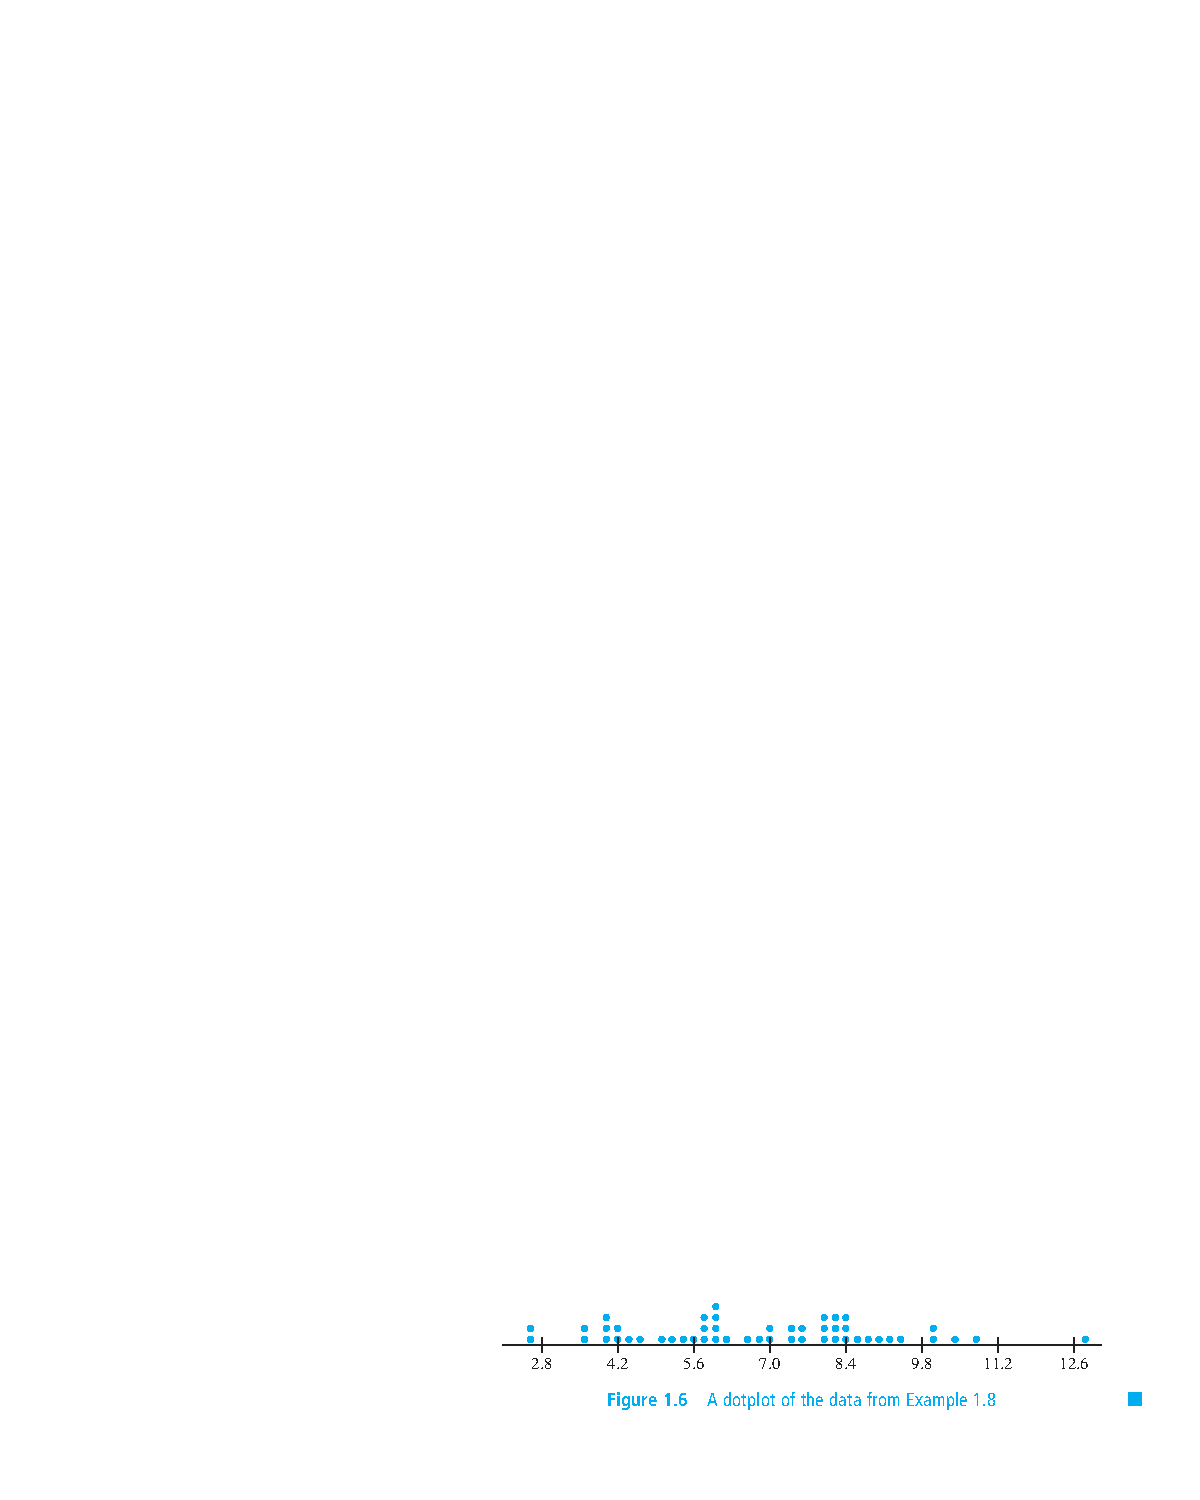
\includegraphics{figures/barplot.pdf}
\caption{A dotplot of the data from Example 1.8}
\label{fig:1}
\end{figure}


\subsection{Histogram}
\begin{defn}
A variable is \textbf{discrete} if its set of possible values either is finite or countable.
A variable is \textbf{continuous} if its set of possible values consists of an entire interval on the real line.
\end{defn}

\subsubsection{Discrete cases}
Frequency $ = $ number of times a value occur in the dataset.

Relative Frequency $ = \frac{\text{number of times the value occurs}}{\text{number of observation in the dataset}}$

\vspace{4mm}

\textbf{Procedure}
\begin{enumerate}
  \item calculate the Frequency and Relative Frequency
  \item mark each value on a horizontal scale
  \item above each value, draw a rectangular whose height is the frequency or relative frequency of the value.
\end{enumerate}

\begin{figure}[H]
\centering
\begin{tikzpicture}
\begin{axis}[name =one,
width=2.5 in,
height=1.5in,
axis x line=center,
symbolic x coords={Male,Female},
xtick=data,
title= (a) frequency,
enlargelimits=true,
ymin=0, ymax=50,
]
\addplot[ybar,fill=red] coordinates {
	(Male,   24)
	(Female, 36)
	};
%amd
\end{axis}

\begin{axis}[name=two,at=(one.right of south east), anchor=left of south west,
width=2.5in,
height=1.5in,
axis x line=center,
symbolic x coords={Male,Female},
xtick=data,
title= (b) relative frequency,
enlargelimits=true,
ymin=0, ymax=1,
]
\addplot[ybar,fill=green] coordinates {
	(Male,   0.4)
	(Female, 0.6)
	};
%nvidia
\end{axis}
\end{tikzpicture}

\end{figure}

\subsubsection{Continuous cases}
Need to determine the size of each class.

\paragraph{(a) Equal class} similar to discrete case.

\begin{figure}[H]
\centering
\begin{tikzpicture}
\begin{axis}[
    ymin=0, ymax=50,
    minor y tick num = 3,
    area style,
    ]
\addplot+[ybar interval,mark=no] plot coordinates { (0,1 ) (20, 40) (40, 12) (60,15) (80, 26) (100, 0) };
\end{axis}
\end{tikzpicture}
\end{figure}

You can also use the relative frequency.

\paragraph{(b) The unequal class}
\begin{exmp}
  0-10K, 10K-20K, 20-30K, \dots, 500K-510K, 510K-520K, \dots 
  (a waste of space!) 
  
  $\Rightarrow $  0-10K, 10K-20K, 20K-30K, 30K-40K, 40K-50K,  50K-100K, 100K-200K
\end{exmp}

For the unequal class, frequency or relative frequency may mislead some people because of a wide range. Therefore, we use density.

\[ \text{Density} = \frac{\text{relative frequency of the class}}{\text{class width}}	\]

Use density as height to draw histogram within unequal class.
\subsubsection{Shape of histogram}
\begin{itemize}
  \item Mode: unimodal, bimodal, multimodal
  \item Symmetry: symmetric, positive skewed, negative skewed
\end{itemize}

\begin{figure}[H]
\centering
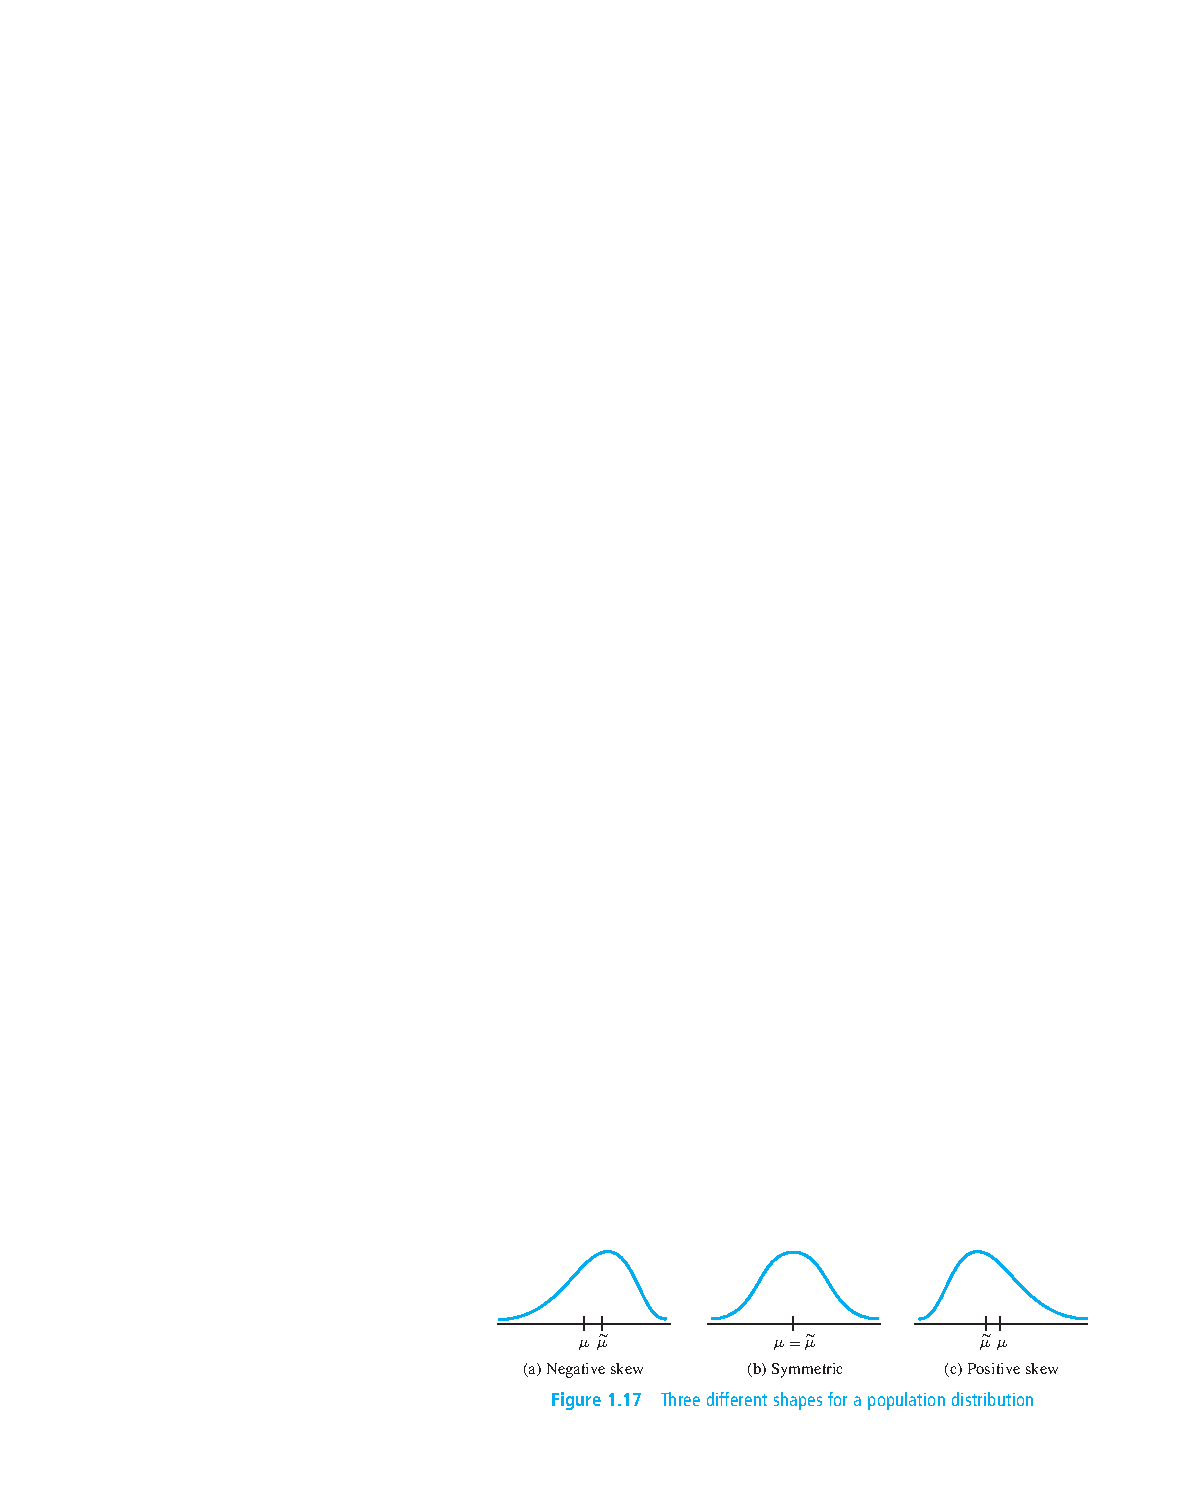
\includegraphics{figures/shape_histogram.pdf}
\caption{Three different shapes for a population distribution}
\label{fig:2}
\end{figure}

\section{Measures of Location and Variability}
\subsection{Location}

Observations: \[x_1,x_2 \dots x_n\]

Sample mean:
\[\bar{x}=\frac{\sum_{i=1}^{n} x_i}{n}\]

Sample median:
\[	\tilde{x}=\begin{cases}
\frac{n+1}{2}\text{th ordered value}, &\text{if } n \text{ is odd}\\
\frac{n}{2}\text{ or }\frac{n+2}{2}\text{th ordered value}. &\text{if }n\text{ is even}
\end{cases}	\]


\begin{itemize}
  \item symmetric: $x\approx \tilde{x}$
  \item positive skewed: $x>\tilde{x}$
  \item negative skewed: $x<\tilde{x}$
\end{itemize}

If you want your mean closer to your sample median. You can use \textbf{truncated mean}.

\subsection{Variability}
\begin{exmp}
Two dataset
  \begin{itemize}
    \item Dataset 1 \qquad 1,100 \qquad  $\bar{x}=50.5$ \qquad $\tilde{x}=50.5$
    \item Dataset 2 \qquad 50,51 \qquad  $\bar{x}=50.5$ \qquad $\tilde{x}=50.5$
  \end{itemize}
\end{exmp}

Sample Variance: \[S^2=\frac{\sum_{i=1}^{n} (x_i-\bar{x})^2}{n-1}\]

Sample Standard deviation (s.d): $S=\sqrt{S^2}$

Short-cut formula:
\[S^2=\frac{{\sum_{i=1}^{n} x_i^2} - n{\bar{x}}^2}{n-1}
\]
\begin{proof}
\[\sum_{i=1}^{n}(x_i-\bar{x})^2=
\sum_{i=i}^{n}(x_i^2+2x_i\bar{x}+{\bar{x}}^2)=
\sum_{i=i}^{n}x_i^2-2\bar{x}\sum_{i=1}^{n}x_i+
\sum_{i=i}^{n}\bar{x}^2 \]

Since 
\[\bar{x}=\frac{\sum_{i=1}^{n} x_i}{n}, \qquad n\bar{x}=\sum_{i=1}^{n} x_i \]

Substitute this, and the proof is done. 
\end{proof}

\begin{prop}
Let $x_1 \dots x_n$ be a sample, and $c$ be any nonzero constant.

\begin{enumerate}
\item Let $y_1=x_1+c,y_2=x_2+c,\dots,y_n=x_n+c$, then
\[\bar{y}=\bar{x}+c, S_y^2=S_x^2\]
\item Let $z_1=cx_1,z_2=cx_2,\dots,z_n=cx_n$, then
\[\bar{z}=c \bar{x}, S_z^2=c^2S_z^2\]
\end{enumerate}
\end{prop}

\subsection{Boxplot}
The simplest boxplot is based on the following five-number summary:

smallest $x_i$, \quad lower fourth,\quad median, \quad upper fourth, \quad largest $x_i$

\begin{defn}
Any observation farther than 1.5$f_s$ from the closest fourth is an \textbf{outlier}. An outlier is \textbf{extreme} if it is more than 3$f_s$ from the nearest fourth, and it is \textbf{mild} otherwise.
\end{defn}

Each mild outlier is represented by a closed circle and each extreme outlier by an open circle.

\begin{figure}[H]
\centering
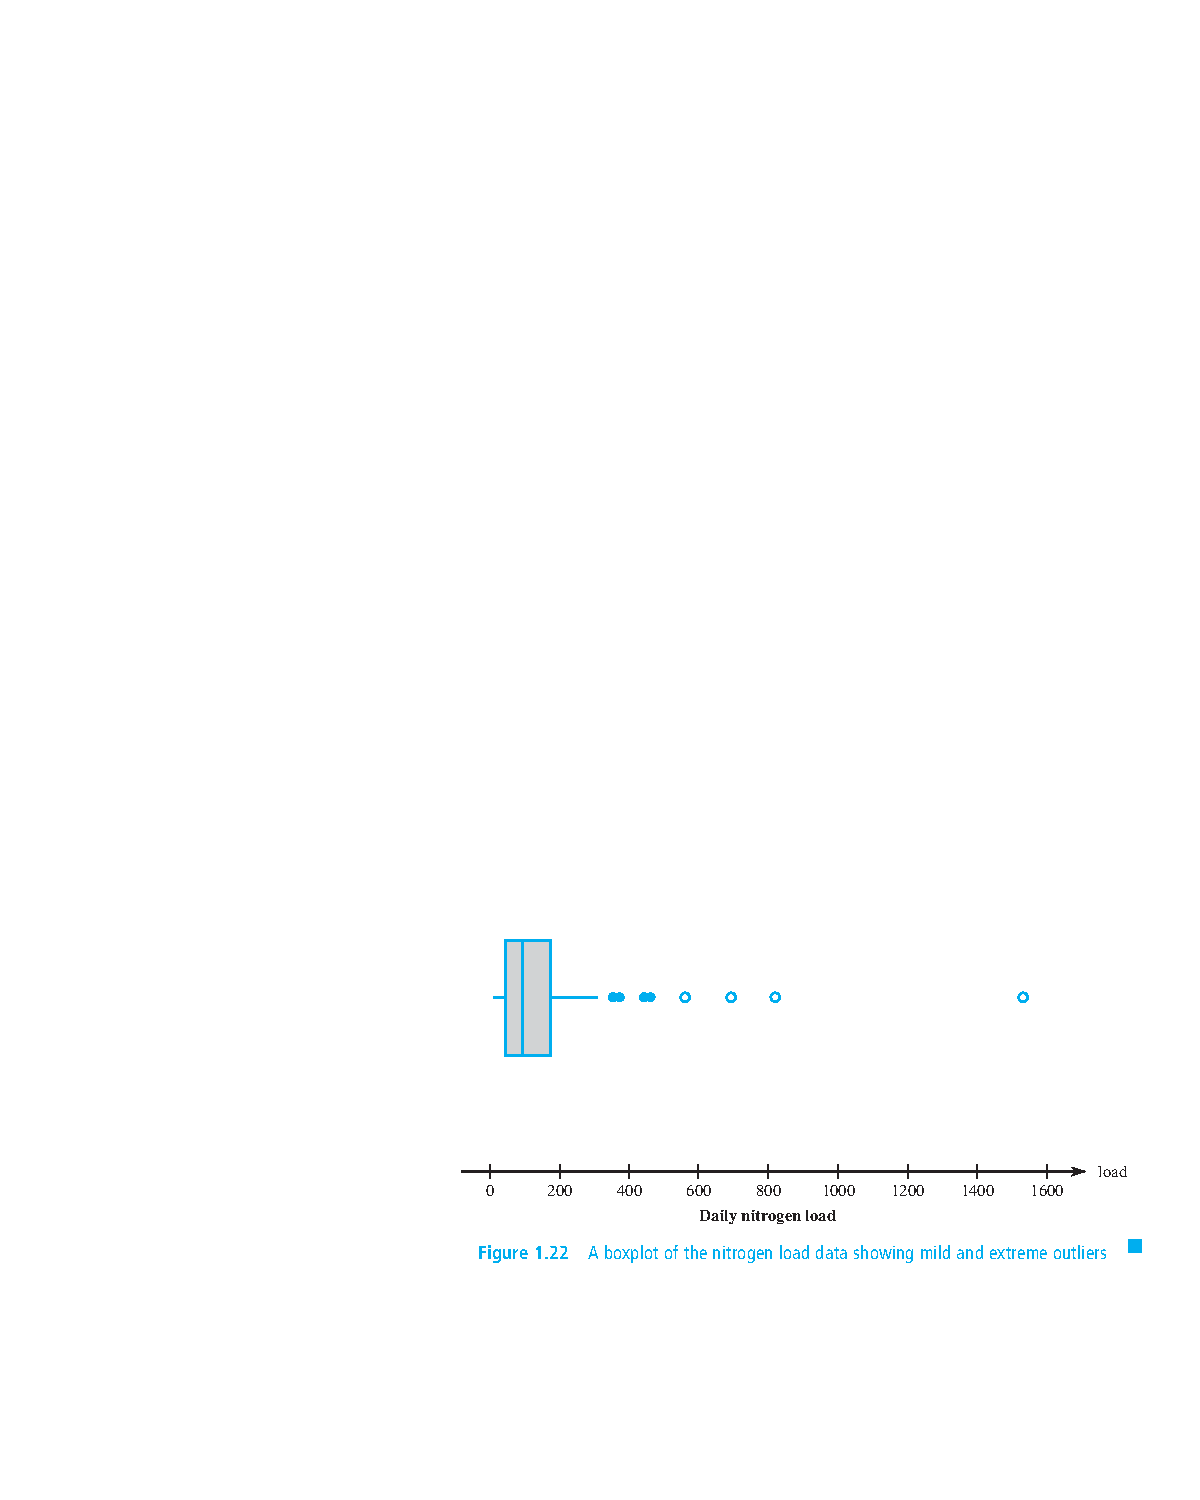
\includegraphics{figures/boxplot.pdf}
\caption{Boxplots That Show Outliers}
\label{fig:3}
\end{figure}

% chapter 2
% Last edit: 2017-5-4
\chapter{Probability}
\section{Sample Spaces and Events}

\begin{defn}
  An \textbf{experiment} is any action or process that generates observation.
\end{defn}

\begin{exmp}
  Flip a coin once, observe either H or T.
\end{exmp}

\begin{exmp}
  Roll a dice, observe one one spot, two spot \dots six spot.
\end{exmp}

\begin{exmp}
  Choose a card from a well-shuttled deck, observe a deck of cards.\footnote{Four suits: $\spadesuit$spade; $\heartsuit$heart; $\diamondsuit$diamond; $\clubsuit$club. 13 cards in each suit: A,2,3,\dots,10,J,\\Q,K.}
\end{exmp}

\subsection{The Sample Space of an Experiment}
\begin{defn}
  \textbf{Sample space} of an experiment, denoted by $\mathcal{S}$, is the set of all possible outcomes of the experiment.
\end{defn}

\begin{exmp}
  $\mathcal{S}=\{\text{H},\text{T}\}$
\end{exmp}

\begin{exmp}
  $\mathcal{S}=\{1,2,3,4,5,6\}$
\end{exmp}

\begin{exmp}
  $\mathcal{S}=\{A\spadesuit,2\spadesuit ,\dots, K\heartsuit\}$
\end{exmp}

\begin{exmp}
  Flip a coin twice, $\mathcal{S}=\{\text{HH},\text{HT},\text{TH},\text{HH}\}$
\end{exmp}

\subsection{Events}
\begin{defn}
  An \textbf{event} is a collection of outcomes of the sample space, denoted by $E$.
\end{defn}

\begin{exmp}
  $E=\{H\}$
\end{exmp}

\begin{exmp}
  $E=\{4,5,6\}$
\end{exmp}

\begin{exmp}
  $E=\{A\clubsuit,2\clubsuit,\dots,K\clubsuit\}$
\end{exmp}

\begin{exmp}
  $\mathcal{E}=\{HH,TT\}$
\end{exmp}

\subsection{Some Relations from Set Theory}
\begin{defn}
  The \textbf{union} of two events $A$ and $B$ is the event consisting of all outcomes that are either in $A$ or in $B$. Notation:$A\cup B$
\end{defn}

\begin{defn}
  The \textbf{intersection} of two events $A$ and $B$ is the event consisting of all outcomes that are in \textbf{both} $A$ or in $B$. Notation: $A \cap B$
\end{defn}

\begin{defn}
  The \textbf{complement} of an event  $A$ is the event consisting of all outcome in $\mathcal{S}$ but not in $A$. Notation: $A'$
\end{defn}


\begin{exmp}
  Roll a dice, $\mathcal{S}=\{1,2,3,4,5,6 \}$\\
  Let $A=\{1,2,3\}$, $B=\{1,3,5\}$\\
  $A\cup B=\{1,2,3,5\}$, $A \cap B=\{1,3\}$\\
  $A'=\{4,5,6\}$ , $B'=\{2,4,6\}$
\end{exmp}

\begin{defn}
  If $A$ and $B$ have no outcome in common, then they are \textbf{mutually exclusive} or \textbf{disjoint} $\Rightarrow$ $A\cap B=\varnothing$
\end{defn}

\begin{prop}
$A$ and $A'$ are disjoint.
\end{prop}


\begin{figure}[H]
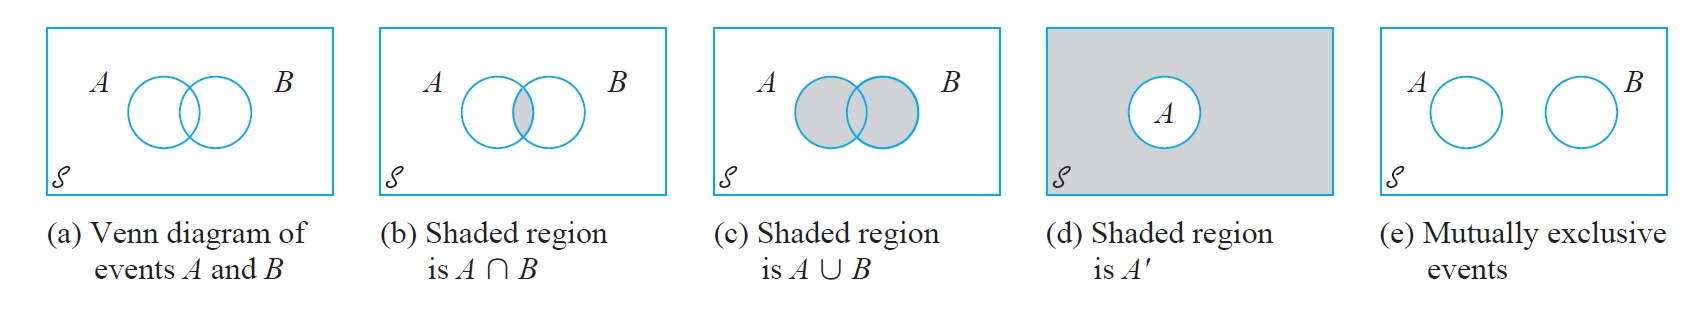
\includegraphics[width=15cm]{figures/venn_diagram.jpg}
\caption{Venn diagrams}
\label{fig:4}
\end{figure}

\begin{exmp}
  $(A\cup B)\cap C=(A \cap C)\cup(B \cap C)$
\end{exmp}


\section{Axioms, interpretations, and Properties of Probability}
Probability: Given a sample space $\mathcal{S}$, for any event $A\in \mathcal{S}$, assign a number, say $P(A)$, to it.
\begin{axio}
  For every event $A$, $P(A)\geq 0$.
\end{axio}

\begin{axio}
  $P(\mathcal{S})=1$
\end{axio}

\begin{axio}
If $A_1, A_2,A_3,\dots$is an infinite collection of disjoint events, then 
\[  P(A_1 \cup A_2\cup A_3 \cup \dots)=\sum_{i=1}^{\infty}P(A_i)	\]
\end{axio}

\begin{prop}
$P(\varnothing)=0$
\begin{proof}
Let $E_1=\varnothing,E_2=\varnothing,\dots E_n=\varnothing$
\[P(\varnothing \cup \varnothing \cup \dots \varnothing)=\sum_{i=1}^n P(\varnothing)\]
\[P(\varnothing)=nP(\varnothing)\]
\[P(\varnothing)=0\]
\end{proof}
\end{prop}

\begin{prop}
If $A$ and $B$ are disjoint, $P(A \cup B)=P(A)+P(B)$.
\begin{proof}
Let $E_1=A,E_2=B,E_3=\varnothing \dots E_n=\varnothing$. Then, we can prove it by Axiom 3.
\end{proof}
\end{prop}

\begin{exmp}
Flip a coin, $\mathcal{S}=\{H,T\}$
\[P(H)=0.89 \qquad P(T)=0.1\]
\[P(\mathcal{S})=P(H \cup T)=P(H)+P(T)=\boxed{0.99} \neq 1		\]

not a probability.
\end{exmp}

\begin{exmp}
Batteries come off an assembly line are tested one by one. The test will stop until a battery fails.
\[F:\text{faliure} \qquad S=\text{success}\]

Suppose $P(S)=0.99 \qquad P(F)=0.01$
\[\mathcal{S}=\{ F,SF,SSF,SSSF,\dots		\}\]
\[E_1=\{F\},E_2=\{SF\},E_3=\{SSF\},\dots		\]
\[P(\mathcal{S})=P(E_1 \cup E_2 \cup E_3 \dots)=P(E_1)+P(E_2)+P(E_3)+\dots\]
\[P(E_1)=0.01 \qquad P(E_2)=0.01\times0.99 \qquad P(E_3)=0.01\times 0.99^2\]
\[P(\mathcal{S})=0.01+0.99\times0.01+\dots=0.01\times\frac{1}{1-0.99}=1\]
\end{exmp}

\subsection{Interpreting Probability}
\begin{exmp}
If I flip a coin $10$ times, ref freq of H = \# of H /$10$. If I flip a coin $n$ times, ref freq of H = \# of H /$n$.

The probability of flipping a coin resulted in H= relative freq of H when $n\to \infty$. 
\[P(H)=\lim _{x \to \infty} \frac{\# of H}{n}\]
\end{exmp}

\subsection{How to calculate Properties of Probability}

\begin{prop}
$P(A')=1 -P(A) $
\begin{proof}
\[1=P(\mathcal{S})=P(A \cup A')=P(A)+P(A')\]
\end{proof}
\end{prop}
  
\begin{exmp}
Components connected in a series, each component has 0.3 probability of fail, and they fail independently.
   
\[A=\{\text{the system fails}\}\]
\[P(A)=P(\{ FSSSS,SFSSS,\dots\})\]
\[P(A)=1-P(\{\text{the system works}\})=1-P(SSSSS)=1-0.7^5\]
\end{exmp}
  
\begin{prop}
  If $A\cap B =\varnothing, P(A \cap B)=0 $
\end{prop}
  
\begin{prop}
 $ P(A \cup B)= P(A) +P(B) -P(A \cap B) $
\begin{proof}
Let $E = B \cap A' $, A and E are disjoint
  \[A \cup B = A \cup E\]
  \[P(A\cup B)=P(A \cup E)=P(A)+P(E)  \qquad (*)\]

Let $F= B\cap A$
  \[E \cup F =B \qquad E \cap F =\varnothing\]
  \[ P(B) = P(E \cup F)=P(E) + P(F)=P(E)+P(A\cap B)  \]
  \[P(E)= P(B)- P(A \cap B) \]

Plug in (*),\[  P(A \cup B)= P(A) +P(B) -P(A \cap B)  \]
\end{proof}
\end{prop}


\begin{exmp}
A card is drawn form a well-shuttled deck, what is the probability that it is a queen or a heart?
\begin{align*}
&Q=\{\text{the card is a Queen}\}\\
&H=\{\text{the card is a heart}\}
\end{align*}
\[P(Q \cup H)=P(Q)+P(H)-P(Q \cap H)=\frac{16}{52}\]
\end{exmp}

\begin{exmp}
In pccw, 80\% of the customers subscribed to cable TV. 30\% of the customers subscribed to Internet. 25\% of the customers subscribed to both.
Randomly select one customer, what is the chance that the person has either TV or Internet.
\[C=\{\text{the customers subscribed to cable TV}\}\]
\[I=\{\text{the customers subscribed to Internet} \}\]
\[P(C)=0.8 \qquad P(I)=0.3 \qquad P(C\cap I)=0.25\]
\[P(C\cup I)=P(C)+P(I)-P(C\cap I)=\boxed{0.85}\]
\end{exmp}

\begin{prop}
\[ P(A \cup B \cup C)=P(A)+P(B)+P(C)-P(A \cap B)-P(B \cap C)-P(C \cap A)+P(A \cap B \cap C) \]
\end{prop}

\begin{exmp}
C: Cable \qquad I: Internet \qquad T:Telephone.\footnote{Acutually a mistake $P(I\cap T)=0.4$}
\begin{align*}
&P(C)=0.8 \qquad P(I)=0.3 \qquad P(T)=0.5	\\
&P(C\cap I)=0.25 \qquad P(I\cap T)=0.4 \qquad P(C\cap T)=0.3\\
&P(C\cap I \cap T)=0.2
\end{align*}
\[P(C\cup I \cup T)=P(C)+P(I)+P(T)-P(C \cap I)-P(C \cap T)-P(I \cap T)+P(C \cap I \cap T)=\boxed{0.85}\]
\end{exmp}

\subsection{Determining Probabilities Systematically}
Any event $A$ is a union of simple events, i.e. with only one outcome. Then

\[P(A)=\sum_{E_i \in A}P(E_i)\]

and we just need to determine $P(E_i)$.

\begin{exmp}
Toss a dice, $\mathcal{S}=\{1,2,3,4,5,6\}$
\[P(\text{the spots}<4)\]
\[A=\{\text{the spot}< 4 \}=\{1,2,3\}\]
\[E_i=\{i\};\qquad i=1,2,3,4,5,6\]
\[A=E_1 \cup E_2 \cup E_3 \qquad  P(A)=P(E_1)+P(E_2)+P(E_3)\]

Suppose 
\[P(1)=P(2)=P(6)=\frac{1}{9}\]
\[P(3)=P(4)=P(5)=\frac{2}{9}\]
\[P(A)=P(1)+P(2)+P(3)=\frac{4}{9}\]
\end{exmp}

\subsection{Equally Likely Outcomes}
Suppose $\mathcal{S}$ has $N$ outcomes, $E_1,\dots E_N$, they are equally likely to occur, then
\[P(E_i)=\frac{1}{N} \qquad i=1,2,\dots\]

Then 
\[P(A)=\frac{\text{\# of outcome in A}}{N}\]

\begin{exmp}
Toss a pair of fair dices. What is the chance that the sum of spots is 3?
\[N=36 \qquad \mathcal{S}=\{(1,1),(1,2),\dots ,(6,6)\}\]
\[A=\{\text{the sum of spots is 3}\}=\{(1,2),(2,1)\}\]
\[P(A)=\frac{2}{36}\]
\end{exmp}

\begin{exmp}
What is the chance that the sum of spots $\leq 4$?
\[B=\{\text{the sum of spots}\leq 4\}=\{(1,1),(1,2),(1,3),(2,1),(2,2),(3,1)\}\]
\[P(B)=\frac{6}{36}\]
\end{exmp}

\section{Counting Techniques}
\begin{exmp}
A new guy comes to HK. If there are 3 brands of cell phone, 4 telephone companies offer mobile service.

\end{exmp}

\subsection{Product Rule}
Select two elements in a row. The first element has $n_1$ choices, the second has $n_2$ choices. Then the number of pairs $ = n_1 \cdot n_2$.

In general: suppose a set consists of $K$ ordered elements (K-tuples), 1st element has $n_1$ choices, 2nd element has $n_2$ choices, 3rd element has $n_3$ choices,\dots. Then the number of different K-tuples is $n_1 n_2 \dots n_k$.


\subsection{Permutations and Combinations}
\begin{exmp}
70 students in the room choose 4 students to form a committee (secretary, treasury, officer 1, officer 2).
\begin{enumerate}
\item How many possible committees with position assigned?
\[70 \times 69 \times 68 \times 67=\frac{70!}{66!} \]
\item How many possible committees without position assigned?
\[{70 \choose 4} =\frac{70!}{4!66!}\]
\end{enumerate}
\end{exmp}

\begin{defn}
The number of \textbf{permutation} of size $k$n of $n$ objects is denoted as $P_{k,n}=\frac{n!}{(n-k)!}$.

In specific, $P_{n,n}=n!\qquad (0!=1)$
\end{defn}

\begin{defn}
Given $n$ distinct objects,any disordered subject of size $k$ is called a \textbf{combination} of size $k$. The number of combination of size $k$ of $n$ objects, is denoted as $C_{k,n}$ or $\binom nk=\frac{n!}{k!(n-k)!}$.
\end{defn}


\begin{exmp}
\[\{A,B,C,D,E\}\]
\begin{enumerate}
\item  Choose 3 letters, how many choices?
\[\binom 53 =10\]
\item  Choose 3 letters to form a word, how many different words?
\[P_{3,5}=60\]
\end{enumerate}
\end{exmp}

\begin{prop}
\[k!\times C_{k,n}=\binom nk \times k!=P_{k,n}\]
\end{prop}

\begin{exmp}
"Birthday Paradox" 

365 different dates, $n$ students.
\begin{align*}
&P\{\text{at least two students share the same birthday}\}\\
&=1-P\{\text{every one has a diffrent birthday}\}\\
&=1-\frac{P_{n,365}}{365^n}
\end{align*}

If $n=50$, $P=97\%$

If $n=100$, $P=99.99997\%$
\end{exmp}


\section{Conditional Probability}
\begin{exmp}
52 cards. One card is dealt, and the another card is dealt.
\begin{enumerate}
\item P(the second card is 7 of clubs)
$=\frac{1}{52}$
\item P(the second card is 7 of clubs given the first is J of spade)
$=\frac{1}{51}$
\item P(the first card is J of spade, and the second card is 7 of clubs)
$=\frac{1}{P_{2,52}}=\frac{1}{52\times 51}$
\item P(the first card is J of spade)
$=\frac{1}{52}$
\end{enumerate}

So P(B given A)=$\frac{P(A \cap B)}{P(A)}$
\end{exmp}

\begin{exmp}
Fishing in the sea
\begin{center}
\begin{tabular}{c|c|c}
\hline
 & Walleye & Pike\\
 \hline
 Sam & 2 &3\\
 \hline
 I & 1 &5\\
 \hline
\end{tabular}
\end{center}

Randomly pick one, found, it is s Walleye. What is the chance that it is caught by me?
\begin{align*}
&A=\{\text{Walleye}\}\\
&B=\{\text{Caught by me}\}\\
&P(A)=\frac{3}{11} \qquad P(B)=\frac{6}{11}\\
&P(B\text{ given }A)=\frac{P(A \cap B)}{P(A)}=\boxed{\frac{1}{3}}
\end{align*}
\end{exmp}

\subsection{The Definition of Conditional Probability}
\begin{defn}
For any two events $A$ and $B$, with $P(B)>0$, the conditional probability of $A$ given that $B$ has occurred is defined by
\[P(A|B)=\frac{P(A \cap B)}{P(B)}\]
\end{defn} 

\begin{exmp}
Of all costumers purchasing computers, 60\% of them include M\$ Word; 50\% of them include M\$ Excel; 30\% of them include both.
\begin{align*}
&A=\{\text{Word is included}\} 	\\
&B=\{\text{Excel is included}\}	
\end{align*}
\[P(A|B)=0.6 \qquad P(B|A)=0.5\] 
\[P(A|B)\neq P(B|A)\]
\end{exmp}

\textbf{Recall}:
Axioms of probability

\begin{enumerate}
\item  For every event $A$, $P(A)\geq 0$.
\item  $P(\mathcal{S})=1$
\item
If $A_1, A_2,A_3,\dots$is an infinite collection of disjoint events, then 
\[  P(A_1 \cup A_2\cup A_3 \cup \dots\cup A_n)=\sum_{i=1}^{n}P(A_i)	\]
\end{enumerate}

Similarly,
\begin{enumerate}
\item  For every event $A$, $P(A|B)\geq 0$.
\item  $P(B|B)=1$
\item  If $A_1, A_2,A_3,\dots$is an infinite collection of disjoint events, then 
\[  P(A_1 \cup A_2\cup A_3 \cup \dots\cup A_n|B)=\sum_{i=1}^{n}P(A_i|B) \]
\end{enumerate}

\begin{exmp}
A new magazine publishes 3 columns.

"Art"(A),"Boobs"(B),"Cinema"(C).
Research shows the reading habits

\begin{center}
\begin{tabular}{ccccccc}
\hline
$A$ & $B$ & $C$ & $A\cap B$ & $A\cap C$ & $B\cap C$ & $A \cap B\cap C$\\
\hline
0.14&0.23&0.37&0.08&0.09&0.13&0.05\\
\hline
\end{tabular}
\end{center}

Randomly select one reader

(1)
\[P(A|B)=\frac{P(A \cap B)}{P(B)}=\boxed{\frac{8}{23}}\]

(2)
\begin{align*}
P(A|B\cup C)&=\frac{P(A\cap (B\cup C) )}{P(B\cup C)}\\
&=\frac{P\big( (A\cap B)\cup(A \cap C) \big)}{P(B)+P(C)-P(B \cap C)}\\
&=\frac{P(A\cap B)+P(A\cap C)-P(A\cap B\cap C)}{P(B)+P(C)-P(B \cap C)}
\end{align*}

(3)

$P(A|A \cup B \cup C)$: What is the probability that the reader read "Art" Column given that  he/she reads at least one column?
\begin{align*}
P(A|A \cup B \cup C)&=\frac{P(A \cap (A \cup B \cup C) )}{P(A \cup B \cup C)}=\frac{P(A)}{P(A \cup B \cup C)}\\
&=\frac{P(A)}{P(A)+P(B)+P(C)-P(A \cap B)-P(B \cap C)-P(C \cap A)+P(A \cap B \cap C)}\\
&=\boxed{\frac{14}{49}}
\end{align*}

(4)
\begin{align*}
P(A \cup B |C)=&\frac{P((A \cup B)\cap C)}{P(C)}\\
=&\frac{P(A \cap C) +P(B \cap C)-P(A \cap B \cap C)}{P(C)}=\boxed{\frac{17}{37}}
\end{align*}
\end{exmp}

\subsection{The Multiplication Rule for $P(A\cap B)$}
\begin{prop}
\[P(A \cap B)=P(A)P(B|A)=P(B)P(A|B)\]
\end{prop}

\begin{exmp}
Two cards are dealt.

\[P(\text{1st is J of spade and 2nd is 7 of heart})=P(A)P(B|A)=\frac{1}{52} \times \frac{1}{51}\]
\end{exmp}

\begin{exmp}
Same scenario

\[ A=\{\text{1st is a club}\} \]
\[ B=\{\text{2nd is a club}\}\]
\[P(A\cap B)=P(A)P(B|A)=\frac{13}{52} \times \frac{12}{51}\]
\[C=\{\text{3rd card is a heart}\} \]
\[P(A \cap B\cap C)=P(A\cap B)P(C|A \cap B)=P(A)P(B|A)P(C|A \cap B)=\frac{13}{52} \times \frac{12}{51} \times \frac{13}{50}\]
\end{exmp}

\begin{prop}
\[P(A_1 \cap A_2 \dots \cap A_k)=P(A_1)P(A_2|A_1)P(A_3|A_1\cap A_2)\dots P(A_k|A_1\cap A_2\dots\cap A_{k-1})\]
\end{prop}

\begin{exmp}
Same scenario
\begin{align*}
& A=\{\text{1st is a club}\} \\
& B=\{\text{2nd is A of club}\} \\
& C=\{\text{3rd is 2 of club}\} \\
\end{align*}
\[ P(A \cap B\cap C)=P(C)P(B|C)P(A|B\cap C)=\frac{1}{52}\times\frac{1}{51}\times\frac{11}{50} \]

Introduce $D=\{\text{1st is either 3,4,\dots K of club}\}$
\[P(A \cap B\cap C)=P(D\cap B\cap C)=\frac{11}{52}\times\frac{1}{51}\times\frac{1}{50}\]
\end{exmp}

\subsection{Bayes' Theorem}
\begin{theo}
  The Law of Total Probability

  Let $A_1, . . . , A_k$ be mutually exclusive and exhaustive events. Then for any other event $B$,
  \[ P(B)=\sum_{i=1}^{k} P(B|A_i)P(A_i)\]
\end{theo}

\begin{exmp}
A store sells 3 brands of game consoles

\begin{center}
 \begin{tabular}{l|ccc}
 \hline
 Brand & 1 & 2 & 3 \\
 \hline
 Proportion & 50\% & 30\% & 20\%\\
 \hline
 \end{tabular}  
\end{center}

A one year warranty is offered, known 

\begin{center}
    \begin{tabular}{l|ccc}
    \hline
    Brand & 1 & 2 & 3 \\
    \hline
    Under warranty & 25\% & 20\% & 10\%\\
    \hline
  \end{tabular}
\end{center}
  \[A_i=\{\text{bought brand }i\} \qquad i=1,2,3\]
  \[B=\{\text{needs repaire under warranty}\} \]
  \[P(A_1)=0.5 \qquad P(A_2)=0.3 \qquad P(A_3)=0.2\]
  \[P(B|A_1)=0.25 \qquad P(B|A_2)=0.2 \qquad P(B|A_3)=0.1\]
  
  Q1:\[P(B'|A_1)=1-P(B|A_1)=0.75\]

  Q2:\[P(B)=P(A_1)P(B|A_1)+P(A_2)P(B|A_2)+P(A_3)P(B|A_3)=0.205\]

  Q3:\begin{align*}
  &P(A_1|B)=\frac{P(A_1 \cap B)}{P(B)}=\frac{P(A_1)P(B|A_1)}{P(B)}=0.61\\
  &P(A_2|B)=0.29 \\
  &P(A_3|B)=0.10\\
  \end{align*}
\end{exmp}

\begin{theo}
  Bayes' Theorem
  \[P(A_i|B)=\frac{P(A_i \cap B)}{P(B)}=\frac{P(A_i)P(B|A_i)}{\sum_{i=1}^k P(A_k)P(B|A_i)}    \]
\end{theo}

\begin{exmp}
$\frac{1}{1000}$ adults has a rare disease.

99\% of people with the disease can be found positive

20\% of people without the disease can be found positive

Randomly select a person and test him. Suppose the result is positive. What is the chance that he really has the disease? 

Let
\[	A=\{\text{the individual has the disease} \}		\]
\[	A'=\{\text{the individual does not have the disease} \}		\]
\[	B=\{\text{that positive} \}		\]
\[	P(A)=\frac{1}{1000} \qquad P(B|A)=0.99 \qquad P(B|A')=0.20	\]

Question:
\[	P(A|B)=\frac{P(A \cap B)}{P(B)}=\frac{P(A)P(B|A)}{P(A)P(B|A)+P(A')P(B|A')}		\]

Because $A$ and $A'$ are portions of $\mathcal{S}$
\[	=\frac{0.001\times 0.99}{0.001\times 0.99+ 0.999\times 0.2}=0.493\%		\]
\end{exmp}
\section{Independence}
\begin{defn}
Two events A and B. If A and B are \textbf{independent}, then
\[P(A\cap B)=P(A)P(B) \]

Note that $P(A \cap B)=P(A)P(B|A)$ apply for any condition.
\[  P(B)=P(B|A) \]

event $A$ has nothing to do with event B.
\end{defn}

\begin{exmp}
  Roll a dice once. $P(i)=\frac{1}{6}; i=1,2,\dots,6$
  \[  A=\{2,4,6\},   B=\{1,2,3\},   C=\{1,2,3,4\} \]
  \[  P(A)=\frac{3}{6}=\frac{1}{2} \]
  \[ P(A|B)=\frac{P(A\cap B)}{P(B)}=\frac{1/6}{3/6}=\frac{1}{3} \]
  \[ P(A|C)=\frac{P(A\cap C)}{P(C)}=\frac{2/6}{4/6}=\frac{1}{2} \]

So $A$ and $C$ are independent. $A \not\!\perp\!\!\!\perp B$
\end{exmp}

\begin{prop}
if $A$ and $B$ are independent
\begin{itemize}
  \item $A'$ and $B'$ are independent
  \item $A'$ and $B$ are independent
  \item $A$ and $B'$ are independent
\end{itemize}
\end{prop}

\begin{exmp}
  Toss a fair coin repeatedly until the first H occurs.
  \[A=\{\text{at least 5 tosses result in the first H}\}\]
  \[P(A)= \quad ?\]
	 
Assume the tossing are independent.
\[A=\{TTTTH\}\cup	\{TTTTTH\} \cup \dots	\]
\begin{align*}
P(A)&=P(\{TTTTH\})+\dots =(P(T))^4 P(H)+(P(T))^5 P(H)\\
&=\left(\frac{1}{2}\right)^5+\left(\frac{1}{2}\right)^6+\dots=\frac{1}{16}
\end{align*}
\end{exmp}

\subsection{Independence of More Than Two Events}
\begin{defn}
$A_1,A_2,\dots A_k$ are events. If for any indices $i,\dots, i_k$
\[P(A_1 \cap A_2 \cap \dots A_k)=P(A_1)P(A_2)\dots P(A_k)\]

Then $A_1,A_2,\dots A_k$ are said to be mutually independent.
\end{defn}

\begin{exmp}
Component works with probability 0.9, and they work independently.
\[P(\text{system works})\]

Let
\begin{align*}
&A_i=\{ \text{the }i\text{th component works} \}	\\
&P(A_i)=0.9	\\
&P(\text{system works})=P\left( (A_1 \cap A_2)\cup(A_3 \cap A_4) \right)=0.9639\\
\end{align*}
\end{exmp}

\section{Challenge Question 1}
Monty Hall problem.

\url{https://en.wikipedia.org/wiki/Monty_Hall_problem}


\section{Problem in Previous Mid-term Test}
 \begin{exmp}
 \begin{align*}
   &D=\{\text{David makes a right decision}\}	\\
   &J=\{\text{John makes a right decision}\}	\\
   &P=\{\text{Peter makes a right decision}\}	
 \end{align*}

David and Peter make decision independently.
  \[  P(D) = 0.7 \qquad P(D|J)=0.9 \qquad P(D'|J')=0.8  \]
  \[  P(J|P)=0.3 \qquad P(J'|P')=0.2 \qquad P(D \cap J\cap P)=0.1 \]

  Question: 
  
  (1) $P(J)= \quad ?$ 
  
  (2) $P(P)= \quad ?$ 
  
  (3) $P(\text{at least two make right decision})=\quad ?$
\end{exmp}

\begin{solution}
  (1)
  \begin{align*}
  &0.9=P(D|J)=\frac{P(D \cap J)}{P(J)}  \\
  &0.8=P(D'|J')=\frac{P(D'\cap J')}{P(J')}=\frac{P(D\cup J)'}{1-P(J)}=\frac{1-P(D\cup J)}{1-P(J)}
  \end{align*}
  \[P(D\cup J)=P(D)+P(J)-P(D \cap J)=0.7+P(J)-P(D \cap J)\]
  \[P(J)=\frac{5}{7}\]

  (2) Similar to (1)

  (3)
  \[P(\text{at least two make right decision})\]
  
Method A:
\begin{align*}
  &=1-P(\text{no more than 1 make right decisions})\\
  &=1-P(D \cap J \cap P')-P(D' \cap J \cap P')-P(D' \cap J' \cap P)-P(D' \cap J' \cap P')
\end{align*}

Method B:
\[ =P(A \cap B)+P(B \cap C) + P(C \cap A)-2 P(A\cap B \cap C)\]
\end{solution}
% chapter 3
% Last edit: 2017-4-28
\chapter{Discrete Random Variables}
\section{Random Variable}
\begin{defn}
  For a given sample space $\mathcal{S}$ of some experiment, a random variable (rv) is any rule that associates a number with each outcome in $\mathcal{S}$. In mathematical language, a random variable is a function whose domain is the sample space
and whose range is the set of real numbers.
\end{defn}

\begin{exmp}
Flip a coin, $\mathcal{S}=\{\text{H} ,\text{T} \}$
\[X(H) = 1 \qquad X(T) =0 \]
\end{exmp}

\begin{exmp}
Randomly pick a student, height
\[X(\text{height}\geq \text{6 feet})=1  \qquad X(\text{height}\leq \text{6 feet})=0
\]
\end{exmp}

\begin{defn}
Any r.v. whose possible values are 0 and 1 is called a \textbf{Bernoulli random variable}.
\end{defn}

\begin{exmp}
Randomly pick a student, phone brand
\[X(\text{Apple})=1 \qquad  X(\text{Samsung})=0	\]
\end{exmp}

\begin{exmp}
Waiting MTR at Kowloon Tong
\[X(\text{waiting time})=\text{waiting time}\]
\end{exmp}

\subsection{Two Types of Random Variables}
\begin{defn}
a \textbf{discrete} r.v. whose possible values are either finite or countable.

a \textbf{continuous} r.v. is a r.v. whose possible values consist of an entire interval on the real lines.
\end{defn}

\section{Probability Distributions for Discrete Random Variables}

\begin{defn}

$\mathcal{S}$ is a sample space, $X(s)$ is a r.v. $p(x)=P(s\in \mathcal{S};X(s)= x) $ is called the probability mass function (p.m.f) or probability distribution function (p.d.f) of $x$.
\end{defn}

\begin{exmp}
\[	\mathcal{S}=(5 \text{ feet}, 7 \text{ feet} )		\]
\[	X(s)=\begin{cases}
1, & \text{if} \quad s\geq 6 \text{ feet} \\
0. & \text{if} \quad s\leq 6 \text{ feet}
\end{cases}		\]
\[	P(X=1)=P(s \geq 6 \text{ feet})\]
\end{exmp}

\begin{exmp}
Six lots of components that the \# of defectives are listed as follows
\begin{center}
\begin{tabular}{c|cccccc}
\hline
lot				& 1 & 2 & 3 & 4 & 5 & 6 \\
\hline
\# of defectives& 0 & 2 & 0 & 1 & 2 & 0 \\
\hline
\end{tabular}
\end{center}

One of those is randomly selected. $X$ = \# of defectives in the selected lot
\[	P(X=0)=P(\{1,3,6\})=\frac{1}{2}		\]
\[	P(X=1)=P(\{4\})=\frac{1}{6}			\]
\[	P(X=2)=P(\{2,5\})=\frac{1}{3}		\]
\end{exmp}

\begin{exmp}
Five person 1,2,3,4,5 are blood donors. Among them, only 1 and 2 have "O" type. Collect their blood in a random segment, $X=\text{\# of typing neccessary to get the first "O" type}$.
\[	X = 1,2,3,4		\]
\[	P(X=1)=P(\text{typing after the first trail})=\frac{2}{5} \]
\end{exmp}

\subsubsection{Review}
X is a discrete r.v.
\begin{enumerate}
\item Support $x \in \mathcal{D}$
\item p.m.f $p(x)=P(s\in \mathcal{S};X(s)= x), \quad\forall x \in \mathcal{D}$
\end{enumerate}


\subsection{The Cumulative Distribution Function}
\begin{exmp}
Roll a dice. Let $x$= \# of spots. What is the probability that $x \leq 5$
\[	\mathcal{D}=\{1,2,3,4,5,6\}		\]
\[	P(1)=P(2)=\dots=P(6)=\frac{1}{6}		\]
\[	P(X \leq 5)=P(\{1,2,3,4,5\})=P(1)+P(2)+P(3)+P(4)+P(5)=\frac{5}{6}	\]
\[F(x)=\begin{cases}
P(X \leq x)=0 &\text{if } x < 1 \\
P(X \leq x)=\frac{1}{6} &\text{if } 1 \leq x < 2 \\
\dots \\
P(X \leq x)=1 &\text{if } x \geq 6 \\
\end{cases}\]
It is called step function.
\end{exmp}

\begin{defn}
The Cumulative Distribution Function (c.d.f) of a r.v $X$ is defined as 
\[	F(x)=P(X\leq x)=\sum_{y\leq x}p(y) \]
\end{defn}

\begin{exmp}
a r.v $Y$

\begin{center}
\begin{tabular}{c|cccc}
\hline
$y$  & 1 & 2 & 3 & 4\\
\hline
$p(y)$  & 0.4 & 0.3  & 0.2  & 0.1 \\
\hline
\end{tabular}
\end{center}


\[F(y)=P(Y\leq y)=\begin{cases}
0 &\text{if } y < 1 \\
0.4 &\text{if } 1 \leq y < 2 \\
0.7 &\text{if } 2 \leq y < 3 \\
0.9 &\text{if } 3 \leq y < 4 \\
1 &\text{if } y \geq 4 \\
\end{cases}
\]
\end{exmp}

\begin{exmp}
Toss a coin until the first head. Suppose $P(\text{Head})=p$, $P(\text{Tail})=q=1-p$, $x=\text{\# of toses until the first head}$
\[\mathcal{D}=\{1,2,3,\dots\}\]
\[p(x)=q^{x-1}p, \qquad x=1,2,3,\dots\]
\[F(x)=P(X \leq x)=\sum_{y \leq x}p(y)=\sum_{y \leq x}q^{y-1}p=p \frac{1-q^{\floor*{x}}}{1-q}=1-q^{\floor*{x}}\]
where $\floor*{x}$ is the largest integer $\leq x$ (floor function).
\[F(x)=\begin{cases}
0, & \text{if } x <0 \\
1-q^{\floor*{x}}. &\text{if } x\geq 0\\
\end{cases}\] 
\end{exmp}

\subsubsection{How do we get p.m.f from c.d.f}
In examples thus far, the cdf has been derived from the pmf. This process can be reversed to obtain the pmf from the cdf whenever the latter function is available.
\[P(X=3)=P(x\leq 3)-P(x \leq 2)=F(3)-F(2)\]
Suppose $X$ takes integer values, for any integers $a$ and $b$,
\[P(a\leq X \leq b)=P( X \leq b)-P(X \leq a-1)=F(b)-F(a-1)\]
Generally, for $a$ and $b$
\[P(a\leq X \leq b)=F(b)-F(a_-)\]
Here $a_-$ is the largest integer value that is strictly less than $a$. If $a=2$, $\floor*{a}=2$, $a_-=1$  

\section{Expected Values}
\begin{exmp}
"Russian roulette"

Bet even or odd. Bet \$1 on even, I will win \$1 if indeed it is even, and I will lose \$1 if it is odd, or 0, or 00.

Expected value
\[	\frac{18}{38}\times1+\frac{20}{38}\times(-1)=-\frac{2}{38}	\]

\end{exmp}

\subsection{The Expected Value of X}
\begin{defn}
Let X be a discrete rv with set of possible values $\mathcal{D}$ and pmf $p(x)$. The expected value or mean value of $X$, denoted by $E(X)$ or $\mu_X$ or just $\mu$, is
\[E(X)=\sum_{x\in \mathcal{D}} x p(x)\]
\[x=\begin{cases}
1,&\text{w.p.}\frac{18}{38} \\
-1,&\text{w.p.}\frac{20}{38}
\end{cases}\]
\[ E(X)=-\frac{2}{38}\]
\end{defn}

\begin{exmp}
X is a Bernoulli r.v
\[p(x)=\begin{cases}
p, & \text{if} \quad x=1\\
1-p. & \text{if} \quad x=0
\end{cases}\]
\[E(X)=1 p+0 (1-p)=p\]
\end{exmp}

\begin{exmp}
A newly-wed couple want a girl. Their plan is to keep having children until they get a girl.
\[  X=\text{\# of children when the girl is born}   \]
\[  P(\text{boy})=p \qquad P(\text{girl})=1-p=q     \]
\[	p(x)=p^{x-1}q \qquad x=1,2,3,\dots	\]
\[	E(X)=\sum_{x=1}^{\infty} xp^{x-1}q= q\sum_{x=1}^{\infty}xp^{x-1}	\]
\[	S=p^0+2p^1+3p^2+4p^3+\dots \]
\[	pS=p^1+2p^2+3p^3+4p^4+\dots \]
\[	(1-p)S=p^0+p^1+p^2+p^3+p^4+\dots=\frac{1}{1-p}\]
\[	E(X)=q\frac{1}{(1-p)^2}=\frac{1}{q}\]
Another method to calculate $\sum_{x=1}^{\infty} xp^{x-1}q$
\[	\sum_{x=1}^{\infty} xp^{x-1}=\sum_{x=1}^{\infty}(p^{x})'=\Big( \sum_{x=1}^{\infty}p^{x} \Big)'	\]
\end{exmp}

\begin{exmp}
\[	p(k)=\frac{1}{k^2}\frac{6}{\pi^2}	\qquad k=1,2,3,\dots\]
Verify \[\sum_{k=1}^{\infty} p(k)=1\]
\[E(x)=\sum_{k=1}^{\infty} k\frac{1}{k^2}\frac{6}{\pi^2}		=\frac{6}{\pi^2}\sum_{k=1}^{\infty}\frac{1}{k}=\infty	\]
\end{exmp}


\subsection{The Expected Value of a Function}
\begin{prop}
\[E(h(X))=\sum_{x\in \mathcal{D}}h(x)p(x)\]
\end{prop}

\begin{exmp}
\# of cylinders in the engine of the next car to be turned up.

Cost for $x$ cylinders
\[	h(x)=20+3x+0.5 x^2		\]
History shows that 
\begin{center}
  \begin{tabular}{c|ccc}
  \hline
  $x$  & 4 & 6 & 8 \\
  \hline
  $p(x)$  & 0.5 & 0.3  & 0.2  \\
  $h(x)$  & 40 & 56 & 76 \\
  \hline
  \end{tabular}
\end{center}

  
  \vspace{4mm}
 \[	E(h(x))=40\times0.5 +56\times 0.3+76\times 0.2 = \boxed{52}\]
\end{exmp}


\subsection{Rules of Expected Value}
\begin{prop}
Let $a$ and $b$ be two constant, $X$ r.v
\[E(aX+b)=aE(X)+b\]
Particularly,
\[\text{if} \quad b=0, \quad E(aX)=aE(X)\]
\[\text{if} \quad a=0, \quad E(X+b)=E(X)+b\]
\end{prop}

\begin{exmp}
  A computer store has purchased three computers of a certain type at \$500 apiece. It will sell them for \$1000 apiece. The manufacturer has agreed to repurchase any computers still unsold after a specified period at \$ 200 apiece. Let $X$ denote the number of computers sold.
\begin{center}
\begin{tabular}{c|cccc}
\hline
$x$ & 0 & 1 & 2 & 3 \\
\hline
$p(x)$  & 0.1 & 0.2  & 0.3  & 0.4 \\
\hline
\end{tabular}
\qquad $E(X)=2$
\end{center}

\[	Y=1000X+200(3-X)-1500=800X-900\]
\[	E(Y)=800E(X)-900=700\]
\end{exmp}

\subsection{The Variance of X}
\begin{exmp}
\qquad
\begin{tabular}{c|cccccc}
\hline
$x$ & 1 & 2 & 3 & 4 & 5 & 6 \\
\hline
$p(x)$  & $\frac{1}{6}$ & $\frac{1}{6}$  & $\frac{1}{6}$  & $\frac{1}{6}$ & $\frac{1}{6}$ & $\frac{1}{6}$\\
\hline
\end{tabular}

\[E(X)=\frac{7}{2}\]
  
\begin{center}
\begin{tabular}{c|cc}
\hline
$x$ &  3 & 4  \\
\hline
$p(x)$  & $\frac{1}{6}$ & $\frac{1}{6}$  \\
\hline
\end{tabular}
\end{center}

\[E(X)=\frac{7}{2}\]  
\end{exmp}

\begin{defn}
X is a discrete random variable $E(X)=\mu$, 
\[\sigma_{x}^2=Var(X)=E((X-\mu)^2)=\sum_{x \in \mathcal{D}} (x-\mu)^2p(x)\]
\[\sigma_x=s.d(X)=\sqrt{Var(X)}\]
\end{defn}

For Ex(1), $Var(X)=2.92$; For Ex(2), $Var(X)=0.25$.


\subsection{Shortcut Formula}
\begin{prop}
\[Var(X)=E(X^2)-(E(X))^2\]
\begin{proof}
\begin{align*}
Var(X)=& E((X-\mu)^2)= E(x^2-2X\mu+\mu^2)\\
=&E(X^2)+E(-2X\mu)+E(\mu^2) = E(X^2)-2\mu E(X)+\mu^2 \\
=& E(X^2)-2\mu \mu+\mu^2 = E(X^2)-(E(X))^2
\end{align*}
\end{proof}
\end{prop}

\subsection{Rules}
\begin{prop}
\[Var(aX+b)=a^2 Var(X)\]
\[s.d(aX+b)=|a| s.d(X)\]
since $a$ could be negative.
\end{prop}

\begin{exmp}
Computer store
\[Y=800X-900\]

\begin{center}
\begin{tabular}{c|cccc}
\hline
$x$ & 0 & 1 & 2 & 3 \\
\hline
$p(x)$  & 0.1 & 0.2  & 0.3  & 0.4 \\
\hline
\end{tabular}
\end{center}

\[Var(Y)=Var(800X-900)=800^2 Var(X)\]
\[E(X)=2 \qquad E(X^2)=5\]
\[Var(Y)=800^2(5-2^2)=640000\]
\end{exmp}


\section{The Binomial Probability Distribution}
Recall $X \sim Bernobli(p)$
\[p(0)=1-p \qquad p(1)=p\]

\begin{exmp}
Flip a coin 3 times independently. 
$X$=\# of Heads. What's the distribution of $X$?
\[\mathcal{D}=\{0,1,2,3\}\]
\begin{center}
\begin{tabular}{r|c|l}
\hline
       &  $x$  & $p(x)$ \\
    \hline
    TTT & 0 & $(1-p)^3$ \\
    HTT, THT, TTH  & 1 & $3p(1-p)^2$ \\
    HHT, HTH, THH  & 2 & $3p^2 (1-p)$ \\
    HHH & 3 & $p^3$ \\
\hline
\end{tabular}
\[\sum p(x)=1\] 
\end{center}
\end{exmp}

\subsection{The Binomial Random Variable and Distribution}
Generally, $n$ Bernouli trails, independently. the success rate of each trail is constant $p$, then the \# of success out of these $n$ trails is a \textbf{Binomial} r.v, denoted as $X \sim Bin(n,p)$

If $X \sim Bin(n,p)$,
\[P(X=x)=\binom nx p^x (1-p)^{n-x}  \qquad x=0,1,\dots n\]
Back to the Ex, \[P(X=0)=\binom 30 p^0 (1-p)^3=(1-p)^3\]

\subsection{The Mean and Variance of X}
\begin{prop}
If $X \sim Bin(n,p)$,
\[E(X)=np \qquad Var(X)=np(1-p)\]
\begin{proof}
\begin{align*}
E(X)&=\sum_{k=0}^{n} k\binom nk p^k (1-p)^{n-k} =\sum_{k=0}^{n} k \frac{n!}{k!(n-k)!} p^k (1-p)^{n-k}\\
&=\sum_{k=1}^{n}  \frac{n \cdot(n-1)!}{(k-1)!(n-k)!} p^k (1-p)^{n-k} \\
&=np \sum_{k=1}^{n}  \frac{(n-1)!}{(k-1)!(n-k)!} p^{k-1} (1-p)^{n-k} \\
&=np \sum_{k=1}^{n}  \binom {n-1}{k-1} p^{k-1} (1-p)^{n-k}		\\
&=np \sum_{k'=0}^{n'}  \binom {n'}{k'} p^{k'} (1-p)^{n'-k'}=np
\end{align*}
\end{proof}
\end{prop}

\begin{exmp}
Six cola drinkers. Two brand: c.p. $X$ = \# of cola C they choose.
\[P(C)=\frac{1}{2} \qquad P(P)=\frac{1}{2}\]
\[X \sim Bin \left(6,\frac{1}{2} \right)\]
\begin{align*}
&P(X=3)=\binom 63 \left(\frac{1}{2}\right)^3	\left(1-\frac{1}{2}\right)^{6-3}=0.313 \\
&P(X \leq 1)=P(X=0)+P(X=1)=0.109 \\
&P(X \geq 3)=1-P(X \leq 2)
\end{align*}
\end{exmp}

\subsection{Using Binomial Tables}

\section{Hypergeometric and Negative Binomial\\ Distributions}
\begin{exmp}
5 balls in a box, 3 red, 2 blue. Randomly choose 3 ballsout of the box with replacement. What is the chance of getting 2 red and 1 blue balls?
\[X= \text{\# of red balls out of 3}\]
\[X \sim  Bin\left(3,\frac{3}{5}\right)\]
\[P(X=2)=\binom 32 =\frac{54}{125}\]
\end{exmp}

\begin{exmp}
Same step. without replacement.
\[X= \text{\# of red balls out of 3}\]
\[X \quad  \not\sim  Bin\left(3,\frac{3}{5}\right)\]
\begin{align*}
P(X=2)=& \frac{\text{\# of outcome in } E}{\text{\# of outcomes in } \mathcal{S}} \\
=& \frac{\binom 32 \binom 21}{\binom 53} =\frac{3}{5}
\end{align*}
\end{exmp}

\subsection{Hypergeometric}
\begin{prop}
In general, $M$ of type "1", $N-M$ of type "2 in a box, choose $n$ items.
\[Y \sim \text{hypergeometric}(N,M,n)\]
\[P(Y=k)=\frac{\binom Mk \binom {N-M}{n-k}}{\binom N n}\qquad k=(0 \vee n-(N-M)),1,2,\dots,(n \wedge M)\]
\end{prop}

\subsection{The Mean and Variance of X}
\begin{prop}
If $X \sim \text{hypergeometric}(N,M,n)$,
\[E(X)=n \cdot \frac{M}{N}\]
\[Var(X)=\frac{N-n}{N-1}\cdot n \cdot\frac{M}{N}\left(1-\frac{M}{N}\right)\]
\end{prop}


\begin{exmp}
Five wolves are caught in a forest. Tagged and released to mix with other wolves. After a while, 10 wolves are caught.\\
Assume there are 25 such wolves in the forest. P(X=2)=?
\[X \sim h.g.(25,5,10)\]
\begin{align*}
&P(X=2)=\frac{\binom 52 \binom {20}{8}}{\binom {25}{10}}=0.385 \\
&E(X)=2	\\
&Var(X)=1
\end{align*}
If we have no idea about the number of wolves in the forest.\\
But $X=3$, how to estimate the \# of wolves in the forest.\\
$N$=\# of wolves in total
\[10 \cdot \frac{5}{N}=E(X)\approx 3\]
\[N \approx 10 \cdot \frac{5}{3}\approx17\]
\end{exmp}



\subsection{The Negative Binomial Distribution}
\begin{exmp}
A couple wants 3 girls. How many children they need to have to have fulfil his planning?
\[P(\text{girl})=p \qquad P(\text{boy})=1-p\]
\[\text{X=\# of children to attain this planning}\]
\[x\geq 3 \qquad \mathcal{D}=\{3,4,\dots\}\]
\[P(X=k)=\binom {k-1}{2} p^3(1-p)^{k-3}\]
This is called "Negative binomial r.v"
\end{exmp}

\begin{prop}
In general, $X \sim NegativeBinomial(r,p)$
\[P(X=k)=\binom {k-1}{r-1} p^r (1-p)^{k-r}  \qquad k=r,r+1,\dots	\]
\[E(X)=\frac{r}{p} \qquad  Var(X)=\frac{r(1-p)}{p^2} \]
\end{prop}
\begin{exmp}
Roll a dice repeatedly until the first "one" occurs\\
X=\# of rollings
\[X \sim n.b(1,\frac{1}{6})\]
\[E(X)=\frac{1}{\frac{1}{6}}=6  	\qquad Var(X)=30\]
\end{exmp}



\section{The Poisson Probability Distribution}
\begin{defn}
A r.v. $X$ takes value 0,1,2,3,\dots
 \[P(X=k)=\frac{\lambda^k}{k!} e^{-\lambda} \qquad k=0,1,2\dots\]
 where $\lambda >0$. Then we say $X \sim Poisson(\lambda)$
\end{defn}

Check
 \[\sum_{k=0}^{\infty} \frac{\lambda^k}{k!} e^{-\lambda}=e^{-\lambda} \sum_{k=0}^{\infty} \frac{\lambda^k}{k!} =1 \]
Since 
\[e^{\lambda}=\sum_{k=0}^{\infty} \frac{\lambda^k}{k!}  \ \](Taylor expansion)
\subsection{The Mean and Variance of X}
\begin{prop}
If $X \sim Poisson(\lambda)$,$E(X)=\lambda$, $Var(X)=\lambda$
\begin{proof}
\begin{align*}
E(X)&=\sum _{k=0}^{\infty}kP(X=k)=\sum _{k=0}^{\infty}  k \frac{\lambda^k}{k!} e^{-\lambda} \\
&=\lambda \sum _{k=0}^{\infty} \frac{\lambda^{k-1}}{(k-1)!} e^{-\lambda}=\lambda \sum _{k'=0}^{\infty} \frac{\lambda^{k'}}{k'!} e^{-\lambda}=\lambda
\end{align*}
\end{proof}
\end{prop}

\subsection{The Poisson Distribution as a Limit}
\begin{prop}
If $X \sim Bin(n,p)$, $n$ is large, $p$ is small. Then $X \sim Poisson(\lambda)$ with $\lambda=np$.
\end{prop}

\begin{exmp}
A publisher is publishing a non-technical book. P(making at least one error in a page)=0.005. The book has 400 pages, independent from page to page.\\
X=\# of pages with errors $\sim$ Bin(400,0.005)
\[P(X=2)=\binom {400}{2} 0.005^2 (1-0.005)^{400-2}\]
\[X \sim Poisson(2)\]
\[P(X=2)=\frac{2^2}{2!}e^{-2}=0.27\]
\end{exmp}

\subsubsection{Rule of Thumb}
When $n \geq 50$, $np \leq 5$, we consider $n$ is large enough, $p$ is small enough.

\subsection{The Poisson Process}
\begin{exmp}
Counting the number of customers at a bank counter. Suppose
\begin{enumerate}
\item $\exists \alpha > 0$ such that
\[P(\text{exact one customer in } \Delta t)=\alpha \Delta t +o(\Delta t)\]
\item \[P(\text{more than one customer in } \Delta t)=o(\Delta t)\]
\item Number of customers during $\Delta t$ is independent of that prior to this period
\end{enumerate}
Then P($k$ customers during $(0,t)$)=$\frac{(\alpha t)^k}{k!}e^{-\alpha t}$
Let $X_t$ = \# of customers during $(0,t)$.
\[X_t \sim Poisson(\alpha t)\]
\[E(X_t)=\alpha t \qquad Var(X_t)=\alpha t\]
\end{exmp}
% chapter 4
% Last edit: 2017-4-24
\chapter{Continuous Random Variables and Probability Distributions}
\section{Probability Density Functions}
\begin{exmp}
Study the ecology of a lake, measure the depth of the lake. Denote $L_{max}$ as the largest depth of the lake.
\[X = \text{depth of the lake}\]
The support of $X$ is $(0, L_{max}]$ \\
This is a continues r.v., but it shares some properties of a discrete r.v.
\end{exmp}

\begin{defn}
In general, X is supported on $[a,b]$ . There is a $f(x)$ satisfying
\begin{enumerate}
\item $f(x) \geq 0, \qquad \forall x \in [a,b]$
\item $\int _a^b f(x) dx=1$
\item $P(c<x<d)=\int _c^d f(x)dx$
\end{enumerate}
Such an $f$ is called the \textbf{probability distribution function(p.d.f)} of $X$
\[f(x)=\lim_{h \to 0} \frac{P(x \leq X \leq x+h)}{h} \]
\end{defn}

\begin{exmp}
X=waiting time of a MTR at Kowloon Tong Station is 
\[f(x)=\begin{cases}
\frac{1}{15}, 	&0 \leq x \leq 15\\
0. &\text{otherwise}
\end{cases}\]
Check
\[\int_0^{15} f(x)dx=\int_0^{15} \frac{1}{15}dx=1\]
\[P(5\leq X \leq 10)=\int_5^{10} \frac{1}{15}dx=\frac{1}{3}\]
"uniform r.v"
\end{exmp}


\section{Cumulative Distribution Functions and Expected Values}
\subsection{The Cumulative Distribution Function}
\begin{defn}
Let $X$ be a constant r.v. with c.d.f $f(x)$. Its \textbf{c.d.f.} is 
\[F(x)=P(X \leq x)=\int_{-\infty}^{x}f(y)dy\]
\end{defn}

\begin{exmp}
\[X \sim unif(a,b)\]
\[f(x)=\begin{cases}
\frac{1}{b-a}, 	&a \leq x \leq b\\
0. &\text{otherwise}
\end{cases}\]
\[F(x)=\int_{-\infty}^{x}f(y)dy=\begin{cases}
0,		&\text{if } x < a \\
\frac{x-a}{b-a}, 	&a \leq x \leq b\\
1. 		&\text{if } x > b 
\end{cases}\]
\end{exmp}

\begin{exmp}
$X \sim exp(\lambda)$,"exponential r.v"
\[f(x)=\begin{cases}
\lambda e^{-\lambda x}, 	& x >0\\
0. &\text{otherwise}
\end{cases}\]
\[F(x)=\int_{-\infty}^{x}f(y)dy=\begin{cases}
0,		&\text{if } x < 0 \\
1-e^{-\lambda x}. 		&\text{if } x \geq 0
\end{cases}\]
If $x>0$,
\begin{align*}
\int_{-\infty}^{x}f(y)dy= & \int_{0}^{x}\lambda e^{-\lambda y}dy=\int_{0}^{x}e^{-\lambda y}d(\lambda y)\\
= & \left.-e^{-\lambda y}\right|_0^x =1-e^{-\lambda x}
\end{align*}
\end{exmp}

\begin{prop}
If X is continuous. For any constant $c$,
\[P(X=c)=0\]
Furthermore, for any $a,b$, we have
\[P(a \leq X \leq b)=P(a <X\leq b)=P(a \leq X< b)=P(a <X< b)\]
\end{prop}



\subsection{Using $F(x)$ to Compute Probabilities}
Let $X$ be a constant r.v. with p.d.f $f(x)$ and c.d.f. $F(x)$,Then
\begin{align*}
&P(X>a)=1-P(X\leq a)=1-F(a)\\
&P(X \geq a)=1-F(a)	\\
&P(a < X <b)=1-F(b)	\\
&P(a<X<b)=P(x<b)-P(x<b)=F(b)-F(a)
\end{align*}

\begin{exmp}
X has a p.d.f 
\[f(x)=\begin{cases}
\frac{1}{8}+\frac{3}{8}x, &\text{if } 0\leq x\leq 2\\
0&\text{otherwise}\\
\end{cases}\]
\[F(x)\int_{-\infty}^{x}f(y)dy=\begin{cases}
0,		&\text{if } x<0\\
\frac{x}{8}+\frac{3}{16}x^2, &\text{if } 0\leq x\leq 2\\
1.		&\text{if }x>2\\
\end{cases}\]
\begin{align*}
&P(1\leq X \leq 1.5)=F(1.5)-F(1)=0.297\\
&P(X\geq 1)=1-F(1)=\frac{11}{16}
\end{align*}
\end{exmp}

\subsection{Obtaining $f(x)$ from $F(x)$}
$X$ continues with $f(x)$ and $F(x)$
\[f(x)=F'(x)\]

\begin{exmp}
$X$ continues with $f(x)=1-e^{-\lambda x}, x>0$
\[f(x)=F'(x)= \lambda e^{-\lambda x}, x>0 \]
\end{exmp}

\subsection{Percentiles of a Continuous Distribution}
\begin{exmp}
John's exam score is at the 85th percentile of the class, meaning that John's score is higher than 85\% of the class.
\end{exmp}

\begin{defn}
Let $0 \leq p \leq 1$, the $(100p)$th percentile of the distribution of $X$, denoted by $\eta_p$ is defined as 
\[p=F(\eta_p)\]
Set up the equation $F(\eta_p)=p$, solve for $\eta_p$.
\end{defn}

\begin{exmp}
$X$ has $f(x)=\begin{cases}
2(1-x), & 0\leq x\leq 1\\
0.		&\text{o.w.}\\
\end{cases}$
\[F(x)=\begin{cases}
0,		&\text{if } x<0\\
2x-x^2, &\text{if } 0\leq x\leq 1\\
1.		&\text{if  }x>1\\
\end{cases}\]
To get 90\% percentile
\[F(\eta_{0.9})=0.9\]
Solve the equation, $\eta_{0.9}=1 \pm \sqrt{0.1}$. Since $0 \leq \eta_{0.9} \leq 1$
\[\eta_{0.9}=1 - \sqrt{0.1}\]
To get 50th percentile, $F(\eta_{0.5})=0.5$
\[\eta_{0.5}=1-\frac{\sqrt{2}}{2}\]
\end{exmp}

\textbf{Median} is the 50th percentile of the distribution of $X$.
\subsection{Mean and Variance}
\begin{defn}
$X$ is continues with $f(x)$ and $F(x)$. The expected or mean value of a continuous rv $X$ with pdf $f(x)$ is
\[E(X)=\int_{-\infty}^{\infty}xf(x)dx \]
\end{defn}

\begin{exmp}
\[f(x)=\begin{cases}
\frac{2}{3}(1-x^2), &\text{if } 0\leq x\leq 1\\
0.		&\text{otherwise}\\
\end{cases}\]
\[E(X)=\int_{-\infty}^{\infty}xf(x)dx=\frac{3}{8} \]
\end{exmp}

\begin{prop}
$X$ is continues with $f(x)$, for any $h(x)$
\[E(h(X))=\int_{-\infty}^{\infty}h(x)f(x)dx\]
Particularly,
\[h(x)=ax+b \qquad E(aX+b)=aE(X)+b\]
\end{prop}

\begin{exmp}
$X \sim uniform(0,1)$
\[f(x)=\begin{cases}
1, &\text{if } 0 \leq x\leq 1\\
0. & \text{if o.w.}
\end{cases}\]
\[h(x)=max\{x,1-x\}\]
\[E[h(x)]=\int_o^1 h(x)f(x)dx\]
\[E(2X+3)=4 \qquad E(X)=\frac{1}{2}\]
\end{exmp}


\begin{defn}
The \textbf{variance} of a continuous random variable $X$ with pdf $f(x)$ and mean value $\mu$ is
\[Var(X)=\int_{-\infty}^{\infty} (x-\mu)^2f(x)dx=E[(X-\mu)^2]\]
\end{defn}

\begin{prop}
\[Var(X)=E[(X-E(X))^2]=E(X^2)-(E(X))^2\]
\end{prop}

\section{The Normal Distribution}
X has p.d.f 
\[f(x)=\frac{1}{\sqrt{2 \pi \sigma^2}} e^{-\frac{(x-\mu)^2}{2 \sigma^2}}   \qquad -\infty< x< \infty \]
Then X has a normal distribution, or $X \sim N(\mu,\sigma^2)$


\begin{figure}[H]
\centering
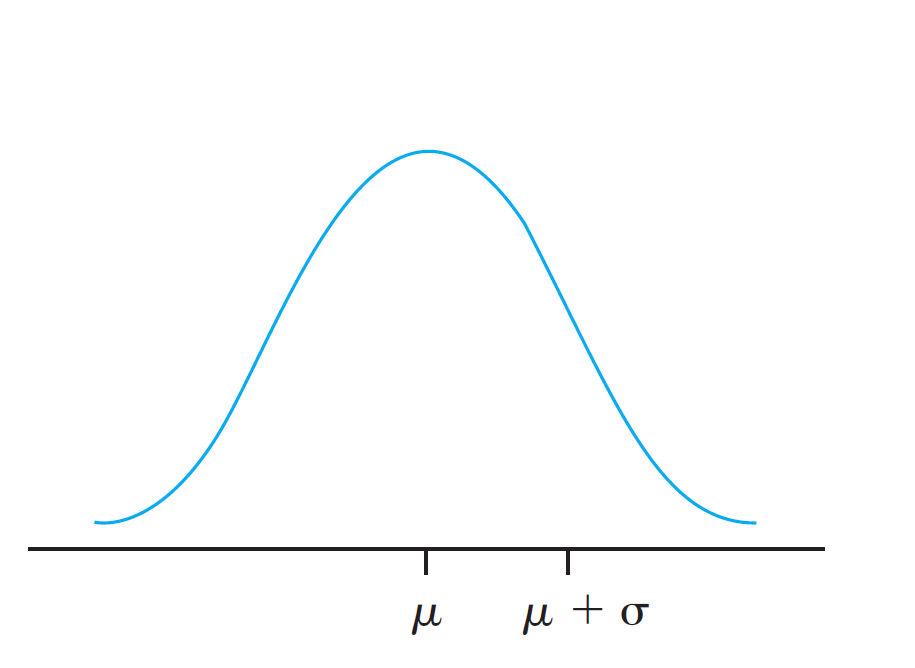
\includegraphics[scale=0.4]{figures/normal_distribution.png}
\caption{Bell-shaped curve}
\end{figure}
Symmetric about $\mu$, $\mu$=shift, $\sigma$=scale, large $\sigma\Rightarrow$large spread out.
 
\begin{prop}
Properties
\begin{enumerate}
\item $E(X)=\mu \qquad	Var(X)=\sigma^2$
\item $f(x) \to 0$, when $x \to \pm \infty$
\end{enumerate}
\end{prop}

\subsection{The Standard Normal Distribution}
The Standard Normal Distribution, $N(0,1)$, denoted by $Z$,
\[f(x)=\frac{1}{\sqrt{2 \pi}} e^{-\frac{x^2}{2}}  \qquad -\infty< x< \infty\]
c.d.f of $Z$
\[\Phi(x)=\int_{-\infty}^{\infty} \frac{1}{\sqrt{2 \pi}} e^{-\frac{x^2}{2}}  dx\]
\begin{align*}
&\Phi(0)=0.5 \\
&\Phi(1.645)=0.95 \qquad \Phi(1.96)=0.975 \\
&\Phi(-1.645)=0.05 \qquad \Phi(-1.96)=0.025
\end{align*}

\begin{exmp}
(1)
\begin{align*}
&P(-1.645 \leq Z \leq 1.96)\\
=&P(Z \leq 1.96)-P(Z \geq -1.645) \\
=&\Phi(1.96)-\Phi(-1.645)=0.975-0.05=0.925
\end{align*}

(2)
\begin{align*}
&P(-0.38 \leq Z \leq 1.25)\\
=&\Phi(1.25)-\Phi(-0.38)=0.8944-(1-\Phi(0.38))\\
=&0.8944-(1-0.6486)=0.5424
\end{align*}
\end{exmp}

\subsubsection{Using Standard Normal Table}

\subsection{Percentiles of the Standard Normal Distribution}
$100p$ th percentile $\eta_{p}$ of $X$ is the solution of 
\[F(\eta_p)=p\]

\begin{exmp}
For $Z$
\[\eta_{0.975}=1.96 \qquad \eta_{0.95}=1.645\]
\[\eta_{0.025}=-1.96 \qquad \eta_{0.05}=-1.645\]
\[\eta_{0.9}=1.28\]
\end{exmp}


\subsection{$z_{\alpha}$ Notation for $z$ Critical Values}
$z_{\alpha}$ will denote the value on the $z$ axis for which $\alpha$ of the area under the $z$ curve lies to the right of $z$. 
\[z_{0.05}=\eta_{0.95}=1.645\]
(lower percentile)
\subsection{Nonstandard Normal Distributions}
If $X \sim N(\mu,\sigma^2) $,then
\[Z=\frac{X-\mu}{\sigma} \sim N(0,1)\]
\begin{align*}
P(a\leq X\leq b) &= P \left(\frac{a-\mu}{\sigma} \leq \frac{X-\mu}{\sigma} \leq \frac{b-\mu}{\sigma} \right)  \\
& = P \left( \frac{a-\mu}{\sigma} \leq Z \leq \frac{b-\mu}{\sigma} \right) =\Phi \left(\frac{b-\mu}{\sigma} \right)- \Phi \left(\frac{a-\mu}{\sigma} \right)
\end{align*}
Similarly,
\begin{align*}
P(X\leq a) &= P \left(\frac{X-\mu}{\sigma} \leq \frac{a-\mu}{\sigma} \right)  \\
& = P \left(  Z \leq \frac{a-\mu}{\sigma} \right) =\Phi \left(\frac{a-\mu}{\sigma} \right)
\end{align*}
\[P(X \geq b)=1-\Phi \left(\frac{b-\mu}{\sigma} \right)\]

\begin{exmp}
$X \sim N(1.25,0.46)$
\begin{align*}
P(1 \leq X\leq 1.75) &= P \left(\frac{1-1.25}{\sqrt{0.46}} \leq \frac{X-1.25}{\sqrt{0.46}} \leq \frac{1.75-1.25}{\sqrt{0.46}} \right)  \\
& = P \left( -0.369 \leq Z \leq 0.737 \right)\\
&=\Phi \left(0.737 \right)- \Phi \left(-0.369 \right)=\boxed{0.4147}
\end{align*}
\end{exmp}

\subsection{Empirical Rule}
If a population distribution of a r.v is roughly normal. Then
\begin{enumerate}
\item 68\% of the values are within 1 s.d of their mean.
\item 95\% of the values are within 2 s.d of their mean.
\item 99.7\% of the values are within 3 s.d of their mean.
\end{enumerate}
\begin{proof}
\begin{align*}
LHS=&P(\mu-\sigma \leq X \leq \mu+\sigma)=P(-1 \leq\frac{X-\mu}{\sigma}\leq 1)\\
=&\Phi(1)-\Phi(-1)=0.8413-(1-0.8413)=68.26\%
\end{align*}
\end{proof}

\subsection{Percentiles of an Arbitrary Normal Distribution}
If $X\sim N(\mu,\sigma^2)$ c.d.f $F(x)$, (100$p$)th percentile of $X$ is the root of 
\begin{align*}
P=F(\eta_p)=&P(X \leq \eta_p)\\ 
=&P\left(\frac{X-\mu}{\sigma} \leq \frac{\eta_p-\mu}{\sigma} \right)=\Phi\left( \frac{\eta_p-\mu}{\sigma} \right)
\end{align*}
So,$\frac{\eta_p-\mu}{\sigma}$ is the $(100p)$th percentile of $N(0,1)$. Therefore, $(100p)$th percentile of $N(\mu,\sigma^2)$=$\mu+\sigma\times[100p\text{th percentile of }N(0,1)]$

\begin{exmp}
$X \sim N(64,0.78^2)$. Then 99.5 percentile of $X$ is $64+0.78\times 2.58=66$, where 2.58 is the 99.5 percentile of $Z$. 
\end{exmp}

\subsection{Approximating the Binomial Distribution}
If $X \sim Binom(n,p)$. When $n$ is large, and $p$ is not too small or too large, s.t. $np \geq 10, n(1-p) \geq 10$. Then $X \sim N(np,np(1-p))$
\[p(x)=\binom nx p^x (1-p)^{n-x} \qquad x=0,1,\dots,n\]


$X \sim Binom(n,p)$\footnote{$X \sim N(np,np(1-p))$, to avoid significant deviation},
\begin{align*}
P(a \leq X \leq b)&=P(a-0.5 \leq X \leq b+0.5)  \\
P(X \leq a) &= P(X \leq a+0.5)	\\
P(X \geq b) &= P(X \geq b-0.5)
\end{align*}

\begin{exmp}
25\% of all drivers in HK don't have insurance. Randomly select 50 drivers. $X=$ \# of drivers uninsured.

(1)$P(X \leq 10)$ \quad (2)$P(5 \leq X \leq 15)$ \\
First $X\sim Binom(50,0.25) \dot{\sim} N(12.5,12.5\times1.75)$

(1) \begin{align*}
P(X\leq 10) =& P(X \leq 10.5) \\
=& P\left( \frac{X-12.5}{\sqrt{12.5\times1.75}}  \leq   \frac{10.5-12.5}{\sqrt{12.5\times1.75}}\right)=\Phi(-0.653)=0.2578
\end{align*}

(2) \begin{align*}
P(5 \leq X\leq 15) =& P(4.5 \leq X \leq 15.5) \\
=& P\left(\frac{4.5-12.5}{\sqrt{12.5\times1.75}} \leq \frac{X-12.5}{\sqrt{12.5\times1.75}}  \leq   \frac{15.5-12.5}{\sqrt{12.5\times1.75}}\right)	\\
=&\Phi(0.95)-\Phi(-2.61)=0.832
\end{align*}
\end{exmp}

\section{The Exponential and Gamma Distributions}
\subsection{The Gamma Function}
\begin{defn}
\[\Gamma(\alpha)=\int_0^{\infty} x^{\alpha-1}e^{-x} dx\]
\end{defn}

This function has the following properties:
\begin{enumerate}
\item $\Gamma(\alpha)=(\alpha-1)\Gamma(\alpha-1)$
\item $\Gamma(1)=1,\Gamma(2)=1,\Gamma(3)=2$\\
$\Gamma(n)=(n-1)! \qquad n=1,2,\dots$
\item $\Gamma(\frac{1}{2})=\sqrt{\pi}$
\end{enumerate}

\subsection{The Gamma Distribution}
\begin{defn}
X follows a Gamma distribution. $X \sim Gamma(\alpha,\beta)$
\[f(x)=\begin{cases}
\frac{1}{\Gamma(\alpha)} \frac{1}{\beta^{\alpha}} x^{\alpha-1} e^{-x/\beta}, & \text{if} \quad x\geq 0\\
0. & \text{if} \quad x < 0
\end{cases}\]
for $\alpha>0, \beta>0$
\end{defn}

If $\beta=1$, $X \sim Gamma(\alpha,1)$. Standard Gamma distribution.
\[f(x)=\begin{cases}
\frac{1}{\Gamma(\alpha)}  x^{\alpha-1} e^{-x}, & \text{if} \quad x\geq 0\\
0. & \text{if} \quad x < 0
\end{cases}\]

Check
\[\int_{0}^{\infty}\frac{1}{\Gamma(\alpha)}  \frac{1}{\beta^{\alpha}} x^{\alpha-1} e^{-x/\beta} dx=1\]
\begin{align*}
L.H.S.&=\int_{0}^{\infty}\frac{1}{\Gamma(\alpha)}   u^{\alpha-1} e^{-u} du \\
&=\frac{1}{\Gamma(\alpha)} \int_{0}^{\infty} u^{\alpha-1} e^{-u} du=1
\end{align*}

\begin{prop}
If $X\sim Gamma(\alpha,\beta)$, then $E(X)=\alpha\beta$, $Var(X)=\alpha\beta^2$
\begin{proof}
\begin{align*}
E(X)&=\int_{0}^{\infty}x \frac{1}{\Gamma(\alpha)} \frac{1}{\beta^{\alpha}} x^{\alpha-1} e^{-x/\beta} dx = \frac{1}{\Gamma(\alpha)} \int_{0}^{\infty} \frac{1}{\beta^{\alpha}} x^{\alpha} e^{-x/\beta} dx  \\
&=\frac{\beta}{\Gamma(\alpha)} \int_{0}^{\infty} \frac{1}{\beta^{\alpha+1}} x^{\alpha} e^{-x/\beta} dx =  \frac{\beta \Gamma(\alpha+1)}{\Gamma(\alpha)} \int_{0}^{\infty}\frac{1}{\Gamma(\alpha+1)}  \frac{1}{\beta^{\alpha+1}} x^{\alpha} e^{-x/\beta} dx \\
&=\frac{\Gamma(\alpha+1)}{\Gamma(\alpha)}\beta =\alpha\beta
\end{align*}
\end{proof}
\end{prop}

\begin{exmp}
Suppose that the reaction time $X$ of a randomly selected individual to a certain stimulus has a standard Gamma distribution with $\alpha=2$.
\[P(3 \leq X \leq 5)=F(5;2)-F(3;2)\]
Here $F(x;\alpha)$ is the c.d.f of $\Gamma(\alpha,1)$
\[Table A.4=0.960-0.801=0.159\]
\end{exmp}

\begin{prop}
If $X\sim Gamma(\alpha,\beta)$, then $X/\beta \sim Gamma(\alpha,1)$
\[P(X\leq x)=P\left(\frac{X}{\beta} \leq \frac{x}{\beta}\right)=F\left(\frac{x}{\beta};\alpha \right)\]
\end{prop}

\begin{exmp}
The survival time $X$ of a randomly selected male mouse exposed to gamma radiation has Gamma distribution with $\alpha=8$, $\beta=15$. Then
\[E(X)=\alpha\beta =8 \times 15 =120\]
\[Var(X)=\alpha \beta^2 =8 \times 15^2 =1800\]
\begin{align*}
P(60 \leq X \leq 120)&=P\left(\frac{60}{15}\leq\frac{X}{15} \leq\frac{120}{15} \right)=F(8;8)-F(4;8) \\
&=0.547-0.051=0.496
\end{align*}
\end{exmp}

\subsection{Exponential distribution}
If $X\sim exp(\lambda)$,
$f(x)=\begin{cases}
\lambda e^{-\lambda x}, 	& x >0\\
0. &\text{otherwise}
\end{cases}$. Then $X$ has an exponential distribution with parameter $\lambda$.

\begin{prop}
If $X\sim exp(\lambda)$. Then $X \sim Gamma(1,1/\lambda)$
\[E(X)=\lambda \qquad Var(X)=\frac{1}{\lambda^2}\]
\end{prop}

\begin{exmp}
X=response time at some computer terminal. $X \sim exp(\lambda)$. Suppose that the expected reacting time is 5 seconds.
\[E(X)=5 \qquad \frac{1}{\lambda}=5 \Rightarrow \lambda=\frac{1}{5}\]
\[P(X\leq 10)=\int_0^{10} \frac{1}{5} e^{-x/5} dx=\left. e^{-x/5}\right|_{0}^{10}=1-e^{-2}. \]
\end{exmp}


In general, if $X\sim exp(\lambda)$,
\[F(x)=\int_0^{x} \lambda e^{-\lambda y} dy=\left. e^{-\lambda y}\right|_{0}^{x}=1-e^{-\lambda x}\]

\subsubsection{Two applications}
\textbf{(A)} Suppose \# of customers coming in any wait time $\sim Possion(\alpha)$, and \# of customers is non-overlapping intervals are independent. Then
\[X= \text{the elapsed time between the successive customers coming in}\sim exp(\alpha)\]
Why? Let $X_1$=waiting time before the 1st customer coming in. Want to show that $X_1 \sim exp()\lambda$, just need to find $f_{X_1}(x)$. Then we just need to find $F_{X_1}(x)$, as $f_{X_1}(x)=F'_{X_1}(x)$.
\begin{align*}
F_{X_1}(x)&= P(X_1\leq x)=P(\text{at least 1 customer in }(0,x)) \\
&= 1-P(\text{no customer in }(0,x)) \\
&=1-\frac{(\alpha x)^0}{0!}e^{-\alpha x}=1-e^{-\alpha x}
\end{align*}
\[f_{X_1}(x)=F'_{X_1}(x)=\alpha e^{-\alpha x} \qquad x>0\]
\[X_1 \sim exp(\lambda)\]


\textbf{(B)Memoryless property}

Suppose component lifetime $\sim exp(\lambda)$. Putting this component into work, after $t_0$ time, check it and find it is still working. What is the probability that it will last at least another $t$ time?\\
Let $T$ = lifetime of this component $\sim exp(\lambda)$
\begin{align*}
P(T\geq t_0+t|T \geq t_0)&=\frac{P(T\geq t_0+t \cap T \geq t_0)}{P(T \geq t_0)} \\
&=\frac{P(T\geq t_0+t)}{P(T \geq t_0)}=\frac{1-P(T\leq t_0+t)}{1-P(T \leq t_0)} \\
&=\frac{1-(1+e^{-\alpha(t_0+t)})}{1-(1+e^{-\alpha t_0})}=\frac{e^{-\alpha(t_0+t)}}{e^{-\alpha t_0}} \\
&=e^{-\alpha t}
\end{align*}

\subsection{The Chi-Squared Distribution}
Let $\nu$ be an integer, if $X \sim Gamma(\nu,\frac{\nu}{2})$, then we say $X$ has a $\chi^2$-distribution with parameter $\nu$, $X \sim \chi^2 (\nu)$.

It's p.d.f is
\[f(x;\nu)=\begin{cases}
\frac{1}{2^{\nu/2}\Gamma(\nu/2)} x^{\nu/2-1}e^{-x/2} & x>0 \\
0 & o.w.
\end{cases}\]


\begin{prop}
Properties
\begin{enumerate}
\item If $X \sim N(0,1)$, then $X^2 \sim \chi^2 (1)$
\item If $X_1 \sim \chi^2 (n)$, $X_2 \sim \chi^2 (m)$, independently. Then $X_1+X_2 \sim \chi^2 (m+n)$ 
\item If $X_1 \sim N(0,1)$, $X_2 \sim N(0,1)$, independently. Then $X_1+X_2 \sim \chi^2 (2)$ 
\end{enumerate}
\end{prop}

\section{Other Continuous Distributions}
\subsection{The Weibull Distribution}
If $X \sim Weibull(\alpha,\beta)$
\[f(x)=\frac{1}{\beta^{\alpha}}x^{\alpha-1}e^{-(x/\beta)^{\alpha}} \qquad x >0\]
If $\alpha=1$, $X \sim Weibull(1,\beta)$. Then $X \sim exp(\frac{1}{\beta}) $

\begin{figure}[H]
\centering
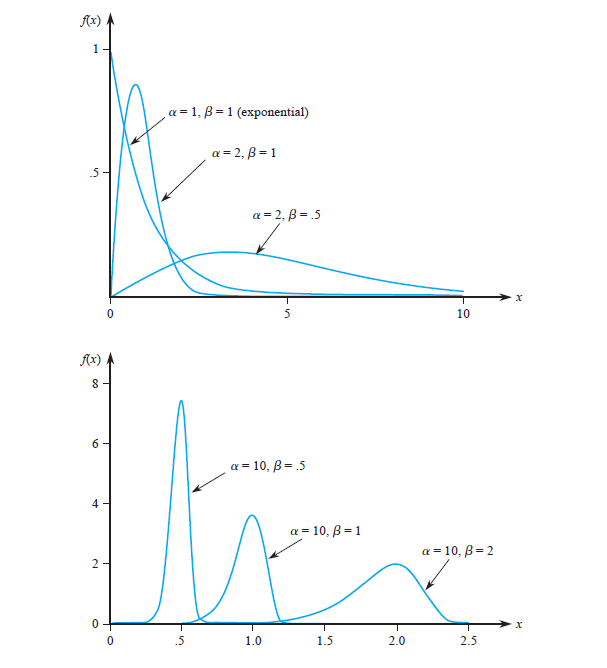
\includegraphics[scale=1]{figures/weibull_distribution.png}
\caption{The Weibull Distribution}
\end{figure}

\begin{prop}
 $X \sim Weibull(\alpha,\beta)$
\begin{enumerate}
\item $E(X)=\beta \Gamma(1+1/\alpha)$
\item $Var(X)=\beta^2\left(\Gamma(1+2/\alpha)-(\Gamma(1+1/\alpha))^2\right)$
\item c.d.f
\[F(x)=\begin{cases}
1-e^{-(\alpha/\beta)^{\alpha}} & x \geq 0 \\
0	&o.w. \\
\end{cases}\]
\end{enumerate}
\end{prop}

\begin{exmp}
$X$ = the strength at  -20 F of a type of steel exhibiting "cold brittleness" at low temperature . $X \sim Weibull(20,100)$

(1) 
\[P(X \leq 105)=F(105)=1-e^{-(105/100)^{20}}=1-0.07=\boxed{0.93}\]
(2)
\[P(90 \leq X \leq 100)=F(110)-F(90)=\left(1-e^{-(110/100)^{20}}\right)-\left(1-e^{-(90/100)^{20}}\right)=\boxed{\dots}\] 
\end{exmp}

\subsection{The Lognormal Distribution}
$X$ is positive. If $\log{X} \sim N(\mu,\sigma^2)$ \footnote{$\log=\ln$} , then $X \sim Lognormal(\mu,\sigma^2)$.
\[f(x)=\frac{1}{\sqrt{2 \pi \sigma^2}} e^{-\frac{(\log{x}-\mu)^2}{2 \sigma^2}}   \qquad  x>0\]
\begin{align*}
E(X)&=e^{\mu +\frac{\sigma^2}{2}} \\
Var(X)&=e^{2\mu +\sigma^2} (e^{\sigma^2}-1)
\end{align*}
\[P(X \leq x)=P(\log{X}\leq \log{x})= P \left(\frac{\log{X}-\mu}{\sigma} \leq \frac{\log{x}-\mu}{\sigma} \right)  =\Phi \left(\frac{\log{x}-\mu}{\sigma} \right)\]

\begin{exmp}
$X$=the modulus of elasticity of some floor system.
\[X \sim Lognormal(0.375,0.25^2)\]
\begin{align*}
E(X)&=e^{0.375+0.25^{2}/2}=1.5\\
Var(X)&= e^{2\times0.375+0.25^{2}}\left(e^{0.25^{2}}-1\right)=0.145\\
P(1 \leq X \leq 2)&=P(\log{1} \leq \log{X}\leq \log{2})\\
&= P \left(\frac{0-0.375}{0.25} \leq \frac{\log{X}-0.375}{0.25} \leq \frac{\log{2}-0.375}{0.25} \right) \\
& =\Phi \left(\frac{\log{2}-0.375}{0.25} \right)-\Phi \left(\frac{-0.375}{0.25} \right)=\boxed{0.8312}
\end{align*}


\end{exmp}

\subsection{The Beta Distribution}
If $X$ has a p.d.f 
\[f(x)=\begin{cases}
\frac{\Gamma(\alpha+\beta)}{\Gamma(\alpha)+\Gamma(\beta)}x^{\alpha-1}(1-x)^{\beta-1}  & 0 \leq x \leq 1 \\
0. & o.w.
\end{cases}\]
Then, $X \sim Beta(\alpha,\beta)$

\begin{prop}
Particularly, if $\alpha=\beta=1$, $X \sim unif(0,1)$
\end{prop}

\begin{prop}
Let $A < B$, and $Y=A+(B-A)X$, then $Y$ be density.
\[f(y)=\begin{cases}
\frac{1}{B-A}\frac{\Gamma(\alpha+\beta)}{\Gamma(\alpha)+\Gamma(\beta)}\left(\frac{y-A}{B-A}\right)^{\alpha-1}\left(\frac{B-y}{B-A}\right)^{\beta-1}  & A \leq x \leq B \\
0. & o.w.
\end{cases}\]
\[Y \sim GBeta\]
\end{prop}

\begin{prop}
If $Y \sim Beta(\alpha,\beta)$
\[E(X)=\frac{\alpha}{\alpha+\beta} \qquad Var(X)=\frac{\alpha\beta}{(\alpha+\beta)(\alpha+\beta+1)}\]
If $Y \sim GBeta(\alpha,\beta,A,B)$
\[E(Y)=A+(B-A)\frac{\alpha}{\alpha+\beta} \qquad Var(Y)=(B-A)^2 \frac{\alpha\beta}{(\alpha+\beta)(\alpha+\beta+1)} \]
Because $Y=A+(B-A)X$, \[E(Y)=E(A+(B-A)X)=A+(B-A)E(X) \qquad Var(Y)=(B-A)^2 Var(X)\]
\end{prop}

\begin{exmp}
\[X=\text{time to complete certain project}\]
\[X \sim GBeta(\alpha=2,\beta=3,A=2,B=5)\]
\[E(X)=2 + (5-2)\frac{2}{2+3}=3.2 \qquad Var(X)=0.36\]
\[P(X \leq 3)=\int_{2}^{3} \frac{1}{5-2}\frac{\Gamma(5)}{\Gamma(2)+\Gamma(3)}\left(\frac{x-2}{3}\right)^{2-1}\left(\frac{5-x}{3}\right)^{3-1} dx=\boxed{0.407}\]
\end{exmp}

\subsection{Challenge Question 2}
Cauchy distribution
\[f(x)=\frac{1}{\pi(1+x^2)}\]
\url{https://en.wikipedia.org/wiki/Cauchy_distribution}
% chapter 5
% Last edit: 2017-4-24
\chapter{Joint Probability Distributions and Random Samples}
\section{Jointly Distributed Random Variables}
\subsection{Two Discrete Random Variables}
$X$,$Y$ are r.v's defined on $\mathcal{S}$. The joint p.m.f is defined as 
\[p(x,y)=P(X=x,Y=y)\]
Let $A$ be an event consisting of pairs of $(x,y)$. Then
\[P\left((X,Y)\in A\right) = \sum_{(X,Y)\in A}p(x,y)\]

\begin{exmp}
Insurance company. For a a newcomer, he has two insurance. Home \& Cars. Deductible amount: Auto \$100, \$250; Home \$0, \$100, \$200.
\begin{center}
\begin{tabular}{c|c|ccc}
\hline
    &     &    & $Y$ &   \\
\hline
    & $p(x,y)$ & 0    & 100  & 200  \\
$X$ & 100      & 0.2  & 0.1  & 0.2  \\
    & 250      & 0.05 & 0.15 & 0.3  \\
\hline
\end{tabular}
\end{center}
An individual home-owner is randomly selected.
\begin{align*}
P(Y \geq 100)=& P(X=100, Y=100)+P(X=250, Y=100)+P(X=100, Y=200)+\\
&P(X=250, Y=200)\\
=& 0.1+0.15+0.2+0.3=0.75
\end{align*}
\end{exmp}

\begin{defn}
"Marginal" p.m.f of $X$ and $Y$, denoted by $p_X(x)$ and $p_Y(y)$ respectively, are given by
\begin{align*}
p_X(x)&=\sum_{y}p(x,y)	\\
p_Y(y)&=\sum_{x}p(x,y)	\\
p_X(x)&=P(X=x)=P(X+x,Y=\dots)+\dots
\end{align*}
\end{defn}

\begin{exmp}
In the Insurance example,
\[P(X=x)=\begin{cases}
P_X(100)=\dots=0.5\\
P_X(250)=\dots=0.5\\
\end{cases}\]
\[P(Y=y)=\begin{cases}
P_Y(0)=\dots=0.25 \\
P_Y(100)=\dots=0.25\\
P_Y(200)=\dots=0.5\\
\end{cases}\]
\end{exmp}
\begin{center}
\begin{tabular}{c|c|ccc|c}
\hline
    &     &    & $Y$ &   & \\
\hline
    & $p(x,y)$ & 0    & 100  & 200 & $p_X(x)$  \\
$X$ & 100      & 0.2  & 0.1  & 0.2 & 0.5 \\
    & 250      & 0.05 & 0.15 & 0.3 & 0.5 \\
    \hline
    & $p_Y(y)$ & 0.25 & 0.25 & 0.5 & 1 \\
\hline
\end{tabular}
\end{center}

\subsection{Two Continuous Random Variables}
$(X,Y)$ continuous r.v. $f(x,y)$ is the joint p.d.f of $X$ and $Y$ if for any 2-dimensional set.
\[P((X,Y)\in A)=\iint_{A} f(x,y)\,dx \,dy\]
Particularly for $A =\{(x,y),a \leq x\leq b,c \leq y \leq d\}$,
\begin{align*}
P(A)&=P(a\leq X \leq b,c  \leq Y \leq d)\\
&= \int_{a}^b \int_c^d f(x,y) \,dy \,dx=\int_c^d \int_{a}^b f(x,y) \,dx \,dy
\end{align*}

\begin{exmp}
\begin{align*}
X=&\text{ right front tyre pressure}\\
Y=&\text{ left front tyre pressure}
\end{align*}
\[f(x,y)=\begin{cases}
k(x^2+y^2)   & 20\leq x,y \leq 30\\
0, 		& o.w.
\end{cases}\]
(1) What is $k$?
\begin{align*}
1=& \int_{20}^{30}\int_{20}^{30} k(x^2+y^2) dx dy = k\int_{20}^{30}  \left(\left.\left( \frac{x^3}{3}+xy^2 \right)\right|_{20}^{30} \right)dy \\
=& k \int_{20}^{30}  \left(\frac{19000}{3}+10y^2\right)dy=k\left(\frac{19000}{3}+\frac{19000}{3}\right) \\
&\Rightarrow k=\frac{3}{38000}
\end{align*}
(2)\begin{align*}
P(X\leq 26, Y\leq 26)=& \int_{20}^{26}\int_{20}^{26} k(x^2+y^2) dx dy\\
=&   k \int_{20}^{26}  \left(\frac{26^3-20^3}{3}+6y^2\right)dy\\
=&	2k\cdot 6 \cdot\frac{1}{3} (26^3-20^3)=0.3024
\end{align*}
\end{exmp}

\begin{defn}
Marginal rv
\begin{align*}
f_X(x)&=\int_{-\infty}^{\infty} f(x,y) dy	\\
f_Y(y)&=\int_{-\infty}^{\infty} f(x,y) dx	
\end{align*}
\end{defn}

\begin{exmp}
Example 5.4 (continued)

(3)
\begin{align*}
f_X(x)=& \int_{20}^{30} k(x^2+y^2) dy =k  \left. \left( \frac{y^3}{3}+x^2 y \right)\right|_{20}^{30}  \\
=& k\left(10x^2 +\frac{19000}{3}\right)=\frac{3}{38000}x^2+\frac{1}{20} \qquad 20 \leq x \leq 30
\end{align*}
\[f_Y(y)=\frac{3}{38000}y^2+\frac{1}{20} \qquad 20\leq y \leq 30\]
(4)
\[P(20 \leq X \leq 25)=\int_{20}^{25} f_X(x)dx=\dots=0.45\]

\end{exmp}

\begin{defn}
Expected Values
\[E[h(X,Y)]=\int_{-\infty}^{\infty} \int_{-\infty}^{\infty} h(x,y) f(x,y) dx dy \]
\end{defn}

\begin{exmp}
Example 5.4 (continued)

(5)
\[E(X+Y)=\int_{20}^{26}\int_{20}^{26}(x+y) k(x^2+y^2) dx dy=\dots\]
\end{exmp}

\subsection{Independent Random Variables}
$X$ and $Y$ are said to be independent, if 
\begin{align*}
discrete: p(x,y)&=p_X(x)p_Y(y) \text{ for all }(x,y)\\
continuous: f(x,y)&=f_X(x)f_Y(y) \text{ for all }(x,y)
\end{align*}

\begin{exmp}
Example 5.4 (continued)

(6)
\begin{align*}
f(x,y) =& \frac{3}{38000} (x^2+y^2) \qquad 20 \leq x,y \leq 30\\
f_X(x) =&  \frac{3}{38000}x^2+\frac{1}{20} \qquad 20 \leq x \leq 30 \\
f_Y(y) =&  \frac{3}{38000}y^2+\frac{1}{20} \qquad 20 \leq y \leq 30
\end{align*}
\[f(x,y)\neq f_X(x)f_Y(y) \qquad \text{for } x=20, y=20\]
$X$ and $Y$ are not independent. 
\end{exmp}

\begin{exmp}
\[f(x,y)=\lambda_1\lambda_2 e^{-\lambda_1 x - \lambda_2 y}, x\geq0,y\geq0\]
Are $X$ and $Y$ independent?
\begin{align*}
f_X(x)&=\int_{0}^{\infty} \lambda_1 \lambda_2 e^{-\lambda_1 x-\lambda_2 y} dy \\
&=\lambda_1 e^{-\lambda_1 x} \int_{0}^{\infty} \lambda_2 e^{-\lambda_2 y} dy = \lambda_1 e^{-\lambda_1} \qquad x \geq 0
\end{align*}
\[f_Y(y)=\lambda_2 e^{-\lambda_2} \qquad y \geq 0\]
\[f(x,y)= f_X(x)f_Y(y) \qquad \text{for any } (x,y)\]
So, $X \!\perp\!\!\!\perp Y$.
\end{exmp}


\subsection{More Than Two Random Variables}
\begin{defn}
$X_1,X_2,\dots,X_n$ are discrete rvs', the joint p.m.f is defined as
\[p(x_1,x_2,\dots,x_n)=P(X_1=x_1,\dots ,X_n=x_n)\]
In continuous case, the joint p.d.f $f(x_1,x_2,\dots,x_n)$ is such that
\[P(A) =\int_A\dots\int f(x_1,x_2,\dots,x_n) d x_n \dots d x_1\]
\end{defn}

Particularly, $A=\{a_1\leq x_1 \leq b_1,\dots,a_n\leq x_n \leq b_n\}$
\begin{align*}
P(A)=&P(a_1\leq x_1 \leq b_1,\dots,a_n\leq x_n \leq b_n)\\
&=\int_{a_1}^{b_1}\dots\int_{a_n}^{b_n} f(x_1,x_2,\dots,x_n) d x_n \dots d x_1
\end{align*}

\begin{exmp}
A dice is rolled 100 times. $X_i=$\# of $i$ dots out of 100 times; $i=1,2,\dots,6$
\[p_i=P(i \text{ dots}) \qquad p_1+p_2+\dots+p_6=1\]
\[P(X_1=x_1,\dots,X_6=x_6)=\frac{100!}{x_1!x_2!\dots x_6!}p_1^{x_1}p_2^{x_2}\dots p_6^{x_6} \quad(0\leq x_1,\dots,x_6 \leq 100, x_1+\dots+x_6=100)\]
\end{exmp}

\begin{exmp}
$(X_1,X_2,X_3)$ has the joint p.d.f
\[f(x_1,x_2,x_3)=\begin{cases}
kx_1 x_2(1-x_3)   & 0\leq x_1,x_2,x_3 \leq 1,x_1+x_2+x_3\leq 1\\
0, 		& o.w.
\end{cases}\]
(1) What is $k$?
\begin{align*}
1&=\iiint kx_1 x_2(1-x_3) \,dx_3 \,dx_2 \,dx_1 \\
&=\int_0^1 \int_0^{1-x_1} \int_{0}^{1-x_2-x_1} kx_1 x_2(1-x_3) \,dx_3 \,dx_2 \,dx_1 \\
&= \frac{k}{144} \Rightarrow k=144
\end{align*}
(2)
\begin{align*}
P(X_1+X_2 \leq 0.5)=\iiint kx_1 x_2(1-x_3) \,dx_3 \,dx_2 \,dx_1 =0.606
\end{align*}
$0\leq x_1,x_2,x_3 \leq 1, x_1+x_2 \leq 0.5$ \footnote{The value might be wrong, run this in Mathematica -\texttt{ Integrate[144*x y (1 - z), \{x, 0, 0.5\}, \{y, 0, 0.5 - x\}, \{z, 0, 1 - x - y\}]} }
\end{exmp}

\subsubsection{Independence}
\begin{defn}
$X_1,X_2,\dots,X_n$ are independent if 
\[p(x_1,x_2,\dots,x_n)=p_{X_1}(x_1)\dots p_{X_n}(x_n)\]
or
\[f(x_1,x_2,\dots,x_n)=f_{X_1}(x_1)\dots f_{X_n}(x_n)\]
for all possible $(x_1,\dots,x_n)$
\end{defn}

\subsection{Conditional Distributions}

\begin{defn}
$(X,Y)$ with $f(x,y),f_X(x),f_Y(y)$, then the conditional p.d.f of $Y$ given $X=x$,
\[f_{Y|X}(y|x)=\frac{f(x,y)}{f_X(x)}\]
for discrete case
\[p_{Y|X}(y|x)=\frac{p(x,y)}{p_X(x)}\]
\end{defn}

\begin{exmp}
\[f(x,y)=\begin{cases}
\frac{6}{5} (x+y^2) & 0\leq x\leq 1,0\leq y\leq 1 \\
0 & o.w.
\end{cases}\]
\begin{align*}
f_X(x)=& \int_0^1 \frac{6}{5} (x+y^2) \,dy = \left.\left( \frac{6}{5}xy +\frac{6}{5}\frac{1}{3}y^3\right)\right|_0^1\\
=& \frac{6}{5} x +\frac{2}{5}. \qquad 0\leq x \leq 1 
\end{align*}
\[f_{Y|X}(y|0.8)=\frac{f(0.8,y)}{f_X(0.8)}=\frac{15}{17}y^2+\frac{12}{17} \qquad 0\leq y \leq 1 \]
\[E(Y|X=0.8)=\int_0^1 y f_{Y|X}(y|0.8) \,dy=\int_0^1 y\left(\frac{15}{17}y^2+\frac{12}{17}\right)\,dy=\frac{39}{68}\]
\end{exmp}

\section{Expected Values, Covariance, and Correlation}
\begin{prop}
\[E[h(x,y)]=\begin{cases}
\sum_{x}\sum_{y} h(x,y)p(x,y) & discrete \\
\int_{-\infty}^{\infty} \int_{-\infty}^{\infty} h(x,y) f(x,y) dx dy & continuous
\end{cases}\]
\end{prop}

\begin{exmp}
\begin{align*}
X &= \text{amount of almonds}\\
Y &= \text{amount of pecans}
\end{align*}
\[f(x)=
\begin{cases}
24xy & \text{if }0\leq x,y\leq1, x+y\leq1\\
0 & o.w. 
\end{cases}\]
Unit test: almonds: \$1.00; pecans: \$1.00; peanuts: \$ 0.50
\[h(X,Y)=X+1.5Y+0.5(1-X-Y)=0.5+0.5X+Y\]
\[E[h(x,y)]=\int_{0}^{1} \int_{0}^{1-y}(0.5+0.5x+y)24xy \,dx \,dy=1.10\]
\end{exmp}

\subsection{Covariance}
\begin{defn}
\[Cov(X,Y)=E\Big((X-\mu_X)(Y-\mu_Y)\Big)\]
where $\mu_X=E(X)$,$\mu_Y=E(Y)$
\[\Rightarrow Cov(X,Y)=E(XY)-E(X)E(Y)\]
\end{defn}

\begin{exmp}
In Example 5.1
\begin{center}
\begin{tabular}{|c|c|ccc|c|}
\hline
    &     &    & $Y$ &   & \\
\hline
    & $p(x,y)$ & 0    & 100  & 200 & $p_X(x)$  \\
$X$ & 100      & 0.2  & 0.1  & 0.2 & 0.5 \\
    & 250      & 0.05 & 0.15 & 0.3 & 0.5 \\
    \hline
    & $p_Y(y)$ & 0.25 & 0.25 & 0.5 & 1 \\
\hline
\end{tabular}
\end{center}
\begin{align*}
E(X)&=100\times 0.5+ 250 \times 0.5= 175 \\
E(Y)&=\dots= 125 \\
Cov(X,Y)&=\dots=1875
\end{align*}
\end{exmp}

\begin{exmp}
\[f(x)=
\begin{cases}
24xy & \text{if }0\leq x,y\leq1, x+y\leq1\\
0 & o.w. 
\end{cases}\]
\[Cov(X,Y)=E(XY)-E(X)E(Y)\]
\[f_X(x)=\int_0^{1-x}\]
Similarly,
\[f_Y(y)=12y(1-y)^2,0\leq y\leq 1\]
\begin{align*}
E(X)&=\int_0^1 x \cdot 12x(1-x)^2 dx =\frac{2}{5}\\
E(Y)&=\frac{2}{5}\\
E(XY)&=\int_0^1  \left(\int_0^{1-y} xy \cdot 24xy \,dx\right)\,dy =\frac{2}{15}\\
Cov(X,Y)&=E(XY)-E(X)-E(Y)=-\frac{2}{75}
\end{align*}
$X,Y$ are negatively related. But Covariance cannot indicate the relation is strong or weak.
\end{exmp}

\subsection{Correlation}
\begin{defn}
The correlation coefficient of $X$ and $Y$, denoted by $Corr(X, Y)$, $\rho_{X,Y}$, or just $\rho$, is defined by
\[Corr(X,Y)=\frac{Cov(X,Y)}{\sqrt{Var(X)Var(Y)}}\]
\end{defn}

Back to Example 5.21,
\[Var(X)=E(X^2)-{E(X)}^2\]
\[E(X^2)=\int_0^1 x^2 12x (1-x)^2 \,gx= 12\int_0^1 x^3 (1-x)^2 \,dx=\frac{1}{5}\]
\[Var(X)=\frac{1}{5}-\left(\frac{2}{5}\right)=\frac{1}{25}\]
Similarly, \[Var(Y)=\frac{1}{25}\]
\[Corr(X,Y)=\frac{-\frac{2}{75}}{\sqrt{\frac{1}{25}\frac{1}{25}}}=-\frac{2}{3}\]

\begin{prop}
\textbf{Fact}: for any $X$ and $Y$,
\[-1\leq Corr(X,Y)\leq 1\]
\end{prop}

\begin{prop}
If $ac >0$\footnote{$a$ and $c$ are either both positive or negative}, then
\[Corr(aX+b,cX+d)=Corr(X,Y)\]
"unit free" 
\end{prop}

\begin{prop}
\begin{enumerate}
\item If $X$ and $Y$ are independent,then
\[Corr(X,Y)=0\]
But $Corr(X,Y)=0 \not\Rightarrow$ $X$ and $Y$ are independent.
\item If $Corr(X,Y)=1$ or $-1$ if and only if $Y=aX+b$ for some $a,b$ with $a \neq 0$.
\end{enumerate}
\end{prop}

\begin{exmp}
$X$ and $Y$ are discrete r.v.'s
\[p(x,y)=\begin{cases}
\frac{1}{4} &(x,y)=(-4,1),(4,-1),(2,2),(-2,-2)\\
0 & o.w.
\end{cases}\]
\[p_X(x)=\begin{cases}
\frac{1}{4} &x=-4,-2,2,4\\
0 & o.w.
\end{cases}\]
\[p_Y(y)=\begin{cases}
\frac{1}{4} &y=-2,-1,1,2\\
0 & o.w.
\end{cases}\]
\[E(X)=\frac{1}{4}(-4+-2+2+4)=0 \qquad E(Y)=0\]
\[E(XY)=\frac{1}{4}(-4+-4+4+4)=0\]
\[Cov(X,Y)=0-0\times0=0 \qquad Corr(X,Y)=0\]
But $X  \not\!\perp\!\!\!\perp Y$.
\end{exmp}

\begin{exmp}
$X \sim N(0,1)$, $Y=X^2 \sim \chi^2 (1)$
\[E(X)=0 \qquad E(Y)=E(X^2)=(Var(X))=1\]
\[E(XY)=E(X^3)=\int_{-\infty}^{\infty}x^3 \phi(x)\,dx=0\]
\[Cov(X,Y)=E(XY)-E(X)E(Y)=0-0\times1=0\]
\[Cov(X,Y)=0 \qquad X  \not\!\perp\!\!\!\perp Y\]
\end{exmp}

\subsection{Properties (The Distribution of a Linear Combination)}
\begin{prop}
\textbf{(1)}. $X_1,X_2 \dots X_n$ are rv's. For any constant $a_1,a_2 \dots a_n$,
\begin{align*}
E(a_1 X_1+\dots+a_n X_n)&=a_1E(X_1)+\dots +a_n E(X_n)\\
Var(a_1 X_1+\dots+a_n X_n)&=\sum_{i=1}^n a_i^2 Var(X_i)+\sum_{i\neq j} a_i a_j Cor(X_i,Y_j)\\
&=\sum_{i=1}^n a_i^2 Var(X_i)+2\sum_{i=1}^{n}\sum_{j=i+1}^{n} a_i a_j Cor(X_i,Y_j)
\end{align*}
If $X_1,X_2 \dots X_n$ are independent
\[Var(a_1 X_1+\dots+a_n X_n)=\sum_{i=1}^n a_i^2 Var(X_i)\]
\[Var(X)=Cov(X,X)=E(XX)-E(X)E(X)\]

\textbf{(2)}. If $X_1,X_2 \dots X_n$ are independent, and $X_i\sim N(\mu_i,\sigma_i^2)$. Then
\[a_1 X_1+\dots+a_n X_n \sim N(\sum_{i=1}^{n} a_i \mu_i,\sum_{i=1}^{n} a_i \sigma^2)\]
Particularly, if $\mu_i=\mu, \sigma_i=\sigma ,a_i=\frac{1}{n}(i=1,\dots,n)$, then
\[\bar{X} \sim N(\mu,\frac{\sigma^2}{n})\]
\end{prop}

\section{Statistics and Their Distributions}
\begin{exmp}
Number of certificate obtained by students: 2,1,4,2,0. 

Sample mean: $\bar{x}=\frac{2+1+4+2+0}{5}=1.8$

Sample variance: $s^2=\frac{(2-1.8)^2+(1-1.8)^2+(4-1.8)^2+\dots}{4}$

Generally, $x_1,x_2,\dots,x_n$,

Sample mean:\[\bar{x}=\frac{x_1+\dots+x_n}{n}\]

Sample variance:\[s^2=\frac{\sum_{i=1}^n (x_i-\bar{x})^2}{n-1}\]
\end{exmp}


\begin{defn}
A statistic is a function of data before sampling (or before data are observed). There is an uncertainty on what value the statistic will result.

Usually, we use upper-case letter to denote statistic, and lower-case letter to denote observe values of a statistic.
\[\bar{X}= \frac{X_1+\dots+X_n}{n} \qquad S^2=\frac{\sum (X_i-\bar{X})^2}{n}\]
$\bar{x},s^2$. $T=\frac{\bar{X}}{S}$ is also a statistic.
\end{defn}


\subsection{Random Samples}
\begin{defn}
$X_1,X_2 \dots X_n$ are said to be a random sample of size $n$ if they are independent and identically distributed (i.i.d).
\end{defn}

\subsection{Deriving the Sampling Distribution of a Statistic}
\begin{exmp}
A car dealer, tune-up charge (\$40,\$45,\$50) for (4,6,8) cylinder cars. At a particular day, of all tune-up cars, (20\%, 30\%, 50\%) are (4,6,8) cylinder cars.

The pmf of revenue is

\begin{center}
\begin{tabular}{l|c|c|c}
\hline
$x$ & 40 & 45 & 50\\
\hline
$p(x)$ & 0.2 & 0.3 & 0.5 \\
\hline
\end{tabular}
\end{center}
\[E(X)=46.5 \qquad Var(X)=15.25\]
At another day, two tune-ups are done.
\begin{align*}
X_1&=\text{revenue for the 1st car}\\
X_2&=\text{revenue for the 2nd car}
\end{align*}
Then $X_1, X_2$ iid $X$ with pmf $p(x)$, $\bar{X}=\frac{X_1+X_2}{2}$.
\begin{center}
\begin{tabular}{l|l|c|c|c}
\hline
$x_1$ &$x_2$ & $p(x_1,x_2)$ & $\bar{x}$ & $s^2$\\
\hline
40 & 40 & 0.04 & 40 & 0 \\
\hline
40 & 45 & 0.06 & 42.5 & 12.5 \\
\hline
40 & 50 & 0.10 & 45 & 50 \\
\hline
45 & 40 & 0.06 & 42.5 & 12.5 \\
\hline
45 & 45 & 0.09 & 45 & 0 \\
\hline
45 & 50 & 0.15 & 47.5 & 12.5 \\
\hline
50 & 40 & 0.10 & 45 & 50 \\
\hline
50 & 45 & 0.09 & 47.5 & 12.5 \\
\hline
50 & 50 & 0.25 & 50 & 0 \\
\hline
\end{tabular}
\end{center}

Distribution of $\bar{X}$
\begin{center}
\begin{tabular}{l|c|c|c|c|c}
\hline
$\bar{x}$ & 40 & 42.5 & 45 & 47.5 & 50\\
\hline
$p_{\bar{X}}(\bar{x})$ & 0.04 & 0.12 & 0.29 & 0.3 & 0.25 \\
\hline
\end{tabular}
\end{center}

Distribution of $S^2$
\begin{center}
\begin{tabular}{l|c|c|c}
\hline
$s^2$ & 0 & 12.5 & 50\\
\hline
$p_{S^2}(s^2)$ & 0.38 & 0.42 & 0.20 \\
\hline
\end{tabular}
\end{center}
\begin{align*}
E(\bar{X})=& 46.5 \\
E(S^2)=& 15.25 = Var(X) \\
Var(S^2)=&
\end{align*}
\end{exmp}

\begin{exmp}
(Example 5.21 in the textbook)
$X_1,X_2 \overset{iid}{\sim}exp(\lambda)$
\[f(x)=\begin{cases}
\lambda e^{-\lambda x}, 	& x >0\\
0. &\text{otherwise}
\end{cases}\]
$Y=X_1+X_2$ is the statistic of interest. $f_Y(y)=?$.
\begin{align*}
F_Y(y)=&P(Y \leq y)=P(X_1+X_2\leq y) \\
=&\iint_{X_1+X_2\leq y} f(x_1,x_2) \,dx_1 \,dx_2 =\int_0^y \int_0^{y-x_2} \lambda e^{-\lambda x_1} \lambda e^{-\lambda x_2} dx_1 \, dx_2 \\
=& \int_0^y \int_0^{y-x_2} \lambda^2 e^{-\lambda(x_1+x_2)} dx_1 \, dx_2= \dots = 1-e^{-\lambda y}- \lambda y e^{-\lambda y} \qquad 0\leq y \leq \infty
\end{align*}
\[f_Y(y)=F'_Y(y)=\lambda e^{-\lambda y} -\lambda e^{-\lambda y}+\lambda^2 y e^{-\lambda y} =\lambda^2 y e^{-\lambda y} \qquad y \geq 0 \]
\[Y\sim Gamma(2,\frac{1}{\lambda})\]
\[E(Y)=\frac{2}{\lambda} \qquad Var(Y)=\frac{2}{\lambda^2}\]
\end{exmp}

\section{The Distribution of the Sample Mean}
\begin{prop}
Let $X_1, X_2, \dots , X_n$ be a random sample from a distribution with mean $\mu$ and variance $\sigma^2$. Then 
\[E(\bar{X})=\mu \qquad  Var(\bar{X})=\frac{\sigma^2}{n} \qquad s.d(\bar{X})=\frac{\sigma}{\sqrt{n}}\]
If $T=X_1+ X_2+ \dots + X_n$,
\[E(T)=n \mu \qquad  Var(T)=n\sigma^2 \qquad s.d(T)=\sqrt{n}\sigma\]
\end{prop}

\subsection{The Case of a Normal Population Distribution}
\begin{exmp}
In a previous class of MA2506, students' final exam score $\sim N(70,20^2)$. This year, the same class, 36 students.
\[\bar{X}=\text{ average score}\]
\[P(65 \leq \bar{X} \leq 75)\]
Since $X_1, X_2, \dots , X_n \overset{iid}{\sim}(70,20^2)$, 
$\bar{X}\sim N(70,\frac{20^2}{36})$
\[P(65 \leq \bar{X} \leq 75)=P\left(\frac{65-70}{20/6} \leq \frac{\bar{X}-70}{20/6} \leq \frac{75-70}{20/6}\right)=\Phi(-1.5 \leq Z \leq 1.5)=0.8664\]
\end{exmp}

\subsection{The Central Limit Theorem}
What if $X_1, X_2, \dots , X_n \overset{iid}{\sim}(\mu,\sigma^2)$? No normality.
\begin{theo}
\textbf{The Central Limit Theorem(CLT)}

Let $X_1, X_2, \dots , X_n$ be a random sample from a distribution with mean $\mu$ and variance $\sigma^2$. Then if $n$ is sufficiently large, $\bar{X}$ has approximately a normal distribution with $\mu_{\bar{X}}=\mu$ and $\sigma_{\bar{X}}=\frac{\sigma^2}{n}$, and $T$ also has approximately a normal distribution with $\mu_{T}=n \mu$, $\sigma_{T}^2=n \sigma^2$. The larger the value of $n$, the better the approximation. Usually, $n \geq 30$.
\end{theo}
% chapter 6
% Last edit: 2017-4-27
\chapter{Point Estimation}
\section{Some General Concepts of Point Estimation}
\begin{exmp}
Population $N(\mu,1)$.
\[10.2, 9.8, 9.5, 11, 13, 9\]
A "guess" of $\mu$ can be $\frac{10.2+9.8+9.5+11+13+9}{6}=10.4$
\end{exmp}

\begin{defn}
Generally, we need to estimate a parameter $\theta$ based on a sample data set $x_1,x_2,\dots,x_n$. A point estimate of $\theta$ is a suitable statistic on $X_1,X_2,\dots,X_n$.
\end{defn}

\begin{exmp}
(Example 6.1 in textbook)
% An unfinished exmp!!
\end{exmp}

\begin{exmp}
(Example 6.2 in textbook)
% An unfinished exmp!!
\end{exmp}

\subsection{Unbiased Estimators}
\begin{defn}
An estimate $\hat{\theta}$ is said to be unbiased if
\[E(\hat{\theta})=\theta\]
Otherwise $E(\hat{\theta})-\theta$ is called the bias of $\hat{\theta}$.
\end{defn}

\begin{exmp}
$X \sim Bin(n,p)$, $\hat{p}=\frac{X}{n}$
\[E(\hat{p})=E\left(\frac{X}{n}\right)=\frac{1}{n}E(X)=p\]
So $\hat{p}$ is an unbiased estimate of $p$.
\end{exmp}

\begin{exmp}
$X_1,\dots,X_n \overset{iid}{\sim} (\mu,\sigma^2)$
\[\hat{\mu}=\bar{X} \qquad \hat{\sigma^2}=\frac{1}{n-1}\sum_{i=1}^n(X_i-\bar{X})^2\]
\[E(\hat{\mu})=E(\frac{X_1+\dots+X_n}{n})=\frac{1}{n}E(X_1+\dots+X_n)\]
\begin{align*}
E(a_1 X_1+\dots+a_n X_n)&=a_1E(X_1)+\dots +a_n E(X_n)\\
Var(a_1 X_1+\dots+a_n X_n)&=\sum_{i=1}^n a_i^2 Var(X_i) \qquad \text{ if }X_1,\dots,X_n \text{ are independent  }  
\end{align*}

\begin{align*}
\Rightarrow E(\hat{\mu})&=\frac{1}{n}(E(X_1)+\dots+E(X_n))=\frac{1}{n}(\mu+\dots+\mu)=\mu \\
 E(S^2)&= E\left(\frac{\sum_{i=1}^n(X_i-\bar{X})^2}{n-1}\right)= \frac{1}{n-1} E\left(\sum_{i=1}^n (X_i^2 -2X_i \bar{X}+\bar{X}^2) \right) \\
 &= \frac{1}{n-1} E\left( \left(\sum_{i=1}^n X_i^2 \right) - n \bar{X}^2 \right) = \frac{1}{n-1} \left( \sum_{i=1}^n E ( X_i^2 ) - n E(\bar{X}^2) \right)
\end{align*}
Recall: $Var(X_i)=E(X_i^2)-(E(X_i))^2, E(X_i)=\mu, Var(X_i)=\sigma^2$ in normal distribution. $\Rightarrow E(X_i^2)=\mu^2+\sigma^2$. $Var(\bar{X})=E(\bar{X}^2)-(E(\bar{X}))^2 \Rightarrow E(\bar{X}^2)=\mu^2 +\frac{\sigma^2}{n}$.
\[E(S^2)=\frac{1}{n-1} \left( \sum_{i=1}^n (\mu^2+\sigma^2) - n \left(\mu^2 +\frac{\sigma^2}{n}\right) \right)=\sigma^2 \]
So, $S^2=\frac{1}{n-1}\sum_{i=1}^n(X_i-\bar{X})^2$ is an unbiased estimate of $\sigma^2$. If we use $\frac{1}{n}\sum_{i=1}^n(X_i-\bar{X})^2$, would generate a bias.
\end{exmp}

\begin{exmp}
(Example 6.4 in textbook)
% An unfinished exmp!!
\end{exmp}

\begin{prop}
If $X_1, X_2,\dots, X_n$ is a random sample from a distribution with mean $\mu$, then $\bar{X}$ is an unbiased estimator of $\mu$. If in addition the distribution is continuous and symmetric, then $\tilde{X}$ (Sample median) and any trimmed mean are also unbiased estimators of $\mu$.
\end{prop}

\subsection{Estimators with Minimum Variance}
\noindent\fbox{%
    \parbox{\textwidth}{%
        \textbf{Principle of Minimum Variance Unbiased Estimation} 
        
        Among all estimators of $\theta$ that are unbiased, choose the one that has minimum variance. The resulting is called the minimum variance unbiased estimator (MVUE) of $\theta$.
    }%
}

\begin{exmp}
(Example 6.6 in textbook)

% An unfinished exmp!!
\end{exmp}

\begin{theo}
$X_1,\dots,X_n \overset{iid}{\sim} N(\mu,\sigma^2)$, then $\hat{\mu}=\bar{X}$ is the MVUE of $\mu$.
\end{theo}

\section{Methods of Point Estimation}
\subsection{The Method of Moments}
\begin{defn}
$X_1,\dots,X_n$ random sample. \\
$k$-th sample moment:
\[\frac{1}{n}\sum_{i=1}^n X_i^k\]
$k$-th population moment:
\[E(X^k)\]
\end{defn}

\begin{defn}
Point estimation: use $\frac{1}{n}\sum_{i=1}^n X_i^k \to E(X^k)$
\end{defn}

\begin{exmp}
$X_1,\dots,X_n \overset{iid}{\sim} N(\mu,\sigma^2)$
\[E(X)=\mu \qquad E(X^2)=(E(X))^2+Var(X)=\mu^2+\sigma^2\]
\begin{align*}       %方程组开始
\left  \{              %方程组的左边包括大括号\{
\begin{array}{ll}     %设定列阵的格式:{lll}是三个L,表示三列的对齐方式为Left对齐
\hat{\mu}=\frac{1}{n}\sum_{i=1}^n X_i \\    %$——分隔列的标记,\\——表示换行
\hat{\mu^2}+\hat{\sigma^2}=\frac{1}{n}\sum_{i=1}^n X_i^2     %$同上
\end{array}           %方程列阵的结束
\right.  \Rightarrow            %方程组的右边无符号,利用“.“来标示
\left  \{              %方程组的左边包括大括号\{
\begin{array}{ll}     %设定列阵的格式:{lll}是三个L,表示三列的对齐方式为Left对齐
\hat{\mu}=\bar{X} \\    %$——分隔列的标记,\\——表示换行
\hat{\sigma^2}=\frac{1}{n}\sum_{i=1}^n X_i^2 -\bar{X}^2=\frac{1}{n} \sum_{i=1}^n (X_i-\bar{X})^2   %$同上
\end{array}           %方程列阵的结束
\right.
\end{align*}        %方程组结束
% An unfinished exmp!!
\end{exmp}

\begin{exmp}
$X_1,\dots,X_n \overset{iid}{\sim} Unif(0,\theta)$
\[E(X)=\frac{\theta}{2}\]
\[\frac{\hat{\theta}}{2}=\frac{1}{n}\sum_{i=1}^n X_i \Rightarrow \hat{\theta}=2\bar{X}\]
% An unfinished exmp!!
\end{exmp}

\begin{exmp}
(Example 6.13 in textbook)

$X_1,\dots,X_n \overset{iid}{\sim} Gamma(\alpha,\beta)$
\begin{align*}       %方程组开始
\left  \{              %方程组的左边包括大括号\{
\begin{array}{ll}     %设定列阵的格式:{lll}是三个L,表示三列的对齐方式为Left对齐
\hat{\alpha}\hat{\beta}=\bar{X} \\    %$——分隔列的标记,\\——表示换行
\hat{\alpha}\hat{\beta}^2+(\hat{\alpha}\hat{\beta})^2=\frac{1}{n}\sum_{i=1}^n X_i^2     %$同上
\end{array}           %方程列阵的结束
\right.  \Rightarrow            %方程组的右边无符号,利用“.“来标示
\left  \{              %方程组的左边包括大括号\{
\begin{array}{ll}     %设定列阵的格式:{lll}是三个L,表示三列的对齐方式为Left对齐
\hat{\alpha}=\frac{\bar{X}^2}{\frac{1}{n}\sum_{i=1}^n X_i^2 - \bar{X}^2} \\    %$——分隔列的标记,\\——表示换行
\hat{\beta}=\frac{1}{\bar{X}}\left( \frac{1}{n}\sum_{i=1}^n X_i^2 -\bar{X}^2 \right)  %$同上
\end{array}           %方程列阵的结束
\right.
\end{align*}        %方程组结束
% An unfinished exmp!!
\end{exmp}

\subsection{Maximum Likelihood Estimation}
\begin{exmp}
(Similar to Example 6.15 in the textbook)
A coin, $P(H)=p$, unknown.
\[X_i=\begin{cases}
1, & H\\
0. & T
\end{cases}\]
10100000001, $\hat{p}$.

The probability of the sequence happening is $p^3(1-p)^7$. try to make $p^3(1-p)^7$ large, Let $L=p^3(1-p)^7$.
\[\ln{L}=3\ln{p} +7 \ln{(1-p)}\]
\[\arg\!\max {L}=\arg\!\max{\ln{L}}\]
\[\arg\!\max{ (\log{p}+7\log{1-p}) }=\frac{3}{10}\]
\[(\log{L})'=\frac{3}{p}-\frac{7}{1-p} \qquad \hat{p}=\frac{3}{10}\]
\end{exmp}

\begin{defn}
Let $X_1,\dots,X_n$ have joint pmf or pdf $f(x_1,\dots,x_n;\theta)$. The MLE of $\theta$ is the one that maximizes the joint pdf (pmf) or $f(x_1,\dots,x_n;\hat{\theta_{MLE}})\geq f(x_1,\dots,x_n;\theta)$ for any $\theta$.
\end{defn}

\begin{exmp}
(Example 6.16 in the textbook)
\end{exmp}

\begin{exmp}
(Example 6.17 in the textbook)
\end{exmp}

\subsection{Estimating Functions of Parameters}
\noindent\fbox{%
    \parbox{\textwidth}{%
\begin{prop}
The Invariance Principle

Let $\hat{\theta_1},\dots,\hat{\theta_n}$ be the mle’s of the parameters $\theta_1,\dots,\theta_m$. Then the mle of any function $h(\theta_1,\dots,\theta_m)$ of these parameters is the function $h(\hat{\theta_1},\dots,\hat{\theta_m})$ of the mle’s.
\end{prop}
	}
}

\begin{exmp}
(Example 6.20 in the textbook)
the mle for $\sigma$ is $\sqrt{\frac{1}{n} \sum_{i=1}^n (X_i -\bar{X})^2 } $
\[h(\mu,\sigma^2)=\sqrt{\sigma^2}\]
\end{exmp}

\begin{exmp}
$X_1,\dots,X_n \overset{iid}{\sim} f(x;\theta)=\begin{cases}
(\theta+1)x^{\theta} & 0 \leq x \leq 1 \\
0 & o.w.
\end{cases}$, with $\theta>-1$
\begin{enumerate}
\item Use MM
\[E(X)=\int_0^1 x(\theta+1)x^{\theta} \,dx= (\theta+1)\left.\frac{x^{\theta+2}}{\theta+2}\right|_0^1 =\frac{\theta+1}{\theta+2}\]
\[\hat{E(X)}=\frac{1}{n}\sum_{i=1}^n X_i\]
\[\frac{\theta+1}{\theta+2}=\bar{X} \Rightarrow \hat{\theta}_{MM}=\frac{2\bar{X}-1}{1-\bar{X}}\]
\item Use MLE
\[L(\theta)=f(x_1,\dots,x_n;\theta)=\prod_{i=1}^n (\theta+1)x_i^n=(\theta+1)^n \left(\prod_{i=1}^n x_i\right)^{\theta}\]
\[l(\theta)=n\log{\theta+1}+\theta \sum_{i=1}^n \log{x_i}\]
\[l'(\theta)=\frac{n}{\theta+1}+\sum_{i=1}^n \log{x_i} \Rightarrow \hat{\theta}_{MLE}=-\frac{n}{\sum_{i=1}^n \log{X_i}}-1\]
\item Compare $\hat{\theta}_{MM}$ and $\hat{\theta}_{MLE}$ by their variance
\end{enumerate}
\end{exmp}

\subsection{Some Complications}
\begin{exmp}
(Example 6.22 in the textbook)
\end{exmp}
% Chapter 7 
% Last edit: 2017-5-4
% Modified in Version 1.02 -- 2018-1-18
\chapter[Statistical Intervals]{Statistical Intervals Based on a Single Sample}
\section{Basic Properties of Confidence Intervals}
$X_1,\dots,X_n \overset{iid}{\sim} f(x;\theta)$, use an interval to ``estimate" $\theta$.

\begin{exmp}
$X_1,\dots,X_n \overset{iid}{\sim} N(\mu,\sigma_0^2)$, $\sigma_0^2$ known.
\[\bar{X}\sim N\left(\mu,\frac{\sigma_0^2}{n}\right)\]
\[Z=\frac{\bar{X}-\mu}{\sigma_0/\sqrt{n}}\sim N(0,1)\]
\[P\left(-1.96\leq \frac{\bar{X}-\mu}{\sigma_0/\sqrt{n}} \leq 1.96 \right) =0.95\]
\[P\left(\bar{X}-1.96 \frac{\sigma_0}{\sqrt{n}} \leq \mu \leq \bar{X}+1.96 \frac{\sigma_0}{\sqrt{n}} \right) =0.95\]
So the chance that $\mu$ is within $\bar{x}\pm \frac{\sigma_0}{\sqrt{n}} $ is 95\%. Then we call $\left(\bar{X}-1.96 \frac{\sigma_0}{\sqrt{n}},\bar{X}+1.96 \frac{\sigma_0}{\sqrt{n}} \right)$ is the 95\% CI for $\mu$.
\end{exmp}

\subsection{Interpreting a Confidence Level}
Get 10000 such random samples independently, then 10000 different $\bar{X}$'s. Almost 9500 of such intervals will cover $\mu$.

\subsection{Other Levels of Confidence}

\begin{exmp}
A swimmer adopts a new swimming style. Historical data suggests that the time he needed to swim 200 metres is $\mu$ minutes within $0.5$ minutes s.d. He swims 9 times and the average he spent is 2.5 minutes. Suppose the swimming time is normally distributed. What is the 95\% CI for $\mu$?

\[X_1,\dots,X_9 \overset{iid}{\sim} N(\mu,0.5^2)\]
\[\bar{X}\pm 1.96 \frac{\sigma_0}{\sqrt{n}}=25 \pm 1.645 \frac{0.5}{\sqrt{9}}=2.5 \pm 0.274=(2.226,2.774) \]
the 97.5th percentile of $Z$ is 1.96 
\[P(Z \leq 1.96)=0.975\]
Denote $z_{0.025}=1.96$, as the 2.5th upper percentile of $Z$.
\end{exmp}

\begin{exmp}
The response time to do a command is normally distributed with $\sigma_0$= 25 ms. Want to estimate the $\mu$ for the system. How many times are necessary to assure that the 95\% CI for $\mu$ has a width at most 10 ms? 

95\% CI for $\mu$ is $\bar{X}\pm z_{\alpha/2} \frac{\sigma_0}{\sqrt{n}} $. Its width is $2 z_{0.025} \frac{25}{\sqrt{n}} \leq 10$.
\[\sqrt{n}\geq 9.8 \Rightarrow n\geq 96.04, \quad n=97\]

\end{exmp}

\begin{prop}
In general,
 \[P\left(-z_{\alpha/2} \leq \frac{\bar{X}-\mu}{\sigma_0^2/\sqrt{n}}  \leq  z_{\alpha/2} \right) = 1-\alpha\]
So $\bar{x} \pm  z_{\alpha/2} \frac{\sigma_0}{\sqrt{n}} $ is the $100(1-\alpha)\%$ CI for $\mu$.
\end{prop}

% Section 7.2
\section{Intervals Based on a Normal Population Distribution}

\begin{mdframed}[style=exampledefault,frametitle={Assumption}]
	The population of interest is normal, so that $X_1,\dots,X_n$ constitutes a random sample from a normal distribution with both $\mu$ and $\sigma$ unknown.
\end{mdframed}
%\noindent\fbox{%
%    \parbox{\textwidth}{%
%    \textbf{Assumption}
%	
%	The population of interest is normal, so that $X_1,\dots,X_n$ constitutes a random sample from a normal distribution with both $\mu$ and $\sigma$ unknown.
%	}
%}


\begin{theo}
$X_1,\dots,X_n \overset{iid}{\sim} N(\mu,\sigma^2)$, $\sigma$ unknown.
\[\frac{\bar{X}-\mu}{S/\sqrt{n}} \sim t(n-1)\]
where $S=\sqrt{\frac{1}{n-1} \sum_{i=1}^n (X_i-\bar{X})^2}$ is the sample s.d.
\begin{figure}[H]
\centering
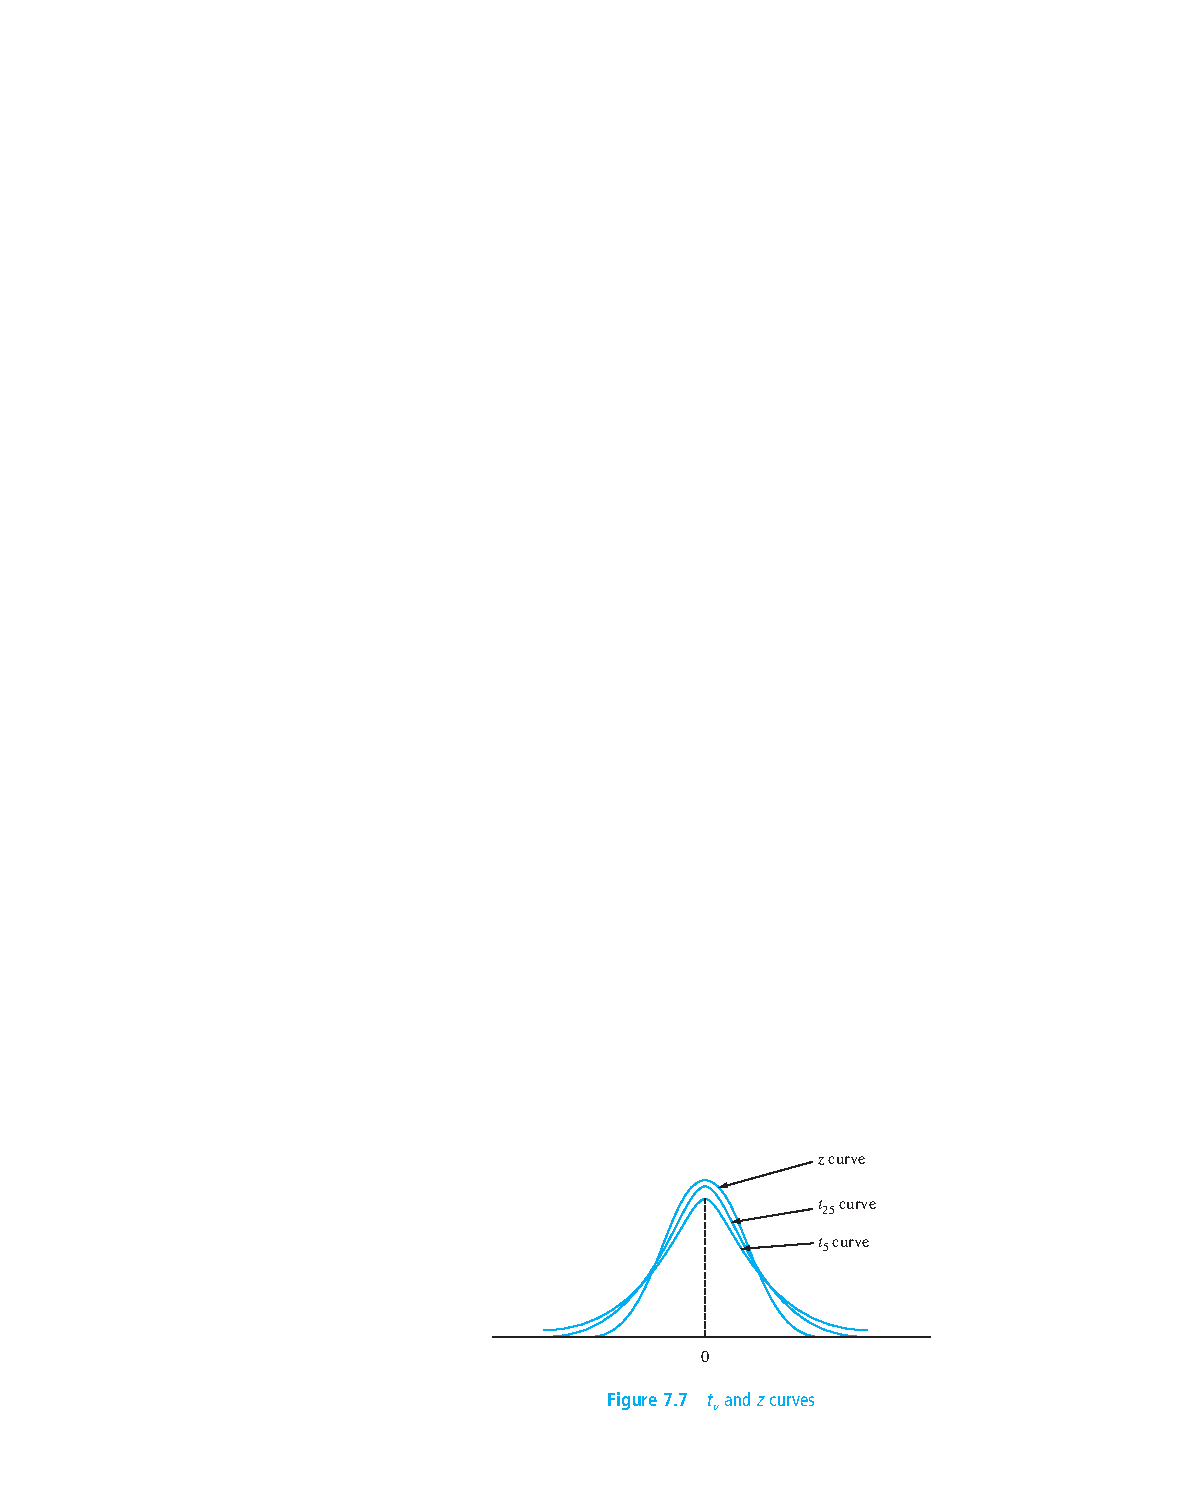
\includegraphics{t_distribution.pdf}
\caption{$t$ and $Z$ distribution}
\end{figure}
\[P\left(-t_{\alpha/2,n-1} \leq \frac{\bar{X}-\mu}{S/\sqrt{n}}  \leq  t_{\alpha/2,n-1} \right) = 1-\alpha\]
where $t_{\alpha/2,n-1}$ denotes the $\frac{\alpha}{2}$-th upper percentile of $t(n-1)$.

Then $\bar{x} \pm  t_{\alpha/2,n-1} \frac{S}{\sqrt{n}} $ is the $100(1-\alpha)\%$ CI for $\mu$.
\end{theo}

\begin{exmp}
The following data are believed to be sampled from normal distribution. 10490, 16620, \dots, 14760 $(n=16)$

Then the 95\% CI for $\mu$ is 

\begin{align*}
\bar{x} \pm  t_{\alpha/2,n-1} \frac{S}{\sqrt{n}}=&14532.5 \pm  t_{0.025,15} \frac{2055.67}{\sqrt{16}}\\
=&(13437.3, 15627.7)
\end{align*} 

\end{exmp}
\subsection{A Prediction Interval for a Single Future Value}
See the corresponding text in the textbook.
\subsection{Tolerance Intervals}
See the corresponding text in the textbook.

% Section 7.3
\section{Large-Sample Confidence Intervals for a Population Mean and Proportion}
\subsection{A Large-Sample Interval for $\mu$}
\begin{prop}
$X_1,\dots,X_n \overset{iid}{\sim} (\mu,\sigma^2)$. $\mu$ and $\sigma$ are both unknown. By CLT if $n$ is large
\[\frac{\bar{X}-\mu}{S/\sqrt{n}} \overset{\cdot}{\sim} N(0,1)\]
\[P\left(-z_{\alpha/2} \leq \frac{\bar{X}-\mu}{S/\sqrt{n}}  \leq  z_{\alpha/2} \right) \overset{\cdot}{=} 1-\alpha\]

Then $100(1-\alpha)\%$ CI for $\mu$ is $\bar{x} \pm  z_{\alpha/2} \frac{s}{\sqrt{n}}$.
\end{prop}

\begin{exmp}
A random sample with $n=48$ is as follows 62, 50, 53,\dots, 50, 56, 58 with $n=48$, $\bar{x}=54.7$, $s=5.23$.

Then the 95\% CI for $\mu$ is 
\[54.7 \pm  z_{0.025} \frac{5.23}{\sqrt{48}}=(53.2, 56.2)\]
\end{exmp}

\subsection{How to Construct a Confidence Interval In General}
$X_1,\dots,X_n \overset{iid}{\sim} f(x;\theta)$. Want to construct a confidence interval for $\theta$
\begin{enumerate}
\item Find a statistic (pivot) which depends on $X_1,\dots,X_n $ and $\theta$ only;
\item Its distribution does not depend on $\theta$ or any other unknown parameters.
\end{enumerate}

\subsection{A General Large-Sample Confidence Interval}
$X_1,\dots,X_n \overset{iid}{\sim} f(x;\theta)$ and $\hat{\theta}$ is an estimate.
For $\theta$, satisfying 
\begin{enumerate}
\item approximately normal 
\item is approxiamtely unbiasd
\item $\sigma_{\hat{\theta}}^2=Var(\hat{\theta})$ is available
\end{enumerate}

Then
\[P\left(-z_{\alpha/2} \leq \frac{\hat{\theta}-\theta}{\sigma_{\hat{\theta}}}  \leq  z_{\alpha/2} \right) = 1-\alpha\]

\subsection{A Confidence Interval for a Population Proportion}
\begin{exmp}
A random sample of $n$ individual is selected from $Bern(p)$. $p=$ success rate.
\[X_1,\dots,X_n \overset{iid}{\sim} Bern(p)\]
\[\boxed{Var(X_i)=p(1-p)  \qquad \hat{p}=\bar{X}}\]
\[Y=\sum_{i=1}^n X_i \sim Bin(n,p)\]

$\hat{p}=\frac{Y}{n}$ is an estimate for $p$. By CLT,
\[\frac{\sqrt{n}(\hat{p}-p)}{\sqrt{p(1-p)}} \overset{\cdot}{\sim} N(0,1)\]
\[P\left(-z_{\alpha/2} \leq \frac{\sqrt{n}(\hat{p}-p)}{\sqrt{p(1-p)}}  \leq  z_{\alpha/2} \right) \overset{\cdot}{=} 1-\alpha\]

So, $100(1-\alpha)\%$ CI for $p$ is $\hat{p} \pm  z_{\frac{\alpha}{2}} \sqrt{\frac{p(1-p)}{n}}$, but $p$ is unknown.
\end{exmp}

\textbf{Remedy}
\begin{enumerate}
\item If $n$ is large, replace $p$ by $\hat{p}$ in the CI formula
$\hat{p} \pm  z_{\frac{\alpha}{2}} \sqrt{\frac{\hat{p}(1-\hat{p})}{n}}$
\item 
\[P\left(-z_{\alpha/2} \leq \frac{\sqrt{n}(\hat{p}-p)}{\sqrt{p(1-p)}}  \leq  z_{\alpha/2} \right) \overset{\cdot}{=} 1-\alpha\]
\[p-z_{\alpha/2}\sqrt{\frac{p(1-p)}{n}} \leq\hat{p}\leq p+z_{\alpha/2}\sqrt{\frac{p(1-p)}{n}} \]
\[(p-\hat{p})^2 \leq z_{\alpha/2}^2 \frac{p(1-p)}{n} \]

Solving the quadratic equation for $p$.
\[\frac{\hat{p}+\frac{z_{\alpha/2}}{2n} \pm z_{\alpha/2}\sqrt{\frac{\hat{p}(1-\hat{p})}{n}+\frac{z_{\alpha/2}^2}{4n^2}}}{1+z_{\alpha/2}^2 /n}\]

is the $100(1-\alpha)\%$ CI for $p$.
\end{enumerate}

\subsection{One-Sided Confidence Intervals (Confidence Bounds)}
\[X_1,\dots,X_n \overset{iid}{\sim} N(\mu,\sigma_0^2)\]
\[P\left(\frac{\bar{X}-\mu}{\sigma_0/\sqrt{n}} \leq z_{\alpha}\right)=1-\alpha\]
Then $P\left(\mu\leq \bar{X}+z_{\alpha}\frac{\sigma_0}{\sqrt{n}}\right)=1-\alpha$. So $\bar{X}+z_{\alpha}\frac{\sigma_0}{\sqrt{n}}$ is the $100(1-\alpha)\%$ upper confidence bound for $\mu$. Similarly, $\bar{X}-z_{\alpha}\frac{\sigma_0}{\sqrt{n}}$ is the $100(1-\alpha)\%$ lower confidence bound for $\mu$. $P\left(\mu\geq \bar{X}-z_{\alpha}\frac{\sigma_0}{\sqrt{n}}\right)=1-\alpha$.

If $\sigma$ is unknown, $\bar{X}+t_{\alpha,n-1}\frac{\sigma_0}{\sqrt{n}}$ is the $100(1-\alpha)\%$ upper confidence bound for $\mu$. $\bar{X}-t_{\alpha,n-1}\frac{\sigma_0}{\sqrt{n}}$ is the $100(1-\alpha)\%$ lower confidence bound for $\mu$.

If large sample, $\bar{x}+z_{\alpha}\frac{s}{\sqrt{n}}$, $\bar{x}-z_{\alpha}\frac{s}{\sqrt{n}}$.

\begin{exmp}
(Example 7.10 in the textbook)
\end{exmp}

\begin{exmp}
37 helmets are tested. 24 of them shown damage: let $p$ denote the proportions of all helmets showing damage under the same impact condition.
\begin{enumerate}
\item Caculate 99\% CI for $p$.
\item What sample size is required for the width of 99\% CI to be at most 0.1?
\end{enumerate}
\textbf{Solution.}

(1) $X=\text{\# of helmets with damages}\sim Bin(37,p)$.
Observe $x=24$, $\hat{p}=\frac{x}{n}=\frac{24}{37}$.

MM: $E(X)=np$, then $n\hat{p}=X$, $\hat{p}=\frac{X}{n}$

MLE: $L(p)= \binom {37}{x} p^x (1-p)^{37-x}$
\[l(p)=\log{\binom {37}{x}}+x \log{p}+(37-x)\log{(1-p)}\]
\[l'(p)=0 \qquad \hat{p}=\frac{x}{n}=\frac{24}{37}\]
\[\hat{p}=\frac{X}{n}\overset{\cdot}{\sim} N\left(p,\frac{p(1-p)}{n}\right)\]
99\% CI for $p$ is $\hat{p} \pm  z_{0.005} \sqrt{\frac{\hat{p}(1-\hat{p})}{n} }=(0.4465,0.8507)$.

(2) Width of 99\% CI is 
\[2 z_{0.005} \sqrt{\frac{\hat{p}(1-\hat{p})}{n} } \leq 0.1\]
\[n \geq \left(\frac{2\times 2.575}{0.1}\right)^2 \hat{p}(1-\hat{p})\]
\[n\geq \left(\frac{2\times 2.575}{0.1}\right)^2 \cdot\frac{1}{4}\]
\end{exmp}

% Section 7.4
\section{Confidence Intervals for the Variance and Standard Deviation of a Normal Population}
\begin{theo}
Then $X_1,\dots,X_n$ are a random sample from $N(\mu,\sigma^2)$. Then
\[\frac{(n-1)S^2}{\sigma^2} \sim \chi^2(n-1)\]
\end{theo}

Then
\[P\left(\chi^2_{1-\alpha/2,n-1} \leq \frac{(n-1)S^2}{\sigma^2} \leq \chi^2_{\alpha/2,n-1} \right)=1-\alpha\]

So $100(1-\alpha)\%$ CI for $\sigma^2$ is
\[\left(\frac{(n-1)s^2}{\chi^2_{\alpha/2,n-1}}, \frac{(n-1)s^2}{\chi^2_{1-\alpha/2,n-1}} \right)\]

Then $100(1-\alpha)\%$ CI for $\sigma$ is
\[\left(	\sqrt{\frac{(n-1)s^2}{\chi^2_{\alpha/2,n-1}}}, \sqrt{\frac{(n-1)s^2}{\chi^2_{1-\alpha/2,n-1}}}\right)\]


\begin{exmp}
(Example 7.15 in the textbook)
\end{exmp}
% chapter 8 
% Last edit: 2017-4-23
\chapter{Tests of Hypotheses Based on a Single Sample}
\section{Hypotheses and Test Procedures}
A test hypothesis is a method using sample data to describe between two competing claims about a population a population characteristic.

\begin{exmp}
$X_1,\dots,X_n \overset{iid}{\sim} f(x;\theta)$

Claim 1: $\theta=0$

Claim 2: $\theta\neq 0$
\end{exmp}

\begin{defn}
Null hypothesis ($H_0$): a population characteristic is usually assumed to be true. Alternative hypothesis ($H_a$): competing claim.

$H_0$ be rejected in favour of $H_a$, if sample evidence suggests that $H_0$ is false.
\end{defn}

\begin{exmp}
\[H_0:\mu=0.75 \qquad H_a:\mu>0.75\]
Only if the sample data strongly suggests that $\theta$ is something different from 0.75, should $H_0$ be rejected. Otherwise, $H_a$ will be rejected.
\end{exmp}

Usually, $H_0:\theta=\theta_0$
\begin{enumerate}
\item $H_a:\theta > \theta_0$ (One-sided alternative)
\item $H_a:\theta <\theta_0$ (One-sided alternative)
\item $H_a:\theta \neq \theta_0$
\end{enumerate}

\begin{exmp}
\[H_0:\mu=0.75 \qquad H_a:\mu>0.75\]
$x_1=0.01,x_2=0.03,x_3=0.02$. Even though the dataset indicates that$\hat{\mu}$ should be very small, if we have to choose one from $H_0,H_a$, choose $H_0$. "Not reject $H_0$".
\end{exmp}


\subsection{Test Procedures}
A test procedure: a rule, based on sample data, for deciding whether to reject $H_0$.

\begin{exmp}
$X$=\# of defective among 200 randomly selected products.
\[H_0:p=0.1 \qquad H_a:p<0.1\]
Here $p$ is the defective rate.
\[X \sim Bin(200,p)\]
Under $H_0 \Rightarrow E(X)=20$. If $H_0$ is true, we would expect $<$ 20 deflective products.

If $x=19,18,17$, they are not strong enough for us to make a decision.

If $x=1,2,3$, they are very strong.
  
\end{exmp}

\noindent\fbox{%
    \parbox{\textwidth}{%
    \textbf{Test Procedure}:
    \begin{enumerate}
    \item A test statistic: a function of sample data on which the decision is made.
    \item Rejection Region (RR): the set of all the statistic values for which $H_0$ will be rejected.
    \end{enumerate}
	}
}

\subsection{Errors in Hypothesis Testing}
\begin{center}
\begin{tabular}{|l|c|c|}
\hline
 & $H_0$ True & $H_0$ False \\
 \hline
 Reject $H_0$ & Type I Error & \checkmark \\
 \hline
 Not Reject $H_0$ & \checkmark & Type II Error \\
 \hline
\end{tabular}
\end{center}
Denote $\alpha=P$(Type I Error), $\beta=P$(Type II Error).

\begin{exmp}
(See Example 8.1 in textbook)
\end{exmp}

\begin{exmp}
(See Example 8.2 in textbook)

As the $\mu$ become smaller and smaller, the probability of Type II error is getting down.
\end{exmp}


\begin{prop}
Suppose the sample size is fixed, and a test statistic is chosen. Then decreasing the size of RR to obtain a small $\alpha$ result in a larger $\beta$ for any particular parameter consisting with $H_a$.
\end{prop}

\subsection{Level-$\alpha$ Test}
A type I error is usually more serious than a type II error. The approach adhered to by most statistical practitioners is then to specify the largest value of $\alpha$ that can be tolerated and find a rejection region having that value of $\alpha$ rather than anything smaller. This makes $\beta$ as small as possible subject to the bound on $\alpha$. The resulting value of $\alpha$ is often referred to as the \textbf{significance level} of the test. Traditional levels of significance are 0.10, 0.05, and 0.01, though the level in any particular problem will depend on the seriousness of a type I error—the more serious this error, the smaller should be the significance level. The corresponding test procedure is called a \textbf{level $\alpha$ test} (e.g., a level 0.05 test or a level 0.01 test). A test with significance level $\alpha$ is one for which the type I error probability is controlled at the specified level.

\begin{exmp}
(See Example 8.5 in textbook)
\begin{align*}
\beta(1.55)= & P(\bar{X}\leq 1.56 \text{ if }H_0 \text{ is false } ) \\
= & P(\bar{X} \leq 1.56) \qquad \bar{X}\sim N\left(1.55,\frac{0.2^2}{32}\right) \\
= & P\left(\frac{\bar{X}-1.55}{\frac{0.2}{\sqrt{32}}} \leq  \frac{1.56-1.55}{\frac{0.2}{\sqrt{32}}} \right)=0.6103
\end{align*}
\end{exmp}



\section{Tests About a Population Mean}
\subsection{Case I: A Normal Population with Known $\sigma_0^2$}
\[H_0:\mu=\mu_0\]
Test statistic \[Z=\frac{\bar{X}-\mu_0}{\sigma_0/\sqrt{n}}\]

Use of the following sequence of steps is recommended when testing hypotheses
about a parameter.
\begin{enumerate}
\item With $H_a: \mu>\mu_0$, $RR:Z\geq c$.

Level-$\alpha$ test
\[P(Z\geq c)\leq 0.05 \Rightarrow x \geq z_{0.05}=1.645 \Rightarrow c=1.645\]
\item With $H_a: \mu<\mu_0$, $RR:Z\leq c$.

Level-$\alpha$ test
\[P(Z\leq c)\leq 0.05 \Rightarrow x \leq -z_{0.05}=-1.645 \Rightarrow c=-1.645\]
\item With $H_a: \mu\neq\mu_0$, $RR:Z\geq c$ or $Z \leq -c$.

Level-$\alpha$ test
\[P(Z\geq c \text{ or } Z \leq -c)\leq 0.05 \Rightarrow x \geq z_{0.025}=1.96 \Rightarrow c=1.96\]
\end{enumerate}


\noindent\fbox{%
    \parbox{\textwidth}{%
\textbf{Conclusion}:

$H_0:\mu=\mu_0$. Test statistic $Z=\frac{\bar{X}-\mu_0}{\sigma_0/\sqrt{n}}$

\begin{enumerate}
\item $H_a:\mu < \mu_0$, $RR: Z\leq -z_{\alpha}$
\item $H_a:\mu > \mu_0$, $RR: Z\geq z_{\alpha}$
\item $H_a:\mu \neq \mu_0$, $RR: |Z|\geq z_{\alpha/2}$ 
\end{enumerate}
	}
}

\subsubsection{Procedure}
\begin{enumerate}
\item identify the parameter of interest
\item determine the null value \& state $H_0$
\item state the "appropriate" $H_a$
\item construct a test statistic
\item for the given significance level $\alpha$, state $RR$
\item compare the observed test statistic' value
\item decide whether to reject $H_0$, give conclusion
\end{enumerate}


\begin{exmp}
(See Example 8.6 in textbook)
\end{exmp}

\subsubsection{$\beta$ and Sample Size Determination}
$H_0:\mu=\mu_0$. 
\[H_a:\mu >\mu_0\]
\[Z=\frac{\bar{X}-\mu_0}{\sigma_0/\sqrt{n}}\overset{H_0}{\sim} N(0,1) \qquad RR: Z\geq z_{\alpha}\]
For $\mu'>\mu_0$: 
\begin{align*}
\beta(\mu')= & P(Z\leq z_{\alpha}) \qquad \bar{X}\sim \left(\mu',\frac{\sigma_0^2}{n}\right) \\
= & P\left(\bar{X}\leq \mu_0+z_{\alpha}\frac{\sigma_0}{\sqrt{n}}\right) \\
= & P\left( \frac{\bar{X}-\mu'}{\sigma_0/\sqrt{n}} \leq \frac{\mu_0+z_{\alpha} \frac{\sigma_0}{\sqrt{n}}-\mu'}	{\sigma_0/\sqrt{n} } \right) \\
= & \Phi\left( \frac{\mu_0-\mu'}	{\sigma_0/\sqrt{n} }++z_{\alpha}  \right)
\end{align*}
Recall that $\Phi$ increases.

$\beta(\mu')$ decreases if $\mu'$ increases, $n$ increases.

If $\beta(\mu')\leq \beta$, $\beta$ is given
\[ \Phi\left( \frac{\mu_0-\mu'}	{\sigma_0/\sqrt{n} }++z_{\alpha}  \right)\leq \beta\]
\[n \geq \left(\frac{z_{\alpha}+ z_{\beta}}{\mu_0-\mu'}\cdot\sigma_0\right)^2\]

For two-sided $H_a$:
\[n \geq \left(\frac{z_{\alpha/2}+ z_{\beta}}{\mu_0-\mu'}\cdot\sigma_0\right)^2\]

\begin{exmp}
(See Example 8.7 in textbook)
\end{exmp}

\subsection{Case II: Large-Sample Tests}
$X_1,\dots,X_n \overset{iid}{\sim} (\mu,\sigma^2)$ with large $n$ ($n \geq 30$)

$H_0:\mu=\mu_0$, $Z=\frac{\bar{X}-\mu_0}{S/\sqrt{n}} \overset{\cdot}{\sim}N(0,1)$
\begin{enumerate}
\item With $H_a: \mu>\mu_0$, $RR:Z\geq z_{\alpha}$.
\item With $H_a: \mu<\mu_0$, $RR:Z\leq -z_{\alpha}$.
\item With $H_a: \mu\neq\mu_0$, $RR:|Z|\geq z_{\alpha/2}$.
\end{enumerate}

\begin{exmp}
(See Example 8.8 in textbook)
\end{exmp}

\subsubsection{$\beta$ and Sample Size Determination}

Determination of $\beta$ and the necessary sample size for these large-sample tests can be based either on specifying a plausible value of $\sigma$ and using the case I formulas (even though $s$ is used in the test) or on using the methodology to be introduced shortly in connection with case III.

\subsection{Case III: A Normal Population Distribution}
\[X_1,\dots,X_n \overset{iid}{\sim} N(\mu,\sigma^2)\]

$H_0:\mu=\mu_0$. Test statistic: $T=\frac{\bar{X}-\mu_0}{S/\sqrt{n}} \sim t(n-1) \text{ under } H_0$

$H_a: \mu>\mu_0$, $RR:\{T\geq ?\}$
\[\alpha=P(\text{Type I Error})=P(T\geq ?) \text{ if }H_0\text{ is true} =P(T\geq t_{\alpha,n-1}) \]

\begin{enumerate}
\item With $H_a: \mu>\mu_0$, $RR:T\geq t_{\alpha,n-1}$.
\item With $H_a: \mu<\mu_0$, $RR:T\leq -t_{\alpha,n-1}$.
\item With $H_a: \mu\neq\mu_0$, $RR:|T|\geq t_{\alpha/2,n-1}$.
\end{enumerate}

\begin{exmp}
$N(\mu,\sigma^2)$, $\sigma$ unknown. Sample: 25.8, 36.6, 26.3, 21.8, 27.2.
\[H_0:\mu=25, \qquad H_a:\mu>25 \]
\[T=\frac{\bar{X}}{S/\sqrt{n}} \sim t(4) \text{ under } H_0\]
\[RR:T\geq t_{0.05,4}=2.132\]
obviously that statistic $T^*=\frac{27.54-25}{5.47/\sqrt{5}}=1.04$. $T^* \notin RR$. Fail to reject $H_0$.
\end{exmp}

\subsubsection{$\beta$ and Sample Size Determination}
See the text in textbook.
\\

\noindent\fbox{%
    \parbox{\textwidth}{%
Claim: 99.9\% of MTR train will be on-time. 
\[X_1,\dots,X_n \overset{iid}{\sim} Bern(p)\]
\[H_0:p=0.999\]
\begin{enumerate}
\item $H_a:p\neq0.999$
\item $H_a:p<0.999$ work against MTR
\item $H_a:p>0.999$ work for MTR
\end{enumerate}
	}
}

\begin{exmp}
(See Exercise 8.32 in textbook)
\end{exmp}

\subsection{Connection to Confidence Interval}
\[X_1,\dots,X_n \overset{iid}{\sim} N(\mu,\sigma_0^2)\]
$\sigma_0$ known. $100(1-\alpha)\%$ CI for $\mu$ is $\bar{x} \pm  z_{\alpha/2} \frac{\sigma_0}{\sqrt{n}} $.
\[H_0:\mu=\mu_0 \qquad H_a:\mu\neq\mu_0\]
\begin{align*}
RR:\left| \frac{\bar{X}-\mu_0}{\sigma_0/\sqrt{n}}\geq z_{\alpha/2} \right| \Leftrightarrow & \mu_0\geq \bar{X}+ z_{\alpha/2} \frac{\sigma_0}{\sqrt{n}} \text{ or } \mu_0\leq \bar{X}- z_{\alpha/2} \frac{\sigma_0}{\sqrt{n}} \\
\Leftrightarrow & \mu_0 \notin \left(\bar{X}-  z_{\alpha/2} \frac{\sigma_0}{\sqrt{n}},\bar{X}+ z_{\alpha/2} \frac{\sigma_0}{\sqrt{n}}\right) \\
\Leftrightarrow & \mu_0 \notin 100(1-\alpha)\% \text{ CI for} \mu
\end{align*}
However, when $H_a$ is not two-sided.
\[ H_a:\mu>\mu_0\]
\begin{align*}
RR: \frac{\bar{X}-\mu_0}{\sigma_0/\sqrt{n}}\geq z_{\alpha} \Leftrightarrow &  \mu_0\leq \bar{X}- z_{\alpha} \frac{\sigma_0}{\sqrt{n}} \\
\Leftrightarrow &  \mu_0 \notin \left(\bar{X}- z_{\alpha} \frac{\sigma_0}{\sqrt{n}},+\infty \right) \\
\Rightarrow & \text{is not a CI for }\mu_0 
\end{align*}

\section{Tests Concerning a Population Proportion}
\subsection{Large-Sample Tests}

Generally, for a parameter $\theta$, if
\begin{enumerate}
\item sample size is large
\item $\hat{\theta}$ is approximately normal
\item $\sigma_{\hat{\theta}}^2$ is available
\end{enumerate}

Test statistic: $Z=\frac{\hat{\theta}-\theta}{\sigma_{\hat{\theta}}}$.

Suppose $X\sim Bin(n,p)$, $\hat{p}=\frac{X}{n}$, $Var(\hat{p})=Var\left(\frac{X}{n}\right)=\frac{p(1-p)}{n}$
\[Z=\frac{\hat{p}-p}{\sqrt{\frac{p(1-p)}{n}}} \overset{\cdot}{\sim}N(0,1)\]
\[H_0:p=p_0 \qquad H_a:p>p_0\]
\[Z=\frac{\hat{p}-p_0}{\sqrt{\frac{p_0(1-p_0)}{n}}} \overset{\cdot}{\sim}N(0,1) \text{ under }H_0\]

Reject $H_0$ if $Z\geq z_{\alpha}$.

\begin{exmp}
(See Exercise 8.39 in textbook)
A random sample of 150 recent donations at a certain blood bank reveals that 82 were type A blood. Does this suggest that the actual percentage of type A donations differs from 40\%, the percentage of the population having type A blood? Carry out a test of the appropriate hypotheses using a significance level of 0.01. Would your conclusion have been different if a significance level of 0.05 had been used?
\end{exmp}


\subsubsection{$\beta$ and Sample Size Determination}
\[H_0:p=p_0 \qquad H_a:p'>p_0\]
\[RR:Z=\frac{\frac{X}{n}-p_0}{\sqrt{\frac{p_0(1-p_0)}{n}}}\geq z_{\alpha}\]
\begin{align*}
\beta(p') =& P(\text{fail to reject }H_0 \text{ if }H_0 \text{ is false}) \\
= & P(Z\leq z_{\alpha}) \qquad X \sim Bin(n,p') \\
= & P\left(\frac{\frac{X}{n}-p_0}{\sqrt{\frac{p_0(1-p_0)}{n}}} \leq z_{\alpha}\right) = P\left(\frac{X}{n}\leq p_0+z_{\alpha}\sqrt{\frac{p_0(1-p_0)}{n}} \right) \\
= & P\left( \frac{\frac{X}{n}-p'}{\sqrt{\frac{p'(1-p')}{n}}}  \leq \frac{p_0+z_{\alpha}\sqrt{\frac{p_0(1-p_0)}{n}}-p'}{\sqrt{\frac{p'(1-p')}{n}}} \right) \\
= & \Phi\left(\frac{p_0+z_{\alpha}\sqrt{\frac{p_0(1-p_0)}{n}}-p'}{\sqrt{\frac{p'(1-p')}{n}}}\right) \leq \beta
\end{align*}
\[\frac{p_0+z_{\alpha}\sqrt{\frac{p_0(1-p_0)}{n}}-p'}{\sqrt{\frac{p'(1-p')}{n}}} \leq -z_{\beta} \Rightarrow n \geq \left( \frac{z_{\alpha}\sqrt{p_0(1-p_0)}+z_{\beta}\sqrt{p'(1-p')}}{p'-p_0}\right)^2\]

"One-sided" for $p'<p_0$
\[\beta(p')= 1- \Phi\left(\frac{p_0-p'-z_{\alpha}\sqrt{\frac{p_0(1-p_0)}{n}}}{\sqrt{\frac{p'(1-p')}{n}}}\right) \leq \beta \]

"Two-sided" for $p'\neq p_0$
\[\beta(p')= \Phi\left(\frac{p_0-p'+z_{\alpha/2}\sqrt{\frac{p_0(1-p_0)}{n}}}{\sqrt{\frac{p'(1-p')}{n}}}\right)- \Phi\left(\frac{p_0-p'-z_{\alpha/2}\sqrt{\frac{p_0(1-p_0)}{n}}}{\sqrt{\frac{p'(1-p')}{n}}}\right) \leq \beta \]

\begin{exmp}
(See Example 8.12 in textbook)
\end{exmp}

\subsection{Small-Sample Tests}
\[H_0:p=p_0 \qquad H_a:p>p_0\]
Observe $X \sim Bin(n,p)$, reject $H_0$ if $X\geq c$.
\begin{align*}
P(\text{Type I error})= & P(X \geq x) \qquad \text{ if }H_0 \text{ is true} \\
= & 1- B(c-1;n;p_0) \leq\alpha
\end{align*}
\begin{align*}
\beta(p')= & P(X \leq c-1) \qquad X \sim Bin(n,p') \\
= & B(c-1;n;p')
\end{align*}

\begin{exmp}
(See Example 8.13 in textbook)
\end{exmp}

\section{$P$-Values}
\begin{exmp}
In a community, the mean household water usage for Jan. 93 is 0.6. In 94, water conservation was conducted. In Jan. 95, $n=50$ households are randomly selected. $n=50,\bar{x}=0.054,s=0.016$. Does the data suggest that the water usage become less?
\[H_0:\mu=0.6 \qquad H_a:\mu<0.6\]
\[Z=\frac{\bar{X}-0.6}{S/\sqrt{n}}\overset{H_0}{\sim} N(0,1)\]
\[RR: Z\leq z_{-\alpha}=\begin{cases}
-1.645 &\text{if }\alpha=0.05, \\
-2.33 &\text{if }\alpha=0.01, 
\end{cases}\]
\[z^*=\frac{0.054-0.6}{0.016/\sqrt{50}}=-2.61\]

If $\alpha=0.05$, reject $H_0$; If $\alpha=0.01$, reject $H_0$.

$P$-value: $P(Z\leq-2.61)=0.0045$. Consider $\alpha=0.0045$, $RR:Z\leq-2.61$.
\end{exmp}

\begin{defn}
$P$-value is the smallest level of significance at which $H_0$ will be rejected when the test is used on a given database.
\end{defn}

\noindent\fbox{%
    \parbox{\textwidth}{%
Conclusion:

If $P$-value$\leq \alpha$, then reject $H_0$. If $P$-value$\geq \alpha$, then fail to reject $H_0$. 
	}
}

\begin{defn}
The P-value is the probability, calculated assuming that the null hypothesis is true, of obtaining a value of the test statistic at least as contradictory to $H_0$ as the value calculated from the available sample. The smaller the $P$-value, the more contradiction is the data to $H_0$.
\end{defn}

\subsection{$P$-Values for z Tests}
\subsubsection{Case I: A Normal Population with Known $\sigma_0^2$}
\[X_1,\dots,X_n \overset{iid}{\sim} N(\mu,\sigma_0^2)\]

$H_0:\mu=\mu_0$. Test statistic $Z=\frac{\bar{X}-\mu_0}{\sigma_0/\sqrt{n}}$

$H_a:\mu>\mu_0$. $P$-value $= P(Z \geq Z^*)$

$H_a:\mu<\mu_0$. $P$-value $= P(Z \leq Z^*)$

$H_a:\mu\neq\mu_0$. $P$-value $= P(|Z| \geq |Z^*|)=2(1-\Phi(|Z^*|))$

\subsubsection{Case II: Large-Sample Tests}
Similar as Case I.

\begin{exmp}
(See Example 8.17 in textbook)
\end{exmp}

\subsection{$P$-Values for t Tests}
\[X_1,\dots,X_n \overset{iid}{\sim} N(\mu,\sigma^2)\]

$H_0:\mu=\mu_0$. Test statistic: $T=\frac{\bar{X}-\mu_0}{S/\sqrt{n}} \sim t(n-1) \text{ under } H_0$

$H_a:\mu>\mu_0$. $P$-value $= P(T \geq T^*)=1-CDF_{n-1}(T^*)$

$H_a:\mu<\mu_0$. $P$-value $= P(T \leq T^*)=CDF_{n-1}(T^*)$

$H_a:\mu\neq\mu_0$. $P$-value $= P(|T| \geq |T^*|)=2(1-CDF_{n-1}(|T^*|))$

\begin{exmp}
Six readings from a device: 85, 77, 82, 68, 72, 69. It is believed that the CO concentration is set at 70 ppm. Is recalibration of this device necessary? $\alpha=0.05$

$H_0:\mu=70$. Test statistic: $T=\frac{\bar{X}-70}{S/\sqrt{n}} \overset{H_0}{\sim} t(n-1) $

$H_a:\mu\neq 70$. $T^*=\frac{75.5-70}{7/\sqrt{6}}=1.92 $
\[P-Value=P(|T|\geq 1.92)=2(1-CDF_5(1.92))=0.116>0.05\]

Fail to reject $H_0$.
\end{exmp}

\section{Hypotheses Testing For $\sigma^2$}
Then $X_1,\dots,X_n$ are a random sample from $N(\mu,\sigma^2)$. $\mu,\sigma^2$ unknown.

(a)\[H_0:\sigma^2=\sigma_0^2 \qquad H_a:\sigma^2 \neq\sigma_0^2\]
\[\frac{(n-1)S^2}{\sigma^2} \overset{H_0}{\sim} \chi^2(n-1)\]
\[RR:\{\chi^2 \leq \chi^2_{1-\alpha/2,n-1} \text{ or } \chi^2 \geq \chi^2_{\alpha/2,n-1}\}\]

(b) $H_a:\sigma^2 >\sigma_0^2$, $RR:\{\chi^2 \geq \chi^2_{\alpha,n-1}\}$

(c) $H_a:\sigma^2 <\sigma_0^2$, $RR:\{\chi^2 \leq \chi^2_{1-\alpha,n-1}\}$

\begin{exmp}
A battery manufacture claims that he produce batteries have a s.d. equal to 0.9 year. A random sample is collected $n=10$, $s=1.2$ year. Does the data suggest that $\sigma>0.9$? Assume normality.

\[H_0:\sigma=0.9 \qquad H_a:\sigma \geq 0.9\]
\[H_0:\sigma^2=0.81 \qquad H_a:\sigma^2 \geq 0.81\]
\[\frac{(n-1)S^2}{0.81} \overset{H_0}{\sim} \chi^2(n-1)\]
$RR:\{\chi^2 \geq \chi^2_{0.05,9}\}=\{\chi^2 \geq 16.919\}$
\[(\chi^2)^*=\frac{(10-1)1.2^2}{0.9^2}=16.0 \notin RR \]
Fail to reject $H_0$.
\[P-Value=P(\chi^2\geq (\chi^2)^* )=P(\chi^2\geq  16)=0.07\]
$P$-Value $>0.05$, fail to reject $H_0$.
\end{exmp}
% chapter 9
% Last edit: 2017-4-24
\chapter{Inferences Based on Two Samples}
\section{z Tests and Confidence Intervals for a Difference Between Two Population Means}

$X_1,\dots,X_n \overset{iid}{\sim} N(\mu_1,\sigma_1^2)$, $\sigma_1$ known.

$Y_1,\dots,Y_n \overset{iid}{\sim} N(\mu_2,\sigma_2^2)$, $\sigma_2$ known.

\begin{prop}
\[E(\bar{X}-\bar{Y})=\mu_1-\mu_2\]
\[Var(\bar{X}-\bar{Y})=\frac{\sigma_1^2}{n}+\frac{\sigma_2^2}{n}\]
\end{prop}

\subsection{Test Procedures for Normal Populations with Known Variances}
Case I
\[Z=\frac{\bar{X}-\bar{Y}-(\mu_1-\mu_2)}{\sqrt{\frac{\sigma_1^2}{n}+\frac{\sigma_2^2}{n}}} \sim N(0,1)\]

$H_0:\mu_1-\mu_2=\Delta_0$
\begin{enumerate}
\item With $H_a: \mu_1-\mu_2>\Delta_0$, $RR:Z\geq z_{\alpha}$.
\item With $H_a: \mu_1-\mu_2<\Delta_0$, $RR:Z\leq -z_{\alpha}$.
\item With $H_a: \mu_1-\mu_2\neq\Delta_0$, $RR:|Z|\geq z_{\alpha/2}$.
\end{enumerate}

\begin{exmp}
(See Example 9.1 in textbook)
\end{exmp}

\subsection{Large-Sample Tests}
Case II large sample, $\sigma^2$ unknown

\[Z=\frac{\bar{X}-\bar{Y}-(\mu_1-\mu_2)}{\sqrt{\frac{S_1^2}{n}+\frac{S_2^2}{n}}} \sim N(0,1)\]

$100(1-\alpha)$ CI for $\mu_1-\mu_2$
\[ \bar{X}-\bar{Y} \pm z_{\alpha/2} \sqrt{\frac{S_1^2}{n}+\frac{S_2^2}{n}} \]

\section{The Two-Sample t Test and Confidence Interval}
Case III

(a) $X_1,\dots,X_n \overset{iid}{\sim} N(\mu_1,\sigma_1^2)$

$Y_1,\dots,Y_n \overset{iid}{\sim} N(\mu_2,\sigma_2^2)$. $\sigma_1$,$\sigma_2$ independent 

\[T=\frac{\bar{X}-\bar{Y}-(\mu_1-\mu_2)}{\sqrt{\frac{S_1^2}{n}+\frac{S_2^2}{n}}} \sim t(\nu) \qquad \nu=\frac{\left( \frac{S_1^2}{n}+\frac{S_2^2}{n} \right)^2}{ \frac{\left( \frac{S_1^2}{m} \right)^2}{m-1}+ \frac{\left( \frac{S_1^2}{m} \right)^2}{n-1}  } \]

$100(1-\alpha)$ CI for $\mu_1-\mu_2$
\[\bar{X}-\bar{Y} \pm t_{\alpha/2,\nu} \sqrt{\frac{S_1^2}{n}+\frac{S_2^2}{n}}  \]

\[H_0:\mu_1-\mu_2=\Delta_0 \qquad T=\frac{\bar{X}-\bar{Y}-\Delta_0}{\sqrt{\frac{S_1^2}{n}+\frac{S_2^2}{n}}} \sim t(\nu)\]
\begin{enumerate}
\item With $H_a: \mu_1-\mu_2>\Delta_0$, $RR:T\geq t_{\alpha,nu}$.
\item With $H_a: \mu_1-\mu_2<\Delta_0$, $RR:T\leq -t_{\alpha,nu}$.
\item With $H_a: \mu_1-\mu_2\neq\Delta_0$, $RR:|T|\geq t_{\alpha/2,nu}$.
\end{enumerate}

\begin{exmp}
(See Example 9.6 in textbook)
\end{exmp}

\subsection{Pooled t Procedures}
(b) Small sample size, $\sigma_1^2=\sigma_2^2$

\[T=\frac{\bar{X}-\bar{Y}-(\mu_1-\mu_2)}{\sqrt{\frac{S_p^2}{n}+\frac{S_p^2}{n}}}\]

\[S_p=\frac{n-1}{m+n-2}S_1^2+\frac{m-1}{m+n-2}S_2^2\]

"pooled sample variance"

\[S_1^2=\frac{1}{n-1} \sum_{i=1}^n (X_i-\bar{X})^2 \qquad S_2^2=\frac{1}{m-1} \sum_{i=1}^m (Y_i-\bar{Y})^2 \]

\begin{exmp}
Body weight gained on animal treatment: given 1mg/peller dose of soft steroid control: placebo.

\begin{tabular}{l|c|c|c}
\hline
treatment & $m=8$ & $\bar{x}=32.8$ & $s_1=2.6$ \\
\hline
placebo & $n=8$ & $\bar{y}=40.5$ & $s_2=2.5$ \\
\hline
\end{tabular}

Does the data suggest the average weight gain in the control group exceeds that in the treatment group by more than 5g? $\alpha$

\begin{enumerate}
\item $H_0:\mu_1-\mu_2 = -5 \qquad H_a:\mu_1-\mu_2 < -5$
\[T^*=\frac{\bar{X}-\bar{Y}-(-5)}{\sqrt{\frac{S_1^2}{n}+\frac{S_2^2}{n}}}=-2.23 \]
\[\nu=\frac{\left( \frac{S_1^2}{n}+\frac{S_2^2}{n} \right)^2}{ \frac{\left( \frac{S_1^2}{m} \right)^2}{m-1}+ \frac{\left( \frac{S_1^2}{m} \right)^2}{n-1}  }=\frac{\left(\frac{2.6^2}{8}+\frac{2.5^2}{10}\right)^2}{\frac{1}{7} \left(\frac{2.6^2}{8}\right)^2+\frac{1}{9} \left(\frac{2.5^2}{10}\right)^2}=14.886 \approx 14\]
\[P-Value=P(T_{14}\leq T^*)=0.022>0.1\]
\item Assume $\sigma_1^2=\sigma_2^2$

$H_0:\mu_1-\mu_2 = -5 \qquad H_a:\mu_1-\mu_2 < -5$

\[T^*=\frac{\bar{X}-\bar{Y}-(-5)}{\sqrt{\frac{S_p^2}{n}+\frac{S_p^2}{n}}}=-2.24\]
Here $S_p=\sqrt{\frac{2.6^2 (8-1)}{8+10-2}+\frac{2.5^2 (10-1)}{8+10-2}}=2.54$

\[P-Value=P(T_{16}<-2.24)=0.021>0.01\]

\end{enumerate}
\end{exmp}

\section{Analysis of Paired Data}
$n$ independent selected pairs
$(X_1,Y_1),(X_2,Y_2),\dots,(X_n,Y_n)$

\[E(X_i)=\mu_1 \qquad E(Y_i)=\mu_2\]
\[H_0:\mu_1-\mu_2=\Delta \qquad H_a:\mu_1-\mu_2 \neq\Delta\]
\begin{center}
\begin{tabular}{ccccc}
\hline
$X$ & $X_1$ & $X_2$ & \dots & $X_n$ \\ 
$Y$ & $Y_1$ & $Y_2$ & \dots & $Y_n$ \\ 
$D=X-Y$ & $D_1=X_1-Y_1$ & $D_2=X_2-Y_2$ & \dots & $D_n=X_n-Y_n$ \\
\hline
\end{tabular}
\end{center}

\[H_0:\mu_D=\mu_1-\mu_2=\Delta \qquad H_a:\mu_D=\mu_1-\mu_2 \neq\Delta\]
\[D_1,D_2,\dots,D_n\]

\[T=\frac{\bar{D}-\Delta}{S_D/\sqrt{n}}\]
\[\bar{D}=\frac{1}{n}\sum_{i=1}^n D_i \qquad  S_D^2=\frac{1}{n-1}\sum_{i=1}^n (D_i-\bar{D})^2\]

\subsection{The Paired t Test}

\begin{exmp}
(See Exercise 8.39 in textbook) reports the accompanying data on amount of milk ingested by each of 14 randomly selected infants.

Does it appear that the true average difference between intake values measured by the two methods is something other than zero? Determine the $P$-value of the test, and use it to reach a conclusion at significance level 0.05.


\end{exmp}

$100(1-\alpha)$\% CI for $\mu_1-\mu_2=\mu_0$
\[\bar{D} \pm t_{\alpha/2,n-2}\frac{S_D}{\sqrt{n}}\]

\section{Inferences Concerning a Difference Between Population Proportions}

\begin{prop}
Let $X\sim Bin(n,p_1)$, $Y\sim Bin(m,p_2)$ with $X$ and $Y$ independently. $\hat{p_1}=\frac{X}{n}$,$\hat{p_2}=\frac{Y}{m}$
\[E(\hat{p_1}-\hat{p_2})=p_1-p_2\]
\[Var(\hat{p_1}-\hat{p_2})=\frac{p_1(1-p_1)}{n}+\frac{p_2(1-p_2)}{m}\]
\end{prop}

As $n$ and $m$ get larger,
\[Z=\frac{\hat{p_1}-\hat{p_2}-(p_1-p_2)}{\sqrt{\frac{p_1(1-p_1)}{n}+\frac{p_2(1-p_2)}{m}}} \overset{iid}{\sim} N(0,1)\]

$100(1-\alpha)$\% CI for $p_1-p_2$
\[\hat{p_1}-\hat{p_2} \pm z_{\alpha/2}\sqrt{\frac{\hat{p_1}(1-\hat{p_1})}{n}+\frac{\hat{p_2}(1-\hat{p_2})}{m}}\]

\subsection{A Large-Sample Test Procedure}

To test $H_0$: $p_1-p_2=0$

Test statistic: \[Z=\frac{\hat{p_1}-\hat{p_2}-0}{\sqrt{\hat{p}(1-\hat{p}) \left(\frac{1}{n}+\frac{1}{m} \right)}}\] 

where $\hat{p}=\frac{X+Y}{n+m}$

\begin{enumerate}
\item With $H_a: p_1-p_2>0$, $RR:Z \geq z_{\alpha}$.
\item With $H_a: p_1-p_2<0$, $RR:Z \leq -z_{\alpha}$.
\item With $H_a: p_1-p_2\neq 0$, $RR:|Z|\geq z_{\alpha/2}$.
\end{enumerate}


\begin{exmp}
\begin{tabular}{c|c|c}
\hline
	& plea guilty & plea not guilty \\ \hline
Judged guilty	& $m=191$ & $n=64$ \\ \hline
Sentenced to prison & $x=101$ & $y=56$ \\ \hline
\end{tabular}

\[H_0: p_1-p_2=0 \qquad p_1\neq p_2\]
\[\hat{p_1}=\frac{101}{191}=0.53 \qquad \hat{p_2}=\frac{56}{64}=0.875\]
\[Z=\frac{\hat{p_1}-\hat{p_2}-0}{\sqrt{\hat{p}(1-\hat{p}) \left(\frac{1}{n}+\frac{1}{m} \right)}} \qquad \hat{p}=\frac{101+56}{191+64}=0.616\] 
\[Z^*=-4.91 \qquad RR:\{|Z|\geq z_{\alpha/2}=2.58\} \quad \alpha=0.01\]
\[Z^* \in RR \Rightarrow \text{Reject }H_0\]

Conclusion:
\end{exmp}

\section{Challenge Question 4}
\begin{figure}[H]
\centering
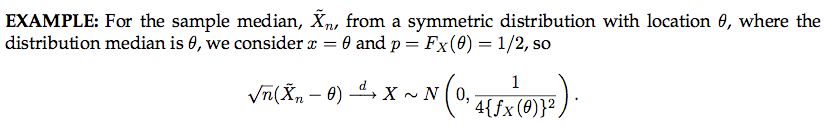
\includegraphics[scale=0.5]{median.jpeg}
\end{figure}

\begin{proof}
\[\lim_{n \to\infty} P(\sqrt{n}(\tilde{X_n}-\theta)\leq a)=P(Z \leq 2 f(\theta)a)\]

Let $Y_i=I\left(X_i\leq \theta+\frac{a}{\sqrt{n}}\right) \qquad i=1,2,\dots,n$
\[Y_i=\begin{cases}
1, & x_i\leq \theta+\frac{a}{\sqrt{n}} \\
0. & x_i\geq \theta+\frac{a}{\sqrt{n}} 
\end{cases}\]

Clearly, $Y_1,Y_2,\dots,Y_n \overset{iid}{\sim} Bern(p_n)$

\[p_n=P\left(X_i\leq \theta+\frac{a}{\sqrt{n}}\right)=F\left( \theta+\frac{a}{\sqrt{n}}\right)\]

\begin{align*}
P(\sqrt{n}(\tilde{X_n}-\theta)\leq a)= & P\left(\tilde{X_n}\leq \theta+\frac{a}{\sqrt{n}}\right)\\
= & P\left( \sum_{i=1}^{n} Y_i \geq \frac{n+1}{2} \right) \\
= & P\left(\frac{\sum_{i=1}^{n} Y_i -n p_n}{\sqrt{n p_n(1-p_n)}} \geq \frac{\frac{n+1}{2} -n p_n}{\sqrt{n p_n(1-p_n)}}\right)
\end{align*}

Note that $p_n \to\frac{1}{2}, n\to \infty$. By CLT,

\[ \frac{\sum_{i=1}^{n} Y_i -n p_n}{\sqrt{n p_n(1-p_n)}}  \overset{d}{\to} N(0,1)\]

\[\lim_{n\to\infty} \frac{F\left(\theta+\frac{a}{\sqrt{n}}-F(\theta)\right)}{a/\sqrt{n}}=F'(\theta)=f(\theta)\]

\[\frac{n\left(p_n-\frac{1}{2}\right)}{\sqrt{n}} \longrightarrow f(\theta)\cdot a\]

\[\frac{np_n-\frac{n+1}{2}}{\sqrt{n}} \longrightarrow f(\theta)\cdot a \qquad \sqrt{p_n(1-p_n)} \longrightarrow \frac{1}{2} \qquad n\to\infty\]

\[\frac{\frac{n+1}{2} -n p_n}{\sqrt{n p_n(1-p_n)}}\longrightarrow -2af(\theta)\]
\end{proof}

Another proof: Bootstrap.
\begin{proof}
$X_1,\dots,X_n \overset{iid}{\sim} f(x)$. Distribution of $\tilde{X_n}$

Bootstrap: if $f(x)$ is "known"
\begin{align*}
\tilde{X_n^{(1)}} \leftarrow & X_1^{(1)} \dots X_n^{(1)} \overset{iid}{\sim} f(x)  \\
\tilde{X_n^{(2)}} \leftarrow & X_1^{(2)} \dots X_n^{(2)} \overset{iid}{\sim} f(x)  \\
\tilde{X_n^{(3)}} \leftarrow & X_1^{(3)} \dots X_n^{(3)} \overset{iid}{\sim} f(x)  \\
\dots\dots & \dots\dots\dots\dots\dots\dots \\
\tilde{X_n^{(B)}} \leftarrow & X_1^{(B)} \dots X_n^{(B)} \overset{iid}{\sim} f(x)  
\end{align*}
\[\tilde{f(x)}=\frac{1}{n} \qquad \text{if } x=x_i\]
Sample $n$ values from $\{x_1,\dots,x_n\}$ with replacement.
\end{proof}
% Appendix
% Last edit: 2017-5-4
\appendix
\chapter{Moment generating function}
\section{Definition}
\begin{defn}
The moment generating function (MGF) of a r.v. $X$ is defined as
\[M_X(\theta)=E(e^{\theta x})=\begin{cases}
\sum_{x \in \mathcal{D}} e^{\theta x} p(x) & \text{if }X \text{ is discrete}	\\
\int_{-\infty}^{\infty} e^{\theta x} f(x)\,dx & \text{if }X \text{ is continues}	
\end{cases} \]
\end{defn}

\begin{exmp}
If $Z \sim N(0,1)$. Find the mgf $M_Z(\theta)$
\begin{align*}
M_Z(\theta)=E(e^{\theta x})=& \int_{-\infty}^{\infty} e^{\theta z} \frac{1}{\sqrt{2 \pi}} e^{-\frac{1}{2} z^2} \, dz \\
= & \int_{-\infty}^{\infty}  \frac{1}{\sqrt{2 \pi}} e^{\theta z-\frac{1}{2} z^2} \,dz\\
= & \int_{-\infty}^{\infty}  \frac{1}{\sqrt{2 \pi}} e^{-\frac{1}{2}\theta^2 + \theta z-\frac{1}{2} z^2 } e^{\frac{1}{2}\theta^2} \,dz\\
= & e^{\frac{1}{2} \theta^2}
\end{align*}
\end{exmp}

\section{Properties of $M_X{\theta}$}
\begin{prop}
\begin{enumerate}
\item There is a unique distribution with mgf $M_X{\theta}$
\item \begin{align*}
M_X{\theta}=& E(e^{\theta x}) \\
=& E\left(1+\frac{\theta X}{1!}+ \frac{\theta^2 X^2}{2!}+\dots \right) \\
=& 1+\frac{\theta E(X)}{1!}+ \frac{\theta^2 E(X)^2}{2!}+\dots
\end{align*}
\item 
\[\frac{d M_X(\theta)}{d \theta}=\frac{d E(e^{\theta x})}{d \theta}=E\left(\frac{d e^{\theta x}}{d \theta}\right)=E(e^{\theta X} X)\]
\[\left.\frac{d M_X(\theta)}{d \theta}\right|_{\theta=0}=E(X)\]

Similarly,
\[\left.\frac{d^r M_X(\theta)}{d \theta^r}\right|_{\theta=0}=E(X^r) \qquad r=1,2,\dots,\]
\item Let $Y=a+bX$, then $M_Y(\theta)=e^{a\theta} M_X(b\theta)$
\[M_Y(\theta)=E(E^{\theta Y})=E(e^{\theta (a+bX)})=E(e^{a\theta+b\theta x})=e^{a\theta} E(e^{b\theta x})=e^{a \theta}M_X(b\theta)\]
\end{enumerate}
\end{prop}

\begin{exmp}
If $X \sim N(\mu,\sigma^2)$, find $M_Y(\theta)$
\[Z=\frac{X-\mu}{\sigma}\sim N(0,1) \text{ then } X=\mu+\sigma Z\]

by (4)
\[M_Y(\theta)=e^{\mu \theta} M_Z(\sigma \theta)=e^{\mu\theta+\frac{1}{2} \sigma^2\theta^2}\]
\[E(Y)=\left.\frac{d M_Y(\theta)}{d \theta}\right|_{\theta=0}=\mu\]
\[E(Y^2)=\left.\frac{d^2 M_Y(\theta)}{d \theta^2}\right|_{\theta=0}=\mu^2+\sigma^2\]
\[E(Y^3)=\left.\frac{d^3 M_Y(\theta)}{d \theta^3}\right|_{\theta=0}=\dots\]
\end{exmp}

\begin{theo}
$X$ and $Y$ are two independent r.v. with mgf $M_X(\theta)$ and $M_Y(\theta)$ respectively. Then 
\[M_{X+Y}(\theta)=M_X(\theta)M_Y(\theta)\]
\begin{proof}
\[M_{X+Y}(\theta)=E(e^{\theta(X+Y)})=E(e^{\theta X} e^{\theta Y})=M_X(\theta)M_Y(\theta)\]
\end{proof}
\end{theo}

\begin{coro}
If $X_1,\dots,X_n$ are independent r.v.'s
\[M_{X_1+\dots+X_n}(\theta)=M_{X_1}(\theta)\dots M_{X_n}(\theta)\]
\end{coro}

\begin{exmp}
\begin{enumerate}
\item $Z^2 \sim \chi^2(1)$
\item $Z_1,\dots,Z_n \overset{iid}{\sim} N(0,1)$, then 
\[Z_1^2 +Z_2^2+\dots+Z_n^2 \sim \chi^2(n)\] 
\end{enumerate}
\begin{proof}
\begin{enumerate}
\item \begin{align*}
M_{Z^2}(\theta)=E(e^{\theta z^2}) = & \int_{-\infty}^\infty e^{\theta z^2} \frac{1}{\sqrt{2 \pi}} e^{-\frac{1}{2} z^2} \, dz \\
= & \int_{-\infty}^\infty \frac{1}{\sqrt{2 \pi}} e^{\left(\theta-\frac{1}{2}\right) z^2} \,dz \\
= & \int_{-\infty}^\infty  \frac{1}{\sqrt{2 \pi}} e^{-\frac{1}{2}\left(-2\theta+1\right) z^2} \,dz \\
= & \int_{-\infty}^\infty  \frac{1}{\sqrt{2 \pi}} e^{-\frac{1}{2} y^2} \frac{1}{\sqrt{1-2\theta}} \,dy \\
= & \frac{1}{\sqrt{1-2\theta}} \qquad \theta<\frac{1}{2}
\end{align*}

Assume $\theta <\frac{1}{2}$, Let $y=\sqrt{1-2\theta} z$.

Let $A \sim \chi^2(1)$, then
\[f_A(x)=\frac{1}{2^{1/2} \Gamma(1/2)} a^{-\frac{1}{2}} e^{-\frac{a}{2}}	\]

Then
\begin{align*}
M_A(\theta)=E(e^{\theta A}) = & \int_0^\infty	e^{\theta a}\frac{1}{2^{1/2} \Gamma(1/2)} a^{-\frac{1}{2}} e^{-\frac{a}{2}}\,da	\\
= & \int_0^\infty \frac{1}{2^{1/2} \Gamma(1/2)}  a^{-\frac{1}{2}} e^{\left(\theta-\frac{1}{2}\right)a}\,da \\
= & \int_0^\infty \frac{1}{\Gamma(1/2)} (1-2\theta)^{\frac{1}{2}} t^{-\frac{1}{2}} e^{-t} \,dt	\\
= & (1-2\theta)^{-\frac{1}{2}}  \qquad \theta<\frac{1}{2}
\end{align*}

Let $t=\frac{1}{2} (1-2\theta)a$, $\theta<\frac{1}{2}$ 

Since $M_{Z^2}(\theta)=M_A(\theta) \Rightarrow Z^2\sim A\sim \chi^2(1)$
\item Let $S=Z_1^2 +Z_2^2+\dots+Z_n^2$
\[M_S(\theta)=(1-2\theta)^{-\frac{n}{2}}\]

Let $B \sim \chi^2(n)$
\[f_B(b)=\frac{1}{2^{n/2} \Gamma(n/2)} b^{\frac{n}{2}-1} e^{-\frac{b}{2}}	\]
\[M_B(\theta)= \int_0^\infty e^{\theta b}	\frac{1}{2^{n/2} \Gamma(n/2)} b^{\frac{n}{2}-1} e^{-\frac{b}{2}} \,b=(1-2\theta)^{-\frac{n}{2}}\]
\[M_S(\theta)=M_B(\theta) \Rightarrow S \sim B \sim \chi^2(n)\]
\end{enumerate}
\end{proof}
\end{exmp}

\section{Application}
\begin{theo}
Let $Y_1,Y_2,\dots,Y_n$ be a sequence of rv's with cdf $F_{Y_1}(y)$, $F_{Y_2}(y)$, \dots and mgf $M_{Y_1}(\theta), M_{Y_2}(\theta),\dots $. Suppose as $n \to\infty$ 

\[M_{Y_n}(\theta) \rightarrow M_Y(\theta) \text{ for any }\theta\]

where $M_Y(\theta)$ is the mgf of $Y$ with cdf $F(y)$ that
\[F_{Y_n} \rightarrow F_Y(y) \text{ for any }y \text{ as }n \to \infty\]

or $Y_n\overset{d}{\longrightarrow} Y$.\footnote{converge to distribution}
\end{theo}

\begin{exmp}
If $X_n\sim Bin(n,p)$. $np=\lambda>0$. fixed
\begin{align*}
M_{X_n}(\theta)= & E(e^{\theta X_n}) =\sum_{i=1}^n e^{\theta k} {n \choose k} p^k (1-p)^{n-k}\\
= & \sum_{k=0}^n {n \choose k} (pe^{\theta})^k (1-p)^{n-k} \\
= & (pe^{\theta}+1-p)^n \\
= & \left(1+\frac{\lambda}{n}(e^{\theta}-1)\right)^n 
\end{align*}

Let $n \to \infty$ ($p\to 0$)
\[M_{X_n}(\theta)=  \left(1+\frac{\lambda}{n}(e^{\theta}-1)\right)^n \longrightarrow e^{\lambda(e^{\theta}-1)}\]

Since $\lim_{n\to \infty}\left(1+\frac{a}{n}\right)^n=e^a$.

Let $Y \sim Poisson(\lambda)$, $P(Y=k)=\frac{e^{-\lambda}\lambda^k}{k!}$
\begin{align*}
M_Y{\theta}= & E(e^{\theta Y}) =\sum_{k=0}^{\infty} e^{\theta k} \frac{e^{-\lambda}\lambda^k}{k!} \\
= & \sum_{k=0}^{\infty} \frac{e^{-\lambda}(e^{\theta} \lambda)^k}{k!} \\
= &  \sum_{k=0}^{\infty} \frac{e^{-\lambda e^{\theta}}(e^{\theta} \lambda)^k}{k!}  e^{\lambda e^{\theta}} e^{-\lambda} \\
= & e^{\lambda (e^{\theta}-1)} 
\end{align*}
\[X_1, X_2,\dots,X_n\]
\[X_n \sim Bin(n,p) \overset{d}{\longrightarrow} Y\sim Poisson(\lambda)\]
\end{exmp}


\begin{theo}
Central Limit Theorem

Let $X_1,\dots,X_n \overset{iid}{\sim} (\mu,\sigma^2)$. $S_n=X_1+\dots+X_n$.
\[\bar{X}=\frac{S_n}{n} \qquad Z_n=\frac{\sqrt{n}(\bar{X}-\mu)}{\sigma}=\frac{S_n-n\mu}{\sqrt{n}\sigma}\]

\begin{proof}
Let $Y_i=X_i-\mu$, then $Y_1,Y_2,\dots,Y_n\overset{iid}{\sim} (0,\sigma^2)$.
\[S_n-n\mu=Y_1+Y_2+\dots+Y_n\]
\[M_{S_n-n\mu}(\theta)=M_{Y_1}(\theta)\dots M_{Y_n}(\theta)\]
\begin{align*}
M_{Z_n}(\theta)= & E(e^{\theta Z_n})=E\left(e^{\theta \frac{S_n-n\mu}{\sqrt{n}\sigma}} \right) \\
= & E\left(e^{\frac{\theta}{\sqrt{n}\sigma}(S_n-n\mu)} \right) \\
= & M_{S_n-n\mu} \left(\frac{\theta}{\sqrt{n}\sigma}\right) \\
= & M_{Y_1}\left(\frac{\theta}{\sqrt{n}\sigma}\right) \dots M_{Y_n}\left(\frac{\theta}{\sqrt{n}\sigma}\right)\\
= & \left(M_{Y_1}\left(\frac{\theta}{\sqrt{n}\sigma}\right)\right)^n
\end{align*}

Note that $E(Y_1)=0$, $E(Y_1^2)=Var(Y_1)+(E(Y_1))^2=\sigma^2$
\begin{align*}
M_{Y_1}(\theta) =& 1+ E(Y_1) \frac{\theta}{1!} + E(Y_2) \frac{\theta^2}{2!} +\dots \\
= 1+ \sigma^2 \frac{\theta^2}{2} + \mathcal{O}(\theta^2)
\end{align*}

where $\mathcal{O}(\theta^2)$ denotes a function $g(\theta)$ s.t $\frac{g(\theta)}{\theta^2}\to 0$, as $\theta to 0$

\begin{align*}
M_{Z_n}(\theta) =& \left(		1+\frac{1}{2}\left(\frac{\theta}{\sqrt{n}\sigma}\right)^2+\mathcal{O}\left(\frac{\theta^2}{n\sigma^2}\right)		\right)^n \\
= & \left(		1+\frac{\frac{1}{2}\theta^2}{n}+\mathcal{O}\left(\frac{1}{n}\right)		\right)^n \longrightarrow e^{\frac{1}{2}\theta^2} \text{ as } n\to\infty
\end{align*}

So, by theorem, $Z_n\overset{d}{\longrightarrow}N(0,1)$
\end{proof}
\end{theo}

\begin{enumerate}
\item $X_1,X_2,\dots,X_n \sim Bern(p)$. $E(X_1)=p$, $Var(X_1)=p(1-p)$.

By CLT, $\frac{X-np}{\sqrt{np(1-p)}}\overset{d}{\longrightarrow}N(0,1)$.
\[X \overset{d}{\longrightarrow}N(np,np(1-p))\]

\item What if $X_1,X_2,\dots,X_n \sim Bern(p_n)$ ?

Modified CLT
\[X_1,X_2,\dots,X_n \sim (\mu_n,\sigma_n^2)\]
\[\frac{\sqrt{n}(\bar{X}-\mu_n)}{\sigma_n} \overset{d}{\longrightarrow} N(0,1)\]
\end{enumerate}

\newpage
Happy \TeX(\LaTeX,~\LaTeXe)ing with pdf\TeX, \XeTeX, \LuaTeX!
\end{document}
